\documentclass[twoside]{book}

% Packages required by doxygen
\usepackage{calc}
\usepackage{doxygen}
\usepackage{graphicx}
\usepackage[utf8]{inputenc}
\usepackage{makeidx}
\usepackage{multicol}
\usepackage{multirow}
\usepackage{textcomp}
\usepackage[table]{xcolor}

% Font selection
\usepackage[T1]{fontenc}
\usepackage{mathptmx}
\usepackage[scaled=.90]{helvet}
\usepackage{courier}
\usepackage{amssymb}
\usepackage{sectsty}
\renewcommand{\familydefault}{\sfdefault}
\allsectionsfont{%
  \fontseries{bc}\selectfont%
  \color{darkgray}%
}
\renewcommand{\DoxyLabelFont}{%
  \fontseries{bc}\selectfont%
  \color{darkgray}%
}

% Page & text layout
\usepackage{geometry}
\geometry{%
  a4paper,%
  top=2.5cm,%
  bottom=2.5cm,%
  left=2.5cm,%
  right=2.5cm%
}
\tolerance=750
\hfuzz=15pt
\hbadness=750
\setlength{\emergencystretch}{15pt}
\setlength{\parindent}{0cm}
\setlength{\parskip}{0.2cm}
\makeatletter
\renewcommand{\paragraph}{%
  \@startsection{paragraph}{4}{0ex}{-1.0ex}{1.0ex}{%
    \normalfont\normalsize\bfseries\SS@parafont%
  }%
}
\renewcommand{\subparagraph}{%
  \@startsection{subparagraph}{5}{0ex}{-1.0ex}{1.0ex}{%
    \normalfont\normalsize\bfseries\SS@subparafont%
  }%
}
\makeatother

% Headers & footers
\usepackage{fancyhdr}
\pagestyle{fancyplain}
\fancyhead[LE]{\fancyplain{}{\bfseries\thepage}}
\fancyhead[CE]{\fancyplain{}{}}
\fancyhead[RE]{\fancyplain{}{\bfseries\leftmark}}
\fancyhead[LO]{\fancyplain{}{\bfseries\rightmark}}
\fancyhead[CO]{\fancyplain{}{}}
\fancyhead[RO]{\fancyplain{}{\bfseries\thepage}}
\fancyfoot[LE]{\fancyplain{}{}}
\fancyfoot[CE]{\fancyplain{}{}}
\fancyfoot[RE]{\fancyplain{}{\bfseries\scriptsize Generated on Mon Jun 8 2015 11\-:39\-:38 for Qt\-L\-C3 and py\-L\-C3 by Doxygen }}
\fancyfoot[LO]{\fancyplain{}{\bfseries\scriptsize Generated on Mon Jun 8 2015 11\-:39\-:38 for Qt\-L\-C3 and py\-L\-C3 by Doxygen }}
\fancyfoot[CO]{\fancyplain{}{}}
\fancyfoot[RO]{\fancyplain{}{}}
\renewcommand{\footrulewidth}{0.4pt}
\renewcommand{\chaptermark}[1]{%
  \markboth{#1}{}%
}
\renewcommand{\sectionmark}[1]{%
  \markright{\thesection\ #1}%
}

% Indices & bibliography
\usepackage{natbib}
\usepackage[titles]{tocloft}
\setcounter{tocdepth}{3}
\setcounter{secnumdepth}{5}
\makeindex

% Hyperlinks (required, but should be loaded last)
\usepackage{ifpdf}
\ifpdf
  \usepackage[pdftex,pagebackref=true]{hyperref}
\else
  \usepackage[ps2pdf,pagebackref=true]{hyperref}
\fi
\hypersetup{%
  colorlinks=true,%
  linkcolor=blue,%
  citecolor=blue,%
  unicode%
}

% Custom commands
\newcommand{\clearemptydoublepage}{%
  \newpage{\pagestyle{empty}\cleardoublepage}%
}


%===== C O N T E N T S =====

\begin{document}

% Titlepage & ToC
\hypersetup{pageanchor=false}
\pagenumbering{roman}
\begin{titlepage}
\vspace*{7cm}
\begin{center}%
{\Large Qt\-L\-C3 and py\-L\-C3 \\[1ex]\large 1.\-0 }\\
\vspace*{1cm}
{\large Generated by Doxygen 1.8.6}\\
\vspace*{0.5cm}
{\small Mon Jun 8 2015 11:39:38}\\
\end{center}
\end{titlepage}
\clearemptydoublepage
\tableofcontents
\clearemptydoublepage
\pagenumbering{arabic}
\hypersetup{pageanchor=true}

%--- Begin generated contents ---
\chapter{Qt\-L\-C3}
\label{md__r_e_a_d_m_e}
\hypertarget{md__r_e_a_d_m_e}{}
A better L\-C3 Simulator written in Qt

\section*{Build Instructions}

qmake make 
\chapter{Namespace Index}
\section{Namespace List}
Here is a list of all namespaces with brief descriptions\-:\begin{DoxyCompactList}
\item\contentsline{section}{\hyperlink{namespace_qt_l_c3}{Qt\-L\-C3} }{\pageref{namespace_qt_l_c3}}{}
\item\contentsline{section}{\hyperlink{namespace_qt_l_c3_1_1grader}{Qt\-L\-C3.\-grader} }{\pageref{namespace_qt_l_c3_1_1grader}}{}
\item\contentsline{section}{\hyperlink{namespace_qt_l_c3_1_1_l_c3_helper}{Qt\-L\-C3.\-L\-C3\-Helper} }{\pageref{namespace_qt_l_c3_1_1_l_c3_helper}}{}
\item\contentsline{section}{\hyperlink{namespace_qt_l_c3_1_1pylc3sim}{Qt\-L\-C3.\-pylc3sim} }{\pageref{namespace_qt_l_c3_1_1pylc3sim}}{}
\item\contentsline{section}{\hyperlink{namespace_qt_l_c3_1_1simulator_unit_tests}{Qt\-L\-C3.\-simulator\-Unit\-Tests} }{\pageref{namespace_qt_l_c3_1_1simulator_unit_tests}}{}
\item\contentsline{section}{\hyperlink{namespace_qt_l_c3_1_1sorting_test}{Qt\-L\-C3.\-sorting\-Test} }{\pageref{namespace_qt_l_c3_1_1sorting_test}}{}
\item\contentsline{section}{\hyperlink{namespacesorting_test}{sorting\-Test} }{\pageref{namespacesorting_test}}{}
\end{DoxyCompactList}

\chapter{Hierarchical Index}
\section{Class Hierarchy}
This inheritance list is sorted roughly, but not completely, alphabetically\-:\begin{DoxyCompactList}
\item \contentsline{section}{Lc3\-Sim}{\pageref{class_lc3_sim}}{}
\item \contentsline{section}{simulator}{\pageref{classsimulator}}{}
\item simulator\begin{DoxyCompactList}
\item \contentsline{section}{Qt\-L\-C3.\-pylc3sim.\-py\-L\-C3\-Sim}{\pageref{class_qt_l_c3_1_1pylc3sim_1_1py_l_c3_sim}}{}
\end{DoxyCompactList}
\item Test\-Case\begin{DoxyCompactList}
\item \contentsline{section}{Qt\-L\-C3.\-simulator\-Unit\-Tests.\-Test\-Add}{\pageref{class_qt_l_c3_1_1simulator_unit_tests_1_1_test_add}}{}
\item \contentsline{section}{Qt\-L\-C3.\-simulator\-Unit\-Tests.\-Test\-And}{\pageref{class_qt_l_c3_1_1simulator_unit_tests_1_1_test_and}}{}
\item \contentsline{section}{Qt\-L\-C3.\-simulator\-Unit\-Tests.\-Test\-Watch\-Point}{\pageref{class_qt_l_c3_1_1simulator_unit_tests_1_1_test_watch_point}}{}
\item \contentsline{section}{Qt\-L\-C3.\-sorting\-Test.\-Sorting\-Test}{\pageref{class_qt_l_c3_1_1sorting_test_1_1_sorting_test}}{}
\item \contentsline{section}{sorting\-Test.\-Sorting\-Test}{\pageref{classsorting_test_1_1_sorting_test}}{}
\end{DoxyCompactList}
\item \contentsline{section}{Watch\-Point}{\pageref{struct_watch_point}}{}
\end{DoxyCompactList}

\chapter{Class Index}
\section{Class List}
Here are the classes, structs, unions and interfaces with brief descriptions\-:\begin{DoxyCompactList}
\item\contentsline{section}{\hyperlink{class_lc3_sim}{Lc3\-Sim} }{\pageref{class_lc3_sim}}{}
\item\contentsline{section}{\hyperlink{class_qt_l_c3_1_1pylc3sim_1_1py_l_c3_sim}{Qt\-L\-C3.\-pylc3sim.\-py\-L\-C3\-Sim} }{\pageref{class_qt_l_c3_1_1pylc3sim_1_1py_l_c3_sim}}{}
\item\contentsline{section}{\hyperlink{classsimulator}{simulator} \\*Basic L\-C3 Simulator Class }{\pageref{classsimulator}}{}
\item\contentsline{section}{\hyperlink{class_qt_l_c3_1_1sorting_test_1_1_sorting_test}{Qt\-L\-C3.\-sorting\-Test.\-Sorting\-Test} }{\pageref{class_qt_l_c3_1_1sorting_test_1_1_sorting_test}}{}
\item\contentsline{section}{\hyperlink{classsorting_test_1_1_sorting_test}{sorting\-Test.\-Sorting\-Test} }{\pageref{classsorting_test_1_1_sorting_test}}{}
\item\contentsline{section}{\hyperlink{class_qt_l_c3_1_1simulator_unit_tests_1_1_test_add}{Qt\-L\-C3.\-simulator\-Unit\-Tests.\-Test\-Add} }{\pageref{class_qt_l_c3_1_1simulator_unit_tests_1_1_test_add}}{}
\item\contentsline{section}{\hyperlink{class_qt_l_c3_1_1simulator_unit_tests_1_1_test_and}{Qt\-L\-C3.\-simulator\-Unit\-Tests.\-Test\-And} }{\pageref{class_qt_l_c3_1_1simulator_unit_tests_1_1_test_and}}{}
\item\contentsline{section}{\hyperlink{class_qt_l_c3_1_1simulator_unit_tests_1_1_test_watch_point}{Qt\-L\-C3.\-simulator\-Unit\-Tests.\-Test\-Watch\-Point} }{\pageref{class_qt_l_c3_1_1simulator_unit_tests_1_1_test_watch_point}}{}
\item\contentsline{section}{\hyperlink{struct_watch_point}{Watch\-Point} }{\pageref{struct_watch_point}}{}
\end{DoxyCompactList}

\chapter{File Index}
\section{File List}
Here is a list of all files with brief descriptions\-:\begin{DoxyCompactList}
\item\contentsline{section}{\hyperlink{____init_____8py}{\-\_\-\-\_\-init\-\_\-\-\_\-.\-py} }{\pageref{____init_____8py}}{}
\item\contentsline{section}{\hyperlink{grader_8py}{grader.\-py} }{\pageref{grader_8py}}{}
\item\contentsline{section}{\hyperlink{_l_c3_helper_8py}{L\-C3\-Helper.\-py} }{\pageref{_l_c3_helper_8py}}{}
\item\contentsline{section}{\hyperlink{lc3sim_8h}{lc3sim.\-h} }{\pageref{lc3sim_8h}}{}
\item\contentsline{section}{\hyperlink{pylc3sim_8py}{pylc3sim.\-py} }{\pageref{pylc3sim_8py}}{}
\item\contentsline{section}{\hyperlink{simulator-internals_8hpp}{simulator-\/internals.\-hpp} }{\pageref{simulator-internals_8hpp}}{}
\item\contentsline{section}{\hyperlink{simulator_8cpp}{simulator.\-cpp} }{\pageref{simulator_8cpp}}{}
\item\contentsline{section}{\hyperlink{simulator_8d}{simulator.\-d} }{\pageref{simulator_8d}}{}
\item\contentsline{section}{\hyperlink{simulator_8hpp}{simulator.\-hpp} }{\pageref{simulator_8hpp}}{}
\item\contentsline{section}{\hyperlink{simulator_unit_tests_8py}{simulator\-Unit\-Tests.\-py} }{\pageref{simulator_unit_tests_8py}}{}
\item\contentsline{section}{\hyperlink{sorting_test_8py}{sorting\-Test.\-py} }{\pageref{sorting_test_8py}}{}
\item\contentsline{section}{C\-L\-I/\hyperlink{prog__options__test1_8cpp}{prog\-\_\-options\-\_\-test1.\-cpp} }{\pageref{prog__options__test1_8cpp}}{}
\item\contentsline{section}{grading\-\_\-sim/\hyperlink{grading__sim_2sorting_test_8py}{sorting\-Test.\-py} }{\pageref{grading__sim_2sorting_test_8py}}{}
\item\contentsline{section}{python\-Interface/\hyperlink{py_interface_8cpp}{py\-Interface.\-cpp} }{\pageref{py_interface_8cpp}}{}
\item\contentsline{section}{python\-Interface/\hyperlink{py_interface_8d}{py\-Interface.\-d} }{\pageref{py_interface_8d}}{}
\item\contentsline{section}{tests/\hyperlink{_arithmetic__unit_tests_8cpp}{Arithmetic\-\_\-unit\-Tests.\-cpp} }{\pageref{_arithmetic__unit_tests_8cpp}}{}
\item\contentsline{section}{tests/\hyperlink{_branch__unit_tests_8cpp}{Branch\-\_\-unit\-Tests.\-cpp} }{\pageref{_branch__unit_tests_8cpp}}{}
\item\contentsline{section}{tests/\hyperlink{_l_c3_helper_8h}{L\-C3\-Helper.\-h} }{\pageref{_l_c3_helper_8h}}{}
\item\contentsline{section}{tests/\hyperlink{_memory__uint_tests_8cpp}{Memory\-\_\-uint\-Tests.\-cpp} }{\pageref{_memory__uint_tests_8cpp}}{}
\item\contentsline{section}{tests/\hyperlink{_r_t_i__unit_test_8cpp}{R\-T\-I\-\_\-unit\-Test.\-cpp} }{\pageref{_r_t_i__unit_test_8cpp}}{}
\item\contentsline{section}{tests/\hyperlink{_t_r_a_p__uint_test_8cpp}{T\-R\-A\-P\-\_\-uint\-Test.\-cpp} }{\pageref{_t_r_a_p__uint_test_8cpp}}{}
\end{DoxyCompactList}

\chapter{Namespace Documentation}
\hypertarget{namespace_qt_l_c3}{\section{Qt\-L\-C3 Namespace Reference}
\label{namespace_qt_l_c3}\index{Qt\-L\-C3@{Qt\-L\-C3}}
}
\subsection*{Namespaces}
\begin{DoxyCompactItemize}
\item 
\hyperlink{namespace_qt_l_c3_1_1grader}{grader}
\item 
\hyperlink{namespace_qt_l_c3_1_1_l_c3_helper}{L\-C3\-Helper}
\item 
\hyperlink{namespace_qt_l_c3_1_1pylc3sim}{pylc3sim}
\item 
\hyperlink{namespace_qt_l_c3_1_1simulator_unit_tests}{simulator\-Unit\-Tests}
\item 
\hyperlink{namespace_qt_l_c3_1_1sorting_test}{sorting\-Test}
\end{DoxyCompactItemize}

\hypertarget{namespace_qt_l_c3_1_1grader}{\section{Qt\-L\-C3.\-grader Namespace Reference}
\label{namespace_qt_l_c3_1_1grader}\index{Qt\-L\-C3.\-grader@{Qt\-L\-C3.\-grader}}
}
\subsection*{Functions}
\begin{DoxyCompactItemize}
\item 
def \hyperlink{namespace_qt_l_c3_1_1grader_ac13afb6c069c67f0157826b184c11762}{do\-Test}
\end{DoxyCompactItemize}


\subsection{Function Documentation}
\hypertarget{namespace_qt_l_c3_1_1grader_ac13afb6c069c67f0157826b184c11762}{\index{Qt\-L\-C3\-::grader@{Qt\-L\-C3\-::grader}!do\-Test@{do\-Test}}
\index{do\-Test@{do\-Test}!QtLC3::grader@{Qt\-L\-C3\-::grader}}
\subsubsection[{do\-Test}]{\setlength{\rightskip}{0pt plus 5cm}def Qt\-L\-C3.\-grader.\-do\-Test (
\begin{DoxyParamCaption}
\item[{}]{test\-Case}
\end{DoxyParamCaption}
)}}\label{namespace_qt_l_c3_1_1grader_ac13afb6c069c67f0157826b184c11762}


Definition at line 5 of file grader.\-py.


\hypertarget{namespace_qt_l_c3_1_1_l_c3_helper}{\section{Qt\-L\-C3.\-L\-C3\-Helper Namespace Reference}
\label{namespace_qt_l_c3_1_1_l_c3_helper}\index{Qt\-L\-C3.\-L\-C3\-Helper@{Qt\-L\-C3.\-L\-C3\-Helper}}
}
\subsection*{Functions}
\begin{DoxyCompactItemize}
\item 
def \hyperlink{namespace_qt_l_c3_1_1_l_c3_helper_ae7cb9e4899acd35e8916ea0b1f2cfd72}{S\-E\-T\-D\-R}
\item 
def \hyperlink{namespace_qt_l_c3_1_1_l_c3_helper_a3864324a32466dcc102bc13bbd16bb68}{S\-E\-T\-S\-R1}
\item 
def \hyperlink{namespace_qt_l_c3_1_1_l_c3_helper_a922cbc23ef2e88f72e3ffb8823b3448e}{S\-E\-T\-B\-A\-S\-E\-R}
\item 
def \hyperlink{namespace_qt_l_c3_1_1_l_c3_helper_a89ace97b16bf0b0cf2f2d5ccc0a7d041}{S\-E\-T\-S\-R2}
\item 
def \hyperlink{namespace_qt_l_c3_1_1_l_c3_helper_aa3a2d3ee10a9fb5f5638cc4a8c2636f5}{S\-E\-T\-N}
\item 
def \hyperlink{namespace_qt_l_c3_1_1_l_c3_helper_a1046fcb8930de46a28d181523a37ed12}{S\-E\-T\-Z}
\item 
def \hyperlink{namespace_qt_l_c3_1_1_l_c3_helper_a185a0d60d8df4193d5eef92513b34b65}{S\-E\-T\-P}
\item 
def \hyperlink{namespace_qt_l_c3_1_1_l_c3_helper_a66561d57b2b0ccc464240f7983019ef7}{neg}
\end{DoxyCompactItemize}
\subsection*{Variables}
\begin{DoxyCompactItemize}
\item 
int \hyperlink{namespace_qt_l_c3_1_1_l_c3_helper_ac1252434698120b0fe5f93491268215f}{S\-T\-E\-E\-R\-I\-N\-G\-N\-O\-R\-M} = 1
\item 
int \hyperlink{namespace_qt_l_c3_1_1_l_c3_helper_a2755d6265d2b3b158525ab68e253bc53}{A\-D\-D\-R} = 0x1000
\item 
\hyperlink{namespace_qt_l_c3_1_1_l_c3_helper_a870d6aff07b57f130171b8de8762429f}{A\-D\-D\-I} = \hyperlink{namespace_qt_l_c3_1_1_l_c3_helper_a2755d6265d2b3b158525ab68e253bc53}{A\-D\-D\-R}$\vert$\hyperlink{namespace_qt_l_c3_1_1_l_c3_helper_ac1252434698120b0fe5f93491268215f}{S\-T\-E\-E\-R\-I\-N\-G\-N\-O\-R\-M}
\item 
int \hyperlink{namespace_qt_l_c3_1_1_l_c3_helper_a708c0a74889a4ebe74b3b4aca5a689f0}{A\-N\-D\-R} = 0x5000
\item 
\hyperlink{namespace_qt_l_c3_1_1_l_c3_helper_a74183f176a3d37fb085953d31270977b}{A\-N\-D\-I} = \hyperlink{namespace_qt_l_c3_1_1_l_c3_helper_a708c0a74889a4ebe74b3b4aca5a689f0}{A\-N\-D\-R}$\vert$\hyperlink{namespace_qt_l_c3_1_1_l_c3_helper_ac1252434698120b0fe5f93491268215f}{S\-T\-E\-E\-R\-I\-N\-G\-N\-O\-R\-M}
\item 
int \hyperlink{namespace_qt_l_c3_1_1_l_c3_helper_a149ab214faca1440f8e8af5aaabbf655}{B\-R} = 0x0000
\item 
int \hyperlink{namespace_qt_l_c3_1_1_l_c3_helper_a9cfcb139adf16a156aa0e870bfc85a7d}{J\-M\-P} = 0x\-C000
\item 
int \hyperlink{namespace_qt_l_c3_1_1_l_c3_helper_a152d613276c3ea907e432835077675e4}{J\-S\-R} = 0x4800
\item 
int \hyperlink{namespace_qt_l_c3_1_1_l_c3_helper_abf6d27ff681f7adc316c548fd3c3ef01}{J\-S\-R\-R} = 0x4000
\item 
int \hyperlink{namespace_qt_l_c3_1_1_l_c3_helper_a967020a01ae6b98a4730fe11bf09b508}{L\-D} = 0x2000
\item 
int \hyperlink{namespace_qt_l_c3_1_1_l_c3_helper_a102fef9d0708f7b9d1f6af3a541ed5fa}{L\-D\-I} = 0x\-A000
\item 
int \hyperlink{namespace_qt_l_c3_1_1_l_c3_helper_a671ecbeb3d540e5d11929c18d3ff37f7}{L\-D\-R} = 0x6000
\item 
int \hyperlink{namespace_qt_l_c3_1_1_l_c3_helper_a6582e54ef243974ac33d19bdef271a30}{L\-E\-A} = 0x\-E000
\item 
int \hyperlink{namespace_qt_l_c3_1_1_l_c3_helper_a801523098ae57c18b172eac2319261fd}{N\-O\-T} = 0x903\-F
\item 
int \hyperlink{namespace_qt_l_c3_1_1_l_c3_helper_aefa011a0063f0a58973debd03508c067}{R\-E\-T} = 0x\-C000
\item 
int \hyperlink{namespace_qt_l_c3_1_1_l_c3_helper_a39240b80276cf60d71330cb051c7f5f8}{R\-T\-I} = 0x8000
\item 
int \hyperlink{namespace_qt_l_c3_1_1_l_c3_helper_ae050a048ad522e75de8c065c20f01bb8}{S\-T} = 0x3000
\item 
int \hyperlink{namespace_qt_l_c3_1_1_l_c3_helper_a98e7ada71d9f15520c276fa797e1343f}{S\-T\-I} = 0x\-B000
\item 
int \hyperlink{namespace_qt_l_c3_1_1_l_c3_helper_a64d7a91288d9d2de515dd63e71c0c25a}{S\-T\-R} = 0x7000
\item 
int \hyperlink{namespace_qt_l_c3_1_1_l_c3_helper_ad70fb630058318d34edec66d1e3e4b6e}{T\-R\-A\-P} = 0x\-F000
\end{DoxyCompactItemize}


\subsection{Function Documentation}
\hypertarget{namespace_qt_l_c3_1_1_l_c3_helper_a66561d57b2b0ccc464240f7983019ef7}{\index{Qt\-L\-C3\-::\-L\-C3\-Helper@{Qt\-L\-C3\-::\-L\-C3\-Helper}!neg@{neg}}
\index{neg@{neg}!QtLC3::LC3Helper@{Qt\-L\-C3\-::\-L\-C3\-Helper}}
\subsubsection[{neg}]{\setlength{\rightskip}{0pt plus 5cm}def Qt\-L\-C3.\-L\-C3\-Helper.\-neg (
\begin{DoxyParamCaption}
\item[{}]{x}
\end{DoxyParamCaption}
)}}\label{namespace_qt_l_c3_1_1_l_c3_helper_a66561d57b2b0ccc464240f7983019ef7}


Definition at line 15 of file L\-C3\-Helper.\-py.



Here is the caller graph for this function\-:
\nopagebreak
\begin{figure}[H]
\begin{center}
\leavevmode
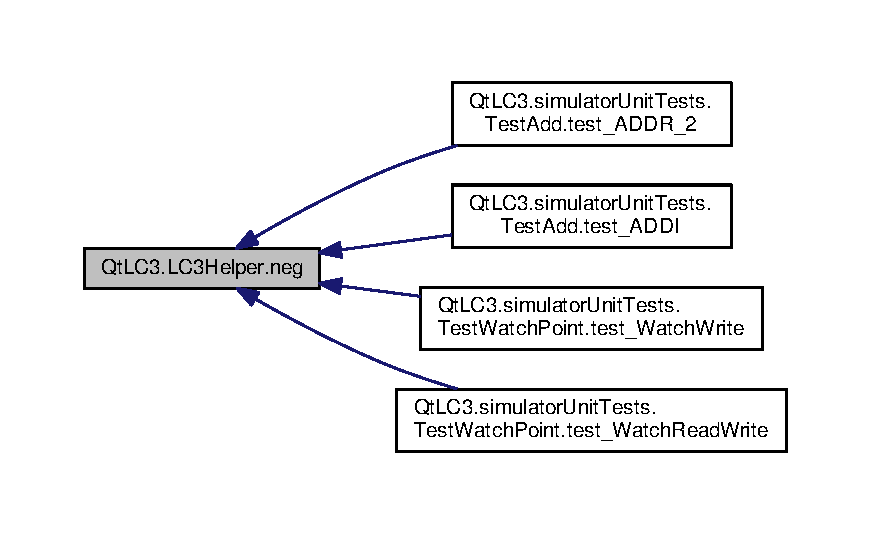
\includegraphics[width=350pt]{namespace_qt_l_c3_1_1_l_c3_helper_a66561d57b2b0ccc464240f7983019ef7_icgraph}
\end{center}
\end{figure}


\hypertarget{namespace_qt_l_c3_1_1_l_c3_helper_a922cbc23ef2e88f72e3ffb8823b3448e}{\index{Qt\-L\-C3\-::\-L\-C3\-Helper@{Qt\-L\-C3\-::\-L\-C3\-Helper}!S\-E\-T\-B\-A\-S\-E\-R@{S\-E\-T\-B\-A\-S\-E\-R}}
\index{S\-E\-T\-B\-A\-S\-E\-R@{S\-E\-T\-B\-A\-S\-E\-R}!QtLC3::LC3Helper@{Qt\-L\-C3\-::\-L\-C3\-Helper}}
\subsubsection[{S\-E\-T\-B\-A\-S\-E\-R}]{\setlength{\rightskip}{0pt plus 5cm}def Qt\-L\-C3.\-L\-C3\-Helper.\-S\-E\-T\-B\-A\-S\-E\-R (
\begin{DoxyParamCaption}
\item[{}]{x}
\end{DoxyParamCaption}
)}}\label{namespace_qt_l_c3_1_1_l_c3_helper_a922cbc23ef2e88f72e3ffb8823b3448e}


Definition at line 5 of file L\-C3\-Helper.\-py.

\hypertarget{namespace_qt_l_c3_1_1_l_c3_helper_ae7cb9e4899acd35e8916ea0b1f2cfd72}{\index{Qt\-L\-C3\-::\-L\-C3\-Helper@{Qt\-L\-C3\-::\-L\-C3\-Helper}!S\-E\-T\-D\-R@{S\-E\-T\-D\-R}}
\index{S\-E\-T\-D\-R@{S\-E\-T\-D\-R}!QtLC3::LC3Helper@{Qt\-L\-C3\-::\-L\-C3\-Helper}}
\subsubsection[{S\-E\-T\-D\-R}]{\setlength{\rightskip}{0pt plus 5cm}def Qt\-L\-C3.\-L\-C3\-Helper.\-S\-E\-T\-D\-R (
\begin{DoxyParamCaption}
\item[{}]{x}
\end{DoxyParamCaption}
)}}\label{namespace_qt_l_c3_1_1_l_c3_helper_ae7cb9e4899acd35e8916ea0b1f2cfd72}


Definition at line 1 of file L\-C3\-Helper.\-py.

\hypertarget{namespace_qt_l_c3_1_1_l_c3_helper_aa3a2d3ee10a9fb5f5638cc4a8c2636f5}{\index{Qt\-L\-C3\-::\-L\-C3\-Helper@{Qt\-L\-C3\-::\-L\-C3\-Helper}!S\-E\-T\-N@{S\-E\-T\-N}}
\index{S\-E\-T\-N@{S\-E\-T\-N}!QtLC3::LC3Helper@{Qt\-L\-C3\-::\-L\-C3\-Helper}}
\subsubsection[{S\-E\-T\-N}]{\setlength{\rightskip}{0pt plus 5cm}def Qt\-L\-C3.\-L\-C3\-Helper.\-S\-E\-T\-N (
\begin{DoxyParamCaption}
\item[{}]{x}
\end{DoxyParamCaption}
)}}\label{namespace_qt_l_c3_1_1_l_c3_helper_aa3a2d3ee10a9fb5f5638cc4a8c2636f5}


Definition at line 9 of file L\-C3\-Helper.\-py.

\hypertarget{namespace_qt_l_c3_1_1_l_c3_helper_a185a0d60d8df4193d5eef92513b34b65}{\index{Qt\-L\-C3\-::\-L\-C3\-Helper@{Qt\-L\-C3\-::\-L\-C3\-Helper}!S\-E\-T\-P@{S\-E\-T\-P}}
\index{S\-E\-T\-P@{S\-E\-T\-P}!QtLC3::LC3Helper@{Qt\-L\-C3\-::\-L\-C3\-Helper}}
\subsubsection[{S\-E\-T\-P}]{\setlength{\rightskip}{0pt plus 5cm}def Qt\-L\-C3.\-L\-C3\-Helper.\-S\-E\-T\-P (
\begin{DoxyParamCaption}
\item[{}]{x}
\end{DoxyParamCaption}
)}}\label{namespace_qt_l_c3_1_1_l_c3_helper_a185a0d60d8df4193d5eef92513b34b65}


Definition at line 13 of file L\-C3\-Helper.\-py.

\hypertarget{namespace_qt_l_c3_1_1_l_c3_helper_a3864324a32466dcc102bc13bbd16bb68}{\index{Qt\-L\-C3\-::\-L\-C3\-Helper@{Qt\-L\-C3\-::\-L\-C3\-Helper}!S\-E\-T\-S\-R1@{S\-E\-T\-S\-R1}}
\index{S\-E\-T\-S\-R1@{S\-E\-T\-S\-R1}!QtLC3::LC3Helper@{Qt\-L\-C3\-::\-L\-C3\-Helper}}
\subsubsection[{S\-E\-T\-S\-R1}]{\setlength{\rightskip}{0pt plus 5cm}def Qt\-L\-C3.\-L\-C3\-Helper.\-S\-E\-T\-S\-R1 (
\begin{DoxyParamCaption}
\item[{}]{x}
\end{DoxyParamCaption}
)}}\label{namespace_qt_l_c3_1_1_l_c3_helper_a3864324a32466dcc102bc13bbd16bb68}


Definition at line 3 of file L\-C3\-Helper.\-py.

\hypertarget{namespace_qt_l_c3_1_1_l_c3_helper_a89ace97b16bf0b0cf2f2d5ccc0a7d041}{\index{Qt\-L\-C3\-::\-L\-C3\-Helper@{Qt\-L\-C3\-::\-L\-C3\-Helper}!S\-E\-T\-S\-R2@{S\-E\-T\-S\-R2}}
\index{S\-E\-T\-S\-R2@{S\-E\-T\-S\-R2}!QtLC3::LC3Helper@{Qt\-L\-C3\-::\-L\-C3\-Helper}}
\subsubsection[{S\-E\-T\-S\-R2}]{\setlength{\rightskip}{0pt plus 5cm}def Qt\-L\-C3.\-L\-C3\-Helper.\-S\-E\-T\-S\-R2 (
\begin{DoxyParamCaption}
\item[{}]{x}
\end{DoxyParamCaption}
)}}\label{namespace_qt_l_c3_1_1_l_c3_helper_a89ace97b16bf0b0cf2f2d5ccc0a7d041}


Definition at line 7 of file L\-C3\-Helper.\-py.

\hypertarget{namespace_qt_l_c3_1_1_l_c3_helper_a1046fcb8930de46a28d181523a37ed12}{\index{Qt\-L\-C3\-::\-L\-C3\-Helper@{Qt\-L\-C3\-::\-L\-C3\-Helper}!S\-E\-T\-Z@{S\-E\-T\-Z}}
\index{S\-E\-T\-Z@{S\-E\-T\-Z}!QtLC3::LC3Helper@{Qt\-L\-C3\-::\-L\-C3\-Helper}}
\subsubsection[{S\-E\-T\-Z}]{\setlength{\rightskip}{0pt plus 5cm}def Qt\-L\-C3.\-L\-C3\-Helper.\-S\-E\-T\-Z (
\begin{DoxyParamCaption}
\item[{}]{x}
\end{DoxyParamCaption}
)}}\label{namespace_qt_l_c3_1_1_l_c3_helper_a1046fcb8930de46a28d181523a37ed12}


Definition at line 11 of file L\-C3\-Helper.\-py.



\subsection{Variable Documentation}
\hypertarget{namespace_qt_l_c3_1_1_l_c3_helper_a870d6aff07b57f130171b8de8762429f}{\index{Qt\-L\-C3\-::\-L\-C3\-Helper@{Qt\-L\-C3\-::\-L\-C3\-Helper}!A\-D\-D\-I@{A\-D\-D\-I}}
\index{A\-D\-D\-I@{A\-D\-D\-I}!QtLC3::LC3Helper@{Qt\-L\-C3\-::\-L\-C3\-Helper}}
\subsubsection[{A\-D\-D\-I}]{\setlength{\rightskip}{0pt plus 5cm}Qt\-L\-C3.\-L\-C3\-Helper.\-A\-D\-D\-I = {\bf A\-D\-D\-R}$\vert${\bf S\-T\-E\-E\-R\-I\-N\-G\-N\-O\-R\-M}}}\label{namespace_qt_l_c3_1_1_l_c3_helper_a870d6aff07b57f130171b8de8762429f}


Definition at line 20 of file L\-C3\-Helper.\-py.

\hypertarget{namespace_qt_l_c3_1_1_l_c3_helper_a2755d6265d2b3b158525ab68e253bc53}{\index{Qt\-L\-C3\-::\-L\-C3\-Helper@{Qt\-L\-C3\-::\-L\-C3\-Helper}!A\-D\-D\-R@{A\-D\-D\-R}}
\index{A\-D\-D\-R@{A\-D\-D\-R}!QtLC3::LC3Helper@{Qt\-L\-C3\-::\-L\-C3\-Helper}}
\subsubsection[{A\-D\-D\-R}]{\setlength{\rightskip}{0pt plus 5cm}int Qt\-L\-C3.\-L\-C3\-Helper.\-A\-D\-D\-R = 0x1000}}\label{namespace_qt_l_c3_1_1_l_c3_helper_a2755d6265d2b3b158525ab68e253bc53}


Definition at line 19 of file L\-C3\-Helper.\-py.

\hypertarget{namespace_qt_l_c3_1_1_l_c3_helper_a74183f176a3d37fb085953d31270977b}{\index{Qt\-L\-C3\-::\-L\-C3\-Helper@{Qt\-L\-C3\-::\-L\-C3\-Helper}!A\-N\-D\-I@{A\-N\-D\-I}}
\index{A\-N\-D\-I@{A\-N\-D\-I}!QtLC3::LC3Helper@{Qt\-L\-C3\-::\-L\-C3\-Helper}}
\subsubsection[{A\-N\-D\-I}]{\setlength{\rightskip}{0pt plus 5cm}Qt\-L\-C3.\-L\-C3\-Helper.\-A\-N\-D\-I = {\bf A\-N\-D\-R}$\vert${\bf S\-T\-E\-E\-R\-I\-N\-G\-N\-O\-R\-M}}}\label{namespace_qt_l_c3_1_1_l_c3_helper_a74183f176a3d37fb085953d31270977b}


Definition at line 22 of file L\-C3\-Helper.\-py.

\hypertarget{namespace_qt_l_c3_1_1_l_c3_helper_a708c0a74889a4ebe74b3b4aca5a689f0}{\index{Qt\-L\-C3\-::\-L\-C3\-Helper@{Qt\-L\-C3\-::\-L\-C3\-Helper}!A\-N\-D\-R@{A\-N\-D\-R}}
\index{A\-N\-D\-R@{A\-N\-D\-R}!QtLC3::LC3Helper@{Qt\-L\-C3\-::\-L\-C3\-Helper}}
\subsubsection[{A\-N\-D\-R}]{\setlength{\rightskip}{0pt plus 5cm}int Qt\-L\-C3.\-L\-C3\-Helper.\-A\-N\-D\-R = 0x5000}}\label{namespace_qt_l_c3_1_1_l_c3_helper_a708c0a74889a4ebe74b3b4aca5a689f0}


Definition at line 21 of file L\-C3\-Helper.\-py.

\hypertarget{namespace_qt_l_c3_1_1_l_c3_helper_a149ab214faca1440f8e8af5aaabbf655}{\index{Qt\-L\-C3\-::\-L\-C3\-Helper@{Qt\-L\-C3\-::\-L\-C3\-Helper}!B\-R@{B\-R}}
\index{B\-R@{B\-R}!QtLC3::LC3Helper@{Qt\-L\-C3\-::\-L\-C3\-Helper}}
\subsubsection[{B\-R}]{\setlength{\rightskip}{0pt plus 5cm}int Qt\-L\-C3.\-L\-C3\-Helper.\-B\-R = 0x0000}}\label{namespace_qt_l_c3_1_1_l_c3_helper_a149ab214faca1440f8e8af5aaabbf655}


Definition at line 23 of file L\-C3\-Helper.\-py.

\hypertarget{namespace_qt_l_c3_1_1_l_c3_helper_a9cfcb139adf16a156aa0e870bfc85a7d}{\index{Qt\-L\-C3\-::\-L\-C3\-Helper@{Qt\-L\-C3\-::\-L\-C3\-Helper}!J\-M\-P@{J\-M\-P}}
\index{J\-M\-P@{J\-M\-P}!QtLC3::LC3Helper@{Qt\-L\-C3\-::\-L\-C3\-Helper}}
\subsubsection[{J\-M\-P}]{\setlength{\rightskip}{0pt plus 5cm}int Qt\-L\-C3.\-L\-C3\-Helper.\-J\-M\-P = 0x\-C000}}\label{namespace_qt_l_c3_1_1_l_c3_helper_a9cfcb139adf16a156aa0e870bfc85a7d}


Definition at line 24 of file L\-C3\-Helper.\-py.

\hypertarget{namespace_qt_l_c3_1_1_l_c3_helper_a152d613276c3ea907e432835077675e4}{\index{Qt\-L\-C3\-::\-L\-C3\-Helper@{Qt\-L\-C3\-::\-L\-C3\-Helper}!J\-S\-R@{J\-S\-R}}
\index{J\-S\-R@{J\-S\-R}!QtLC3::LC3Helper@{Qt\-L\-C3\-::\-L\-C3\-Helper}}
\subsubsection[{J\-S\-R}]{\setlength{\rightskip}{0pt plus 5cm}int Qt\-L\-C3.\-L\-C3\-Helper.\-J\-S\-R = 0x4800}}\label{namespace_qt_l_c3_1_1_l_c3_helper_a152d613276c3ea907e432835077675e4}


Definition at line 25 of file L\-C3\-Helper.\-py.

\hypertarget{namespace_qt_l_c3_1_1_l_c3_helper_abf6d27ff681f7adc316c548fd3c3ef01}{\index{Qt\-L\-C3\-::\-L\-C3\-Helper@{Qt\-L\-C3\-::\-L\-C3\-Helper}!J\-S\-R\-R@{J\-S\-R\-R}}
\index{J\-S\-R\-R@{J\-S\-R\-R}!QtLC3::LC3Helper@{Qt\-L\-C3\-::\-L\-C3\-Helper}}
\subsubsection[{J\-S\-R\-R}]{\setlength{\rightskip}{0pt plus 5cm}int Qt\-L\-C3.\-L\-C3\-Helper.\-J\-S\-R\-R = 0x4000}}\label{namespace_qt_l_c3_1_1_l_c3_helper_abf6d27ff681f7adc316c548fd3c3ef01}


Definition at line 26 of file L\-C3\-Helper.\-py.

\hypertarget{namespace_qt_l_c3_1_1_l_c3_helper_a967020a01ae6b98a4730fe11bf09b508}{\index{Qt\-L\-C3\-::\-L\-C3\-Helper@{Qt\-L\-C3\-::\-L\-C3\-Helper}!L\-D@{L\-D}}
\index{L\-D@{L\-D}!QtLC3::LC3Helper@{Qt\-L\-C3\-::\-L\-C3\-Helper}}
\subsubsection[{L\-D}]{\setlength{\rightskip}{0pt plus 5cm}int Qt\-L\-C3.\-L\-C3\-Helper.\-L\-D = 0x2000}}\label{namespace_qt_l_c3_1_1_l_c3_helper_a967020a01ae6b98a4730fe11bf09b508}


Definition at line 27 of file L\-C3\-Helper.\-py.

\hypertarget{namespace_qt_l_c3_1_1_l_c3_helper_a102fef9d0708f7b9d1f6af3a541ed5fa}{\index{Qt\-L\-C3\-::\-L\-C3\-Helper@{Qt\-L\-C3\-::\-L\-C3\-Helper}!L\-D\-I@{L\-D\-I}}
\index{L\-D\-I@{L\-D\-I}!QtLC3::LC3Helper@{Qt\-L\-C3\-::\-L\-C3\-Helper}}
\subsubsection[{L\-D\-I}]{\setlength{\rightskip}{0pt plus 5cm}int Qt\-L\-C3.\-L\-C3\-Helper.\-L\-D\-I = 0x\-A000}}\label{namespace_qt_l_c3_1_1_l_c3_helper_a102fef9d0708f7b9d1f6af3a541ed5fa}


Definition at line 28 of file L\-C3\-Helper.\-py.

\hypertarget{namespace_qt_l_c3_1_1_l_c3_helper_a671ecbeb3d540e5d11929c18d3ff37f7}{\index{Qt\-L\-C3\-::\-L\-C3\-Helper@{Qt\-L\-C3\-::\-L\-C3\-Helper}!L\-D\-R@{L\-D\-R}}
\index{L\-D\-R@{L\-D\-R}!QtLC3::LC3Helper@{Qt\-L\-C3\-::\-L\-C3\-Helper}}
\subsubsection[{L\-D\-R}]{\setlength{\rightskip}{0pt plus 5cm}int Qt\-L\-C3.\-L\-C3\-Helper.\-L\-D\-R = 0x6000}}\label{namespace_qt_l_c3_1_1_l_c3_helper_a671ecbeb3d540e5d11929c18d3ff37f7}


Definition at line 29 of file L\-C3\-Helper.\-py.

\hypertarget{namespace_qt_l_c3_1_1_l_c3_helper_a6582e54ef243974ac33d19bdef271a30}{\index{Qt\-L\-C3\-::\-L\-C3\-Helper@{Qt\-L\-C3\-::\-L\-C3\-Helper}!L\-E\-A@{L\-E\-A}}
\index{L\-E\-A@{L\-E\-A}!QtLC3::LC3Helper@{Qt\-L\-C3\-::\-L\-C3\-Helper}}
\subsubsection[{L\-E\-A}]{\setlength{\rightskip}{0pt plus 5cm}int Qt\-L\-C3.\-L\-C3\-Helper.\-L\-E\-A = 0x\-E000}}\label{namespace_qt_l_c3_1_1_l_c3_helper_a6582e54ef243974ac33d19bdef271a30}


Definition at line 30 of file L\-C3\-Helper.\-py.

\hypertarget{namespace_qt_l_c3_1_1_l_c3_helper_a801523098ae57c18b172eac2319261fd}{\index{Qt\-L\-C3\-::\-L\-C3\-Helper@{Qt\-L\-C3\-::\-L\-C3\-Helper}!N\-O\-T@{N\-O\-T}}
\index{N\-O\-T@{N\-O\-T}!QtLC3::LC3Helper@{Qt\-L\-C3\-::\-L\-C3\-Helper}}
\subsubsection[{N\-O\-T}]{\setlength{\rightskip}{0pt plus 5cm}int Qt\-L\-C3.\-L\-C3\-Helper.\-N\-O\-T = 0x903\-F}}\label{namespace_qt_l_c3_1_1_l_c3_helper_a801523098ae57c18b172eac2319261fd}


Definition at line 31 of file L\-C3\-Helper.\-py.

\hypertarget{namespace_qt_l_c3_1_1_l_c3_helper_aefa011a0063f0a58973debd03508c067}{\index{Qt\-L\-C3\-::\-L\-C3\-Helper@{Qt\-L\-C3\-::\-L\-C3\-Helper}!R\-E\-T@{R\-E\-T}}
\index{R\-E\-T@{R\-E\-T}!QtLC3::LC3Helper@{Qt\-L\-C3\-::\-L\-C3\-Helper}}
\subsubsection[{R\-E\-T}]{\setlength{\rightskip}{0pt plus 5cm}int Qt\-L\-C3.\-L\-C3\-Helper.\-R\-E\-T = 0x\-C000}}\label{namespace_qt_l_c3_1_1_l_c3_helper_aefa011a0063f0a58973debd03508c067}


Definition at line 32 of file L\-C3\-Helper.\-py.

\hypertarget{namespace_qt_l_c3_1_1_l_c3_helper_a39240b80276cf60d71330cb051c7f5f8}{\index{Qt\-L\-C3\-::\-L\-C3\-Helper@{Qt\-L\-C3\-::\-L\-C3\-Helper}!R\-T\-I@{R\-T\-I}}
\index{R\-T\-I@{R\-T\-I}!QtLC3::LC3Helper@{Qt\-L\-C3\-::\-L\-C3\-Helper}}
\subsubsection[{R\-T\-I}]{\setlength{\rightskip}{0pt plus 5cm}int Qt\-L\-C3.\-L\-C3\-Helper.\-R\-T\-I = 0x8000}}\label{namespace_qt_l_c3_1_1_l_c3_helper_a39240b80276cf60d71330cb051c7f5f8}


Definition at line 33 of file L\-C3\-Helper.\-py.

\hypertarget{namespace_qt_l_c3_1_1_l_c3_helper_ae050a048ad522e75de8c065c20f01bb8}{\index{Qt\-L\-C3\-::\-L\-C3\-Helper@{Qt\-L\-C3\-::\-L\-C3\-Helper}!S\-T@{S\-T}}
\index{S\-T@{S\-T}!QtLC3::LC3Helper@{Qt\-L\-C3\-::\-L\-C3\-Helper}}
\subsubsection[{S\-T}]{\setlength{\rightskip}{0pt plus 5cm}int Qt\-L\-C3.\-L\-C3\-Helper.\-S\-T = 0x3000}}\label{namespace_qt_l_c3_1_1_l_c3_helper_ae050a048ad522e75de8c065c20f01bb8}


Definition at line 34 of file L\-C3\-Helper.\-py.

\hypertarget{namespace_qt_l_c3_1_1_l_c3_helper_ac1252434698120b0fe5f93491268215f}{\index{Qt\-L\-C3\-::\-L\-C3\-Helper@{Qt\-L\-C3\-::\-L\-C3\-Helper}!S\-T\-E\-E\-R\-I\-N\-G\-N\-O\-R\-M@{S\-T\-E\-E\-R\-I\-N\-G\-N\-O\-R\-M}}
\index{S\-T\-E\-E\-R\-I\-N\-G\-N\-O\-R\-M@{S\-T\-E\-E\-R\-I\-N\-G\-N\-O\-R\-M}!QtLC3::LC3Helper@{Qt\-L\-C3\-::\-L\-C3\-Helper}}
\subsubsection[{S\-T\-E\-E\-R\-I\-N\-G\-N\-O\-R\-M}]{\setlength{\rightskip}{0pt plus 5cm}int Qt\-L\-C3.\-L\-C3\-Helper.\-S\-T\-E\-E\-R\-I\-N\-G\-N\-O\-R\-M = 1}}\label{namespace_qt_l_c3_1_1_l_c3_helper_ac1252434698120b0fe5f93491268215f}


Definition at line 18 of file L\-C3\-Helper.\-py.

\hypertarget{namespace_qt_l_c3_1_1_l_c3_helper_a98e7ada71d9f15520c276fa797e1343f}{\index{Qt\-L\-C3\-::\-L\-C3\-Helper@{Qt\-L\-C3\-::\-L\-C3\-Helper}!S\-T\-I@{S\-T\-I}}
\index{S\-T\-I@{S\-T\-I}!QtLC3::LC3Helper@{Qt\-L\-C3\-::\-L\-C3\-Helper}}
\subsubsection[{S\-T\-I}]{\setlength{\rightskip}{0pt plus 5cm}int Qt\-L\-C3.\-L\-C3\-Helper.\-S\-T\-I = 0x\-B000}}\label{namespace_qt_l_c3_1_1_l_c3_helper_a98e7ada71d9f15520c276fa797e1343f}


Definition at line 35 of file L\-C3\-Helper.\-py.

\hypertarget{namespace_qt_l_c3_1_1_l_c3_helper_a64d7a91288d9d2de515dd63e71c0c25a}{\index{Qt\-L\-C3\-::\-L\-C3\-Helper@{Qt\-L\-C3\-::\-L\-C3\-Helper}!S\-T\-R@{S\-T\-R}}
\index{S\-T\-R@{S\-T\-R}!QtLC3::LC3Helper@{Qt\-L\-C3\-::\-L\-C3\-Helper}}
\subsubsection[{S\-T\-R}]{\setlength{\rightskip}{0pt plus 5cm}int Qt\-L\-C3.\-L\-C3\-Helper.\-S\-T\-R = 0x7000}}\label{namespace_qt_l_c3_1_1_l_c3_helper_a64d7a91288d9d2de515dd63e71c0c25a}


Definition at line 36 of file L\-C3\-Helper.\-py.

\hypertarget{namespace_qt_l_c3_1_1_l_c3_helper_ad70fb630058318d34edec66d1e3e4b6e}{\index{Qt\-L\-C3\-::\-L\-C3\-Helper@{Qt\-L\-C3\-::\-L\-C3\-Helper}!T\-R\-A\-P@{T\-R\-A\-P}}
\index{T\-R\-A\-P@{T\-R\-A\-P}!QtLC3::LC3Helper@{Qt\-L\-C3\-::\-L\-C3\-Helper}}
\subsubsection[{T\-R\-A\-P}]{\setlength{\rightskip}{0pt plus 5cm}int Qt\-L\-C3.\-L\-C3\-Helper.\-T\-R\-A\-P = 0x\-F000}}\label{namespace_qt_l_c3_1_1_l_c3_helper_ad70fb630058318d34edec66d1e3e4b6e}


Definition at line 37 of file L\-C3\-Helper.\-py.


\hypertarget{namespace_qt_l_c3_1_1pylc3sim}{\section{Qt\-L\-C3.\-pylc3sim Namespace Reference}
\label{namespace_qt_l_c3_1_1pylc3sim}\index{Qt\-L\-C3.\-pylc3sim@{Qt\-L\-C3.\-pylc3sim}}
}
\subsection*{Classes}
\begin{DoxyCompactItemize}
\item 
class \hyperlink{class_qt_l_c3_1_1pylc3sim_1_1py_l_c3_sim}{py\-L\-C3\-Sim}
\end{DoxyCompactItemize}

\hypertarget{namespace_qt_l_c3_1_1simulator_unit_tests}{\section{Qt\-L\-C3.\-simulator\-Unit\-Tests Namespace Reference}
\label{namespace_qt_l_c3_1_1simulator_unit_tests}\index{Qt\-L\-C3.\-simulator\-Unit\-Tests@{Qt\-L\-C3.\-simulator\-Unit\-Tests}}
}
\subsection*{Classes}
\begin{DoxyCompactItemize}
\item 
class \hyperlink{class_qt_l_c3_1_1simulator_unit_tests_1_1_test_add}{Test\-Add}
\item 
class \hyperlink{class_qt_l_c3_1_1simulator_unit_tests_1_1_test_and}{Test\-And}
\item 
class \hyperlink{class_qt_l_c3_1_1simulator_unit_tests_1_1_test_watch_point}{Test\-Watch\-Point}
\end{DoxyCompactItemize}
\subsection*{Functions}
\begin{DoxyCompactItemize}
\item 
def \hyperlink{namespace_qt_l_c3_1_1simulator_unit_tests_a2d038a14c4230b686d46e0e427e8941e}{do\-Test}
\end{DoxyCompactItemize}
\subsection*{Variables}
\begin{DoxyCompactItemize}
\item 
\hyperlink{namespace_qt_l_c3_1_1simulator_unit_tests_a762ffb74f9f8e380299cd1c525932310}{false} = False
\item 
\hyperlink{namespace_qt_l_c3_1_1simulator_unit_tests_ac23f444832b767cf808b54d5d6f4bd72}{true} = True
\end{DoxyCompactItemize}


\subsection{Function Documentation}
\hypertarget{namespace_qt_l_c3_1_1simulator_unit_tests_a2d038a14c4230b686d46e0e427e8941e}{\index{Qt\-L\-C3\-::simulator\-Unit\-Tests@{Qt\-L\-C3\-::simulator\-Unit\-Tests}!do\-Test@{do\-Test}}
\index{do\-Test@{do\-Test}!QtLC3::simulatorUnitTests@{Qt\-L\-C3\-::simulator\-Unit\-Tests}}
\subsubsection[{do\-Test}]{\setlength{\rightskip}{0pt plus 5cm}def Qt\-L\-C3.\-simulator\-Unit\-Tests.\-do\-Test (
\begin{DoxyParamCaption}
\item[{}]{test\-Case}
\end{DoxyParamCaption}
)}}\label{namespace_qt_l_c3_1_1simulator_unit_tests_a2d038a14c4230b686d46e0e427e8941e}


Definition at line 147 of file simulator\-Unit\-Tests.\-py.



\subsection{Variable Documentation}
\hypertarget{namespace_qt_l_c3_1_1simulator_unit_tests_a762ffb74f9f8e380299cd1c525932310}{\index{Qt\-L\-C3\-::simulator\-Unit\-Tests@{Qt\-L\-C3\-::simulator\-Unit\-Tests}!false@{false}}
\index{false@{false}!QtLC3::simulatorUnitTests@{Qt\-L\-C3\-::simulator\-Unit\-Tests}}
\subsubsection[{false}]{\setlength{\rightskip}{0pt plus 5cm}Qt\-L\-C3.\-simulator\-Unit\-Tests.\-false = False}}\label{namespace_qt_l_c3_1_1simulator_unit_tests_a762ffb74f9f8e380299cd1c525932310}


Definition at line 6 of file simulator\-Unit\-Tests.\-py.

\hypertarget{namespace_qt_l_c3_1_1simulator_unit_tests_ac23f444832b767cf808b54d5d6f4bd72}{\index{Qt\-L\-C3\-::simulator\-Unit\-Tests@{Qt\-L\-C3\-::simulator\-Unit\-Tests}!true@{true}}
\index{true@{true}!QtLC3::simulatorUnitTests@{Qt\-L\-C3\-::simulator\-Unit\-Tests}}
\subsubsection[{true}]{\setlength{\rightskip}{0pt plus 5cm}Qt\-L\-C3.\-simulator\-Unit\-Tests.\-true = True}}\label{namespace_qt_l_c3_1_1simulator_unit_tests_ac23f444832b767cf808b54d5d6f4bd72}


Definition at line 7 of file simulator\-Unit\-Tests.\-py.


\hypertarget{namespace_qt_l_c3_1_1sorting_test}{\section{Qt\-L\-C3.\-sorting\-Test Namespace Reference}
\label{namespace_qt_l_c3_1_1sorting_test}\index{Qt\-L\-C3.\-sorting\-Test@{Qt\-L\-C3.\-sorting\-Test}}
}
\subsection*{Classes}
\begin{DoxyCompactItemize}
\item 
class \hyperlink{class_qt_l_c3_1_1sorting_test_1_1_sorting_test}{Sorting\-Test}
\end{DoxyCompactItemize}
\subsection*{Functions}
\begin{DoxyCompactItemize}
\item 
def \hyperlink{namespace_qt_l_c3_1_1sorting_test_a60151bfd7e175f8f0c56327890bf6de2}{upper\-Half}
\item 
def \hyperlink{namespace_qt_l_c3_1_1sorting_test_a05c0d265a8257814f488eb5baf0b6fb1}{lower\-Half}
\end{DoxyCompactItemize}


\subsection{Function Documentation}
\hypertarget{namespace_qt_l_c3_1_1sorting_test_a05c0d265a8257814f488eb5baf0b6fb1}{\index{Qt\-L\-C3\-::sorting\-Test@{Qt\-L\-C3\-::sorting\-Test}!lower\-Half@{lower\-Half}}
\index{lower\-Half@{lower\-Half}!QtLC3::sortingTest@{Qt\-L\-C3\-::sorting\-Test}}
\subsubsection[{lower\-Half}]{\setlength{\rightskip}{0pt plus 5cm}def Qt\-L\-C3.\-sorting\-Test.\-lower\-Half (
\begin{DoxyParamCaption}
\item[{}]{x}
\end{DoxyParamCaption}
)}}\label{namespace_qt_l_c3_1_1sorting_test_a05c0d265a8257814f488eb5baf0b6fb1}


Definition at line 24 of file sorting\-Test.\-py.



Here is the caller graph for this function\-:
\nopagebreak
\begin{figure}[H]
\begin{center}
\leavevmode
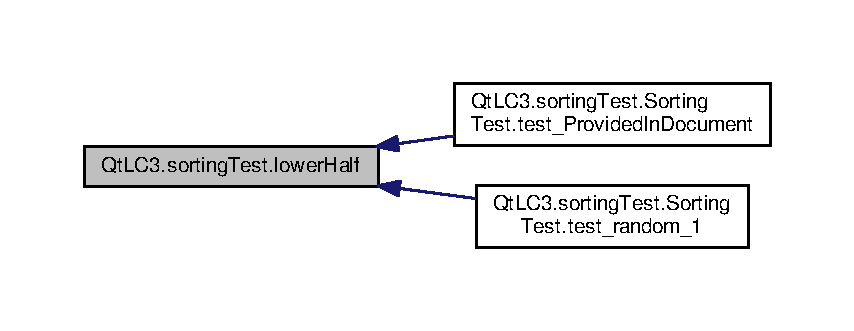
\includegraphics[width=350pt]{namespace_qt_l_c3_1_1sorting_test_a05c0d265a8257814f488eb5baf0b6fb1_icgraph}
\end{center}
\end{figure}


\hypertarget{namespace_qt_l_c3_1_1sorting_test_a60151bfd7e175f8f0c56327890bf6de2}{\index{Qt\-L\-C3\-::sorting\-Test@{Qt\-L\-C3\-::sorting\-Test}!upper\-Half@{upper\-Half}}
\index{upper\-Half@{upper\-Half}!QtLC3::sortingTest@{Qt\-L\-C3\-::sorting\-Test}}
\subsubsection[{upper\-Half}]{\setlength{\rightskip}{0pt plus 5cm}def Qt\-L\-C3.\-sorting\-Test.\-upper\-Half (
\begin{DoxyParamCaption}
\item[{}]{x}
\end{DoxyParamCaption}
)}}\label{namespace_qt_l_c3_1_1sorting_test_a60151bfd7e175f8f0c56327890bf6de2}


Definition at line 21 of file sorting\-Test.\-py.



Here is the caller graph for this function\-:
\nopagebreak
\begin{figure}[H]
\begin{center}
\leavevmode
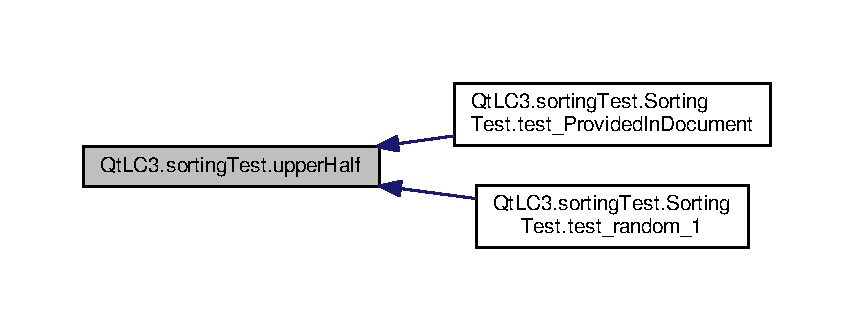
\includegraphics[width=350pt]{namespace_qt_l_c3_1_1sorting_test_a60151bfd7e175f8f0c56327890bf6de2_icgraph}
\end{center}
\end{figure}



\hypertarget{namespacesorting_test}{\section{sorting\-Test Namespace Reference}
\label{namespacesorting_test}\index{sorting\-Test@{sorting\-Test}}
}
\subsection*{Classes}
\begin{DoxyCompactItemize}
\item 
class \hyperlink{classsorting_test_1_1_sorting_test}{Sorting\-Test}
\end{DoxyCompactItemize}
\subsection*{Functions}
\begin{DoxyCompactItemize}
\item 
def \hyperlink{namespacesorting_test_a053e72abcbfaaa5a0a3ce799a4e820f7}{upper\-Half}
\item 
def \hyperlink{namespacesorting_test_a6c56b012d5be2f3958634adfabd4ee6e}{lower\-Half}
\end{DoxyCompactItemize}


\subsection{Function Documentation}
\hypertarget{namespacesorting_test_a6c56b012d5be2f3958634adfabd4ee6e}{\index{sorting\-Test@{sorting\-Test}!lower\-Half@{lower\-Half}}
\index{lower\-Half@{lower\-Half}!sortingTest@{sorting\-Test}}
\subsubsection[{lower\-Half}]{\setlength{\rightskip}{0pt plus 5cm}def sorting\-Test.\-lower\-Half (
\begin{DoxyParamCaption}
\item[{}]{x}
\end{DoxyParamCaption}
)}}\label{namespacesorting_test_a6c56b012d5be2f3958634adfabd4ee6e}


Definition at line 23 of file sorting\-Test.\-py.



Here is the caller graph for this function\-:
\nopagebreak
\begin{figure}[H]
\begin{center}
\leavevmode
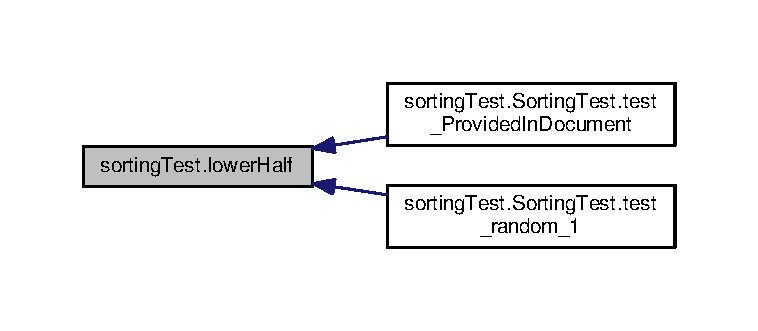
\includegraphics[width=350pt]{namespacesorting_test_a6c56b012d5be2f3958634adfabd4ee6e_icgraph}
\end{center}
\end{figure}


\hypertarget{namespacesorting_test_a053e72abcbfaaa5a0a3ce799a4e820f7}{\index{sorting\-Test@{sorting\-Test}!upper\-Half@{upper\-Half}}
\index{upper\-Half@{upper\-Half}!sortingTest@{sorting\-Test}}
\subsubsection[{upper\-Half}]{\setlength{\rightskip}{0pt plus 5cm}def sorting\-Test.\-upper\-Half (
\begin{DoxyParamCaption}
\item[{}]{x}
\end{DoxyParamCaption}
)}}\label{namespacesorting_test_a053e72abcbfaaa5a0a3ce799a4e820f7}


Definition at line 20 of file sorting\-Test.\-py.



Here is the caller graph for this function\-:
\nopagebreak
\begin{figure}[H]
\begin{center}
\leavevmode
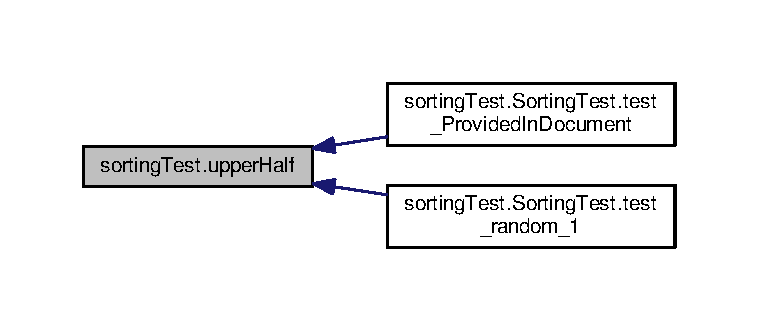
\includegraphics[width=350pt]{namespacesorting_test_a053e72abcbfaaa5a0a3ce799a4e820f7_icgraph}
\end{center}
\end{figure}



\chapter{Class Documentation}
\hypertarget{class_lc3_sim}{\section{Lc3\-Sim Class Reference}
\label{class_lc3_sim}\index{Lc3\-Sim@{Lc3\-Sim}}
}


{\ttfamily \#include $<$lc3sim.\-h$>$}

\subsection*{Public Member Functions}
\begin{DoxyCompactItemize}
\item 
\hyperlink{class_lc3_sim_acc78232c60f0708da3a04f702695fa38}{Lc3\-Sim} ()
\end{DoxyCompactItemize}


\subsection{Detailed Description}


Definition at line 4 of file lc3sim.\-h.



\subsection{Constructor \& Destructor Documentation}
\hypertarget{class_lc3_sim_acc78232c60f0708da3a04f702695fa38}{\index{Lc3\-Sim@{Lc3\-Sim}!Lc3\-Sim@{Lc3\-Sim}}
\index{Lc3\-Sim@{Lc3\-Sim}!Lc3Sim@{Lc3\-Sim}}
\subsubsection[{Lc3\-Sim}]{\setlength{\rightskip}{0pt plus 5cm}Lc3\-Sim\-::\-Lc3\-Sim (
\begin{DoxyParamCaption}
{}
\end{DoxyParamCaption}
)}}\label{class_lc3_sim_acc78232c60f0708da3a04f702695fa38}


The documentation for this class was generated from the following file\-:\begin{DoxyCompactItemize}
\item 
\hyperlink{lc3sim_8h}{lc3sim.\-h}\end{DoxyCompactItemize}

\hypertarget{class_qt_l_c3_1_1pylc3sim_1_1py_l_c3_sim}{\section{Qt\-L\-C3.\-pylc3sim.\-py\-L\-C3\-Sim Class Reference}
\label{class_qt_l_c3_1_1pylc3sim_1_1py_l_c3_sim}\index{Qt\-L\-C3.\-pylc3sim.\-py\-L\-C3\-Sim@{Qt\-L\-C3.\-pylc3sim.\-py\-L\-C3\-Sim}}
}


Inheritance diagram for Qt\-L\-C3.\-pylc3sim.\-py\-L\-C3\-Sim\-:
\nopagebreak
\begin{figure}[H]
\begin{center}
\leavevmode
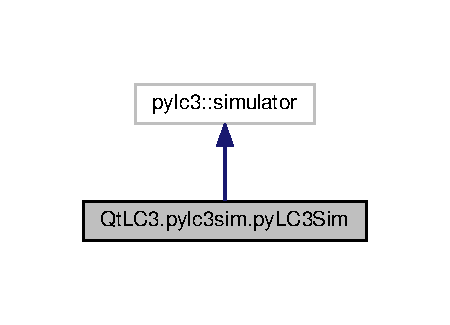
\includegraphics[width=216pt]{class_qt_l_c3_1_1pylc3sim_1_1py_l_c3_sim__inherit__graph}
\end{center}
\end{figure}


Collaboration diagram for Qt\-L\-C3.\-pylc3sim.\-py\-L\-C3\-Sim\-:
\nopagebreak
\begin{figure}[H]
\begin{center}
\leavevmode
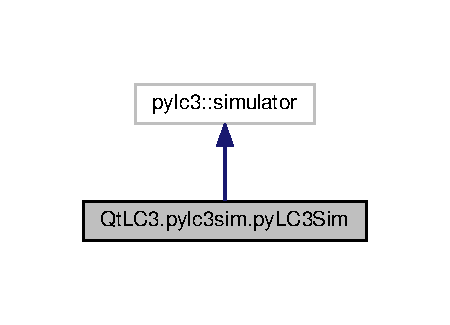
\includegraphics[width=216pt]{class_qt_l_c3_1_1pylc3sim_1_1py_l_c3_sim__coll__graph}
\end{center}
\end{figure}
\subsection*{Public Member Functions}
\begin{DoxyCompactItemize}
\item 
def \hyperlink{class_qt_l_c3_1_1pylc3sim_1_1py_l_c3_sim_a25625c1944d9a66775f712e7b35dcca3}{\-\_\-\-\_\-init\-\_\-\-\_\-}
\end{DoxyCompactItemize}
\subsection*{Public Attributes}
\begin{DoxyCompactItemize}
\item 
\hyperlink{class_qt_l_c3_1_1pylc3sim_1_1py_l_c3_sim_a4c69adaa23258cb7fbf052069f69daf5}{mem}
\end{DoxyCompactItemize}


\subsection{Detailed Description}


Definition at line 5 of file pylc3sim.\-py.



\subsection{Constructor \& Destructor Documentation}
\hypertarget{class_qt_l_c3_1_1pylc3sim_1_1py_l_c3_sim_a25625c1944d9a66775f712e7b35dcca3}{\index{Qt\-L\-C3\-::pylc3sim\-::py\-L\-C3\-Sim@{Qt\-L\-C3\-::pylc3sim\-::py\-L\-C3\-Sim}!\-\_\-\-\_\-init\-\_\-\-\_\-@{\-\_\-\-\_\-init\-\_\-\-\_\-}}
\index{\-\_\-\-\_\-init\-\_\-\-\_\-@{\-\_\-\-\_\-init\-\_\-\-\_\-}!QtLC3::pylc3sim::pyLC3Sim@{Qt\-L\-C3\-::pylc3sim\-::py\-L\-C3\-Sim}}
\subsubsection[{\-\_\-\-\_\-init\-\_\-\-\_\-}]{\setlength{\rightskip}{0pt plus 5cm}def Qt\-L\-C3.\-pylc3sim.\-py\-L\-C3\-Sim.\-\_\-\-\_\-init\-\_\-\-\_\- (
\begin{DoxyParamCaption}
\item[{}]{self}
\end{DoxyParamCaption}
)}}\label{class_qt_l_c3_1_1pylc3sim_1_1py_l_c3_sim_a25625c1944d9a66775f712e7b35dcca3}


Definition at line 7 of file pylc3sim.\-py.



\subsection{Member Data Documentation}
\hypertarget{class_qt_l_c3_1_1pylc3sim_1_1py_l_c3_sim_a4c69adaa23258cb7fbf052069f69daf5}{\index{Qt\-L\-C3\-::pylc3sim\-::py\-L\-C3\-Sim@{Qt\-L\-C3\-::pylc3sim\-::py\-L\-C3\-Sim}!mem@{mem}}
\index{mem@{mem}!QtLC3::pylc3sim::pyLC3Sim@{Qt\-L\-C3\-::pylc3sim\-::py\-L\-C3\-Sim}}
\subsubsection[{mem}]{\setlength{\rightskip}{0pt plus 5cm}Qt\-L\-C3.\-pylc3sim.\-py\-L\-C3\-Sim.\-mem}}\label{class_qt_l_c3_1_1pylc3sim_1_1py_l_c3_sim_a4c69adaa23258cb7fbf052069f69daf5}


Definition at line 11 of file pylc3sim.\-py.



The documentation for this class was generated from the following file\-:\begin{DoxyCompactItemize}
\item 
\hyperlink{pylc3sim_8py}{pylc3sim.\-py}\end{DoxyCompactItemize}

\hypertarget{classsimulator}{\section{simulator Class Reference}
\label{classsimulator}\index{simulator@{simulator}}
}


Basic L\-C3 Simulator Class.  




{\ttfamily \#include $<$simulator.\-hpp$>$}



Collaboration diagram for simulator\-:
\nopagebreak
\begin{figure}[H]
\begin{center}
\leavevmode
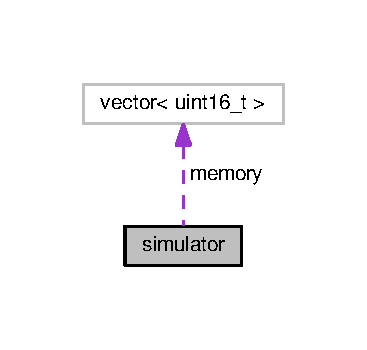
\includegraphics[width=176pt]{classsimulator__coll__graph}
\end{center}
\end{figure}
\subsection*{Public Types}
\begin{DoxyCompactItemize}
\item 
using \hyperlink{classsimulator_af29328ef8d8d6120a91a379c2801b44b}{M\-E\-M\-\_\-type} = vector$<$ uint16\-\_\-t $>$
\end{DoxyCompactItemize}
\subsection*{Public Member Functions}
\begin{DoxyCompactItemize}
\item 
bool \hyperlink{classsimulator_a0b627c7dfa086c2e712447f6f52df45a}{step\-N} (int cycles)
\begin{DoxyCompactList}\small\item\em step forward N cycles \end{DoxyCompactList}\item 
bool \hyperlink{classsimulator_a22bf3281b0165d3d93fb71658b19fdb8}{do\-Inst} (uint16\-\_\-t)
\begin{DoxyCompactList}\small\item\em Process an instruction. \end{DoxyCompactList}\item 
vector$<$ uint16\-\_\-t $>$ \hyperlink{classsimulator_a67f2ca29746d88a463751c5eba137f8c}{slice\-Mem} (uint16\-\_\-t start, uint16\-\_\-t stop)
\begin{DoxyCompactList}\small\item\em Get a slice of memory. \end{DoxyCompactList}\item 
uint16\-\_\-t \hyperlink{classsimulator_adf34711d9ba2ef3e98dea9600a44576d}{get\-Reg} (int number)
\begin{DoxyCompactList}\small\item\em Read from the register file. \end{DoxyCompactList}\item 
bool \hyperlink{classsimulator_a99ff28d7459e1e5634f78aa204e1b81b}{set\-Reg} (int number, uint16\-\_\-t new\-Val)
\begin{DoxyCompactList}\small\item\em Write to the register file. \end{DoxyCompactList}\item 
bool \hyperlink{classsimulator_a9cc84c8d70c5095de7ea0e3cf6ff3164}{get\-Pcsr\-Bit} (char mnemonic)
\begin{DoxyCompactList}\small\item\em Get a status bit from the P\-S\-R. \end{DoxyCompactList}\item 
bool \hyperlink{classsimulator_a6cc07560fc476a4d733b8c5ff6925351}{set\-Pcsr\-Bit} (char mnemonic, bool new\-Val)
\begin{DoxyCompactList}\small\item\em Set status bit in P\-S\-R. \end{DoxyCompactList}\item 
uint16\-\_\-t \hyperlink{classsimulator_ada54a778a08fd580bf17ba2599f0bca6}{get\-P\-C} (void)
\begin{DoxyCompactList}\small\item\em Set the Current P\-C. \end{DoxyCompactList}\item 
bool \hyperlink{classsimulator_a20809a32770f874231c60dec97215728}{set\-P\-C} (uint16\-\_\-t)
\item 
bool \hyperlink{classsimulator_aac9ba2b60a6fcbd7ec0da971e0b7c93b}{add\-Watch\-Point} (uint16\-\_\-t addr, bool read, bool write, Py\-Object $\ast$cb)
\begin{DoxyCompactList}\small\item\em Add a watch point to the simulator. \end{DoxyCompactList}\item 
int \hyperlink{classsimulator_a2eaf15124121f4df2711370063436d76}{get\-Num\-Watch\-Points} ()
\begin{DoxyCompactList}\small\item\em Helper function returns number of watch points. \end{DoxyCompactList}\item 
bool \hyperlink{classsimulator_a6df3804bda4d00dab0859b1b143974c9}{load\-Bin\-File} (std\-::string)
\begin{DoxyCompactList}\small\item\em Load a L\-C3 Object file. \end{DoxyCompactList}\end{DoxyCompactItemize}
\subsection*{Public Attributes}
\begin{DoxyCompactItemize}
\item 
vector$<$ uint16\-\_\-t $>$ \hyperlink{classsimulator_a7c49313a87678b1737725b6bf695119d}{memory} = vector$<$uint16\-\_\-t$>$(\hyperlink{simulator_8hpp_aeacd5eb3350ee895e5e2f56398f1055c}{A\-D\-D\-R\-E\-S\-S\-\_\-\-S\-P\-A\-C\-E})
\end{DoxyCompactItemize}


\subsection{Detailed Description}
Basic L\-C3 Simulator Class. 

This class is exposed to the Python Interface, C\-L\-I, and G\-U\-I 

Definition at line 33 of file simulator.\-hpp.



\subsection{Member Typedef Documentation}
\hypertarget{classsimulator_af29328ef8d8d6120a91a379c2801b44b}{\index{simulator@{simulator}!M\-E\-M\-\_\-type@{M\-E\-M\-\_\-type}}
\index{M\-E\-M\-\_\-type@{M\-E\-M\-\_\-type}!simulator@{simulator}}
\subsubsection[{M\-E\-M\-\_\-type}]{\setlength{\rightskip}{0pt plus 5cm}using {\bf simulator\-::\-M\-E\-M\-\_\-type} =  vector$<$uint16\-\_\-t$>$}}\label{classsimulator_af29328ef8d8d6120a91a379c2801b44b}


Definition at line 35 of file simulator.\-hpp.



\subsection{Member Function Documentation}
\hypertarget{classsimulator_aac9ba2b60a6fcbd7ec0da971e0b7c93b}{\index{simulator@{simulator}!add\-Watch\-Point@{add\-Watch\-Point}}
\index{add\-Watch\-Point@{add\-Watch\-Point}!simulator@{simulator}}
\subsubsection[{add\-Watch\-Point}]{\setlength{\rightskip}{0pt plus 5cm}bool simulator\-::add\-Watch\-Point (
\begin{DoxyParamCaption}
\item[{uint16\-\_\-t}]{addr, }
\item[{bool}]{read, }
\item[{bool}]{write, }
\item[{Py\-Object $\ast$}]{cb}
\end{DoxyParamCaption}
)}}\label{classsimulator_aac9ba2b60a6fcbd7ec0da971e0b7c93b}


Add a watch point to the simulator. 

Watch points can be triggered on any combination of read/write to a specific address. On triggering, the watchpoints call a python callback function to handle the event. These call backs could be as simple as a print statement. It also accepts python lambdas.


\begin{DoxyParams}{Parameters}
{\em addr} & Address of memory to watch \\
\hline
{\em read} & trigger on mem read \\
\hline
{\em write} & trigger on mem write \\
\hline
{\em cb} & call back function on event triggered \\
\hline
\end{DoxyParams}
\begin{DoxyReturn}{Returns}
successful? 
\end{DoxyReturn}


Definition at line 369 of file simulator.\-cpp.



Here is the caller graph for this function\-:
\nopagebreak
\begin{figure}[H]
\begin{center}
\leavevmode
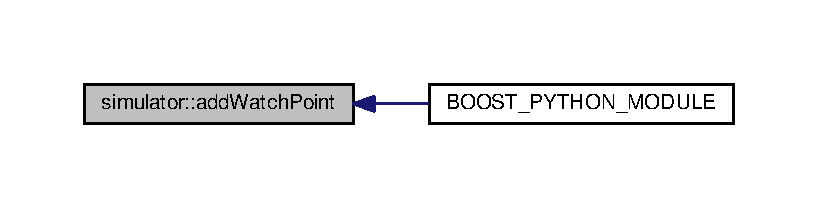
\includegraphics[width=350pt]{classsimulator_aac9ba2b60a6fcbd7ec0da971e0b7c93b_icgraph}
\end{center}
\end{figure}


\hypertarget{classsimulator_a22bf3281b0165d3d93fb71658b19fdb8}{\index{simulator@{simulator}!do\-Inst@{do\-Inst}}
\index{do\-Inst@{do\-Inst}!simulator@{simulator}}
\subsubsection[{do\-Inst}]{\setlength{\rightskip}{0pt plus 5cm}bool simulator\-::do\-Inst (
\begin{DoxyParamCaption}
\item[{uint16\-\_\-t}]{inst}
\end{DoxyParamCaption}
)}}\label{classsimulator_a22bf3281b0165d3d93fb71658b19fdb8}


Process an instruction. 

This is equivelent to decode execute


\begin{DoxyParams}{Parameters}
{\em inst} & 16 bit instruction to process \\
\hline
\end{DoxyParams}
\begin{DoxyReturn}{Returns}
exception occurred? 
\end{DoxyReturn}


Definition at line 133 of file simulator.\-cpp.



Here is the caller graph for this function\-:
\nopagebreak
\begin{figure}[H]
\begin{center}
\leavevmode
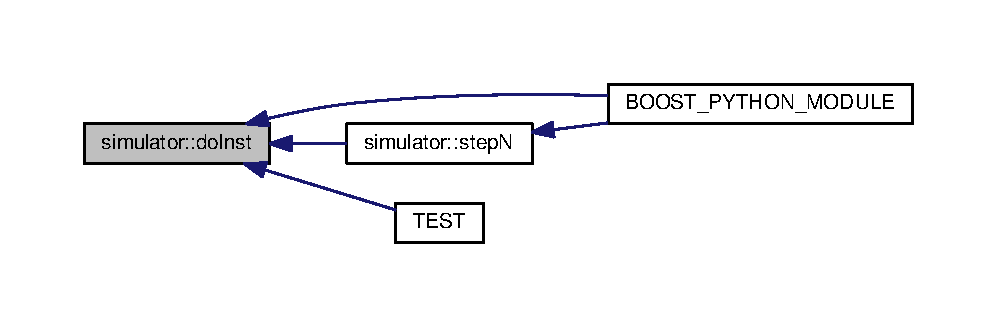
\includegraphics[width=350pt]{classsimulator_a22bf3281b0165d3d93fb71658b19fdb8_icgraph}
\end{center}
\end{figure}


\hypertarget{classsimulator_a2eaf15124121f4df2711370063436d76}{\index{simulator@{simulator}!get\-Num\-Watch\-Points@{get\-Num\-Watch\-Points}}
\index{get\-Num\-Watch\-Points@{get\-Num\-Watch\-Points}!simulator@{simulator}}
\subsubsection[{get\-Num\-Watch\-Points}]{\setlength{\rightskip}{0pt plus 5cm}int simulator\-::get\-Num\-Watch\-Points (
\begin{DoxyParamCaption}
{}
\end{DoxyParamCaption}
)}}\label{classsimulator_a2eaf15124121f4df2711370063436d76}


Helper function returns number of watch points. 

\begin{DoxyReturn}{Returns}
number of watchpoints 
\end{DoxyReturn}


Definition at line 386 of file simulator.\-cpp.



Here is the caller graph for this function\-:
\nopagebreak
\begin{figure}[H]
\begin{center}
\leavevmode
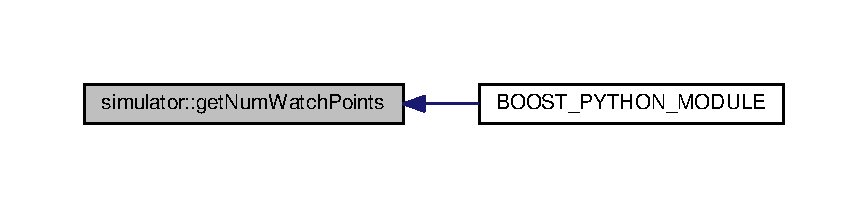
\includegraphics[width=350pt]{classsimulator_a2eaf15124121f4df2711370063436d76_icgraph}
\end{center}
\end{figure}


\hypertarget{classsimulator_ada54a778a08fd580bf17ba2599f0bca6}{\index{simulator@{simulator}!get\-P\-C@{get\-P\-C}}
\index{get\-P\-C@{get\-P\-C}!simulator@{simulator}}
\subsubsection[{get\-P\-C}]{\setlength{\rightskip}{0pt plus 5cm}uint16\-\_\-t simulator\-::get\-P\-C (
\begin{DoxyParamCaption}
\item[{void}]{}
\end{DoxyParamCaption}
)}}\label{classsimulator_ada54a778a08fd580bf17ba2599f0bca6}


Set the Current P\-C. 

Checks if the desired P\-C is Valid, then sets it \begin{DoxyReturn}{Returns}
boolean if valid or not 
\end{DoxyReturn}


Definition at line 349 of file simulator.\-cpp.



Here is the caller graph for this function\-:
\nopagebreak
\begin{figure}[H]
\begin{center}
\leavevmode
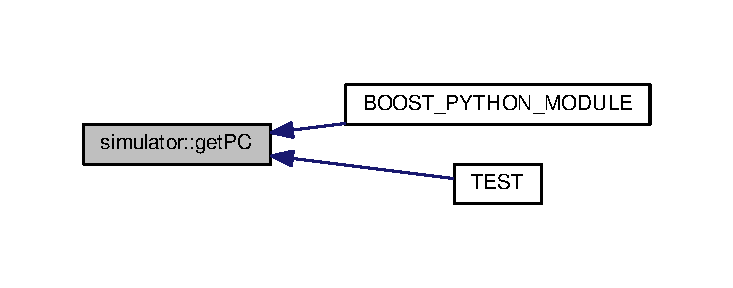
\includegraphics[width=350pt]{classsimulator_ada54a778a08fd580bf17ba2599f0bca6_icgraph}
\end{center}
\end{figure}


\hypertarget{classsimulator_a9cc84c8d70c5095de7ea0e3cf6ff3164}{\index{simulator@{simulator}!get\-Pcsr\-Bit@{get\-Pcsr\-Bit}}
\index{get\-Pcsr\-Bit@{get\-Pcsr\-Bit}!simulator@{simulator}}
\subsubsection[{get\-Pcsr\-Bit}]{\setlength{\rightskip}{0pt plus 5cm}bool simulator\-::get\-Pcsr\-Bit (
\begin{DoxyParamCaption}
\item[{char}]{mnemonic}
\end{DoxyParamCaption}
)}}\label{classsimulator_a9cc84c8d70c5095de7ea0e3cf6ff3164}


Get a status bit from the P\-S\-R. 

request a status bit from the P\-S\-R using its character


\begin{DoxyParams}{Parameters}
{\em mnemonic} & n, z, p, or s \\
\hline
\end{DoxyParams}
\begin{DoxyReturn}{Returns}
the status bit 
\end{DoxyReturn}


Definition at line 250 of file simulator.\-cpp.



Here is the caller graph for this function\-:
\nopagebreak
\begin{figure}[H]
\begin{center}
\leavevmode
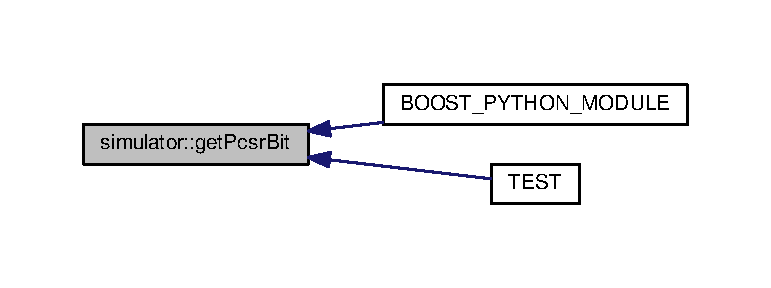
\includegraphics[width=350pt]{classsimulator_a9cc84c8d70c5095de7ea0e3cf6ff3164_icgraph}
\end{center}
\end{figure}


\hypertarget{classsimulator_adf34711d9ba2ef3e98dea9600a44576d}{\index{simulator@{simulator}!get\-Reg@{get\-Reg}}
\index{get\-Reg@{get\-Reg}!simulator@{simulator}}
\subsubsection[{get\-Reg}]{\setlength{\rightskip}{0pt plus 5cm}uint16\-\_\-t simulator\-::get\-Reg (
\begin{DoxyParamCaption}
\item[{int}]{number}
\end{DoxyParamCaption}
)}}\label{classsimulator_adf34711d9ba2ef3e98dea9600a44576d}


Read from the register file. 

Read from the register file


\begin{DoxyParams}{Parameters}
{\em number} & Register Number \\
\hline
\end{DoxyParams}
\begin{DoxyReturn}{Returns}
register data 
\end{DoxyReturn}


Definition at line 308 of file simulator.\-cpp.



Here is the caller graph for this function\-:
\nopagebreak
\begin{figure}[H]
\begin{center}
\leavevmode
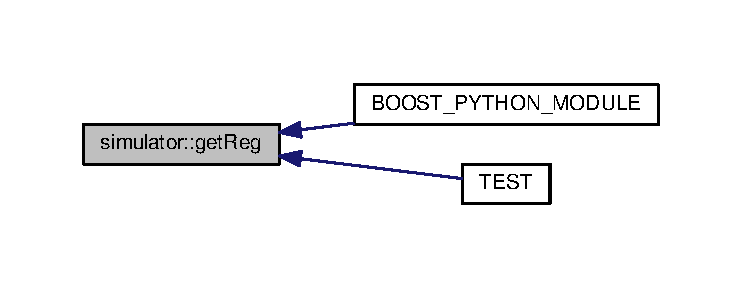
\includegraphics[width=350pt]{classsimulator_adf34711d9ba2ef3e98dea9600a44576d_icgraph}
\end{center}
\end{figure}


\hypertarget{classsimulator_a6df3804bda4d00dab0859b1b143974c9}{\index{simulator@{simulator}!load\-Bin\-File@{load\-Bin\-File}}
\index{load\-Bin\-File@{load\-Bin\-File}!simulator@{simulator}}
\subsubsection[{load\-Bin\-File}]{\setlength{\rightskip}{0pt plus 5cm}bool simulator\-::load\-Bin\-File (
\begin{DoxyParamCaption}
\item[{std\-::string}]{filename}
\end{DoxyParamCaption}
)}}\label{classsimulator_a6df3804bda4d00dab0859b1b143974c9}


Load a L\-C3 Object file. 

L\-C3 object files are binary files where the first word denotes the starting address of the program


\begin{DoxyParams}{Parameters}
{\em filename} & path to file \\
\hline
\end{DoxyParams}
\begin{DoxyReturn}{Returns}
successful? 
\end{DoxyReturn}


Definition at line 31 of file simulator.\-cpp.



Here is the caller graph for this function\-:
\nopagebreak
\begin{figure}[H]
\begin{center}
\leavevmode
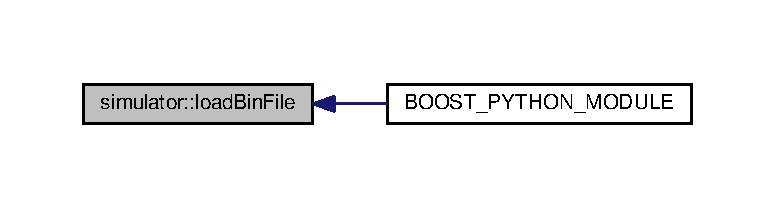
\includegraphics[width=350pt]{classsimulator_a6df3804bda4d00dab0859b1b143974c9_icgraph}
\end{center}
\end{figure}


\hypertarget{classsimulator_a20809a32770f874231c60dec97215728}{\index{simulator@{simulator}!set\-P\-C@{set\-P\-C}}
\index{set\-P\-C@{set\-P\-C}!simulator@{simulator}}
\subsubsection[{set\-P\-C}]{\setlength{\rightskip}{0pt plus 5cm}bool simulator\-::set\-P\-C (
\begin{DoxyParamCaption}
\item[{uint16\-\_\-t}]{pc}
\end{DoxyParamCaption}
)}}\label{classsimulator_a20809a32770f874231c60dec97215728}


Definition at line 350 of file simulator.\-cpp.



Here is the caller graph for this function\-:
\nopagebreak
\begin{figure}[H]
\begin{center}
\leavevmode
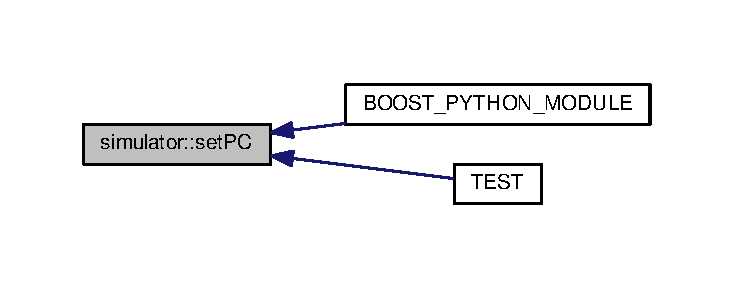
\includegraphics[width=350pt]{classsimulator_a20809a32770f874231c60dec97215728_icgraph}
\end{center}
\end{figure}


\hypertarget{classsimulator_a6cc07560fc476a4d733b8c5ff6925351}{\index{simulator@{simulator}!set\-Pcsr\-Bit@{set\-Pcsr\-Bit}}
\index{set\-Pcsr\-Bit@{set\-Pcsr\-Bit}!simulator@{simulator}}
\subsubsection[{set\-Pcsr\-Bit}]{\setlength{\rightskip}{0pt plus 5cm}bool simulator\-::set\-Pcsr\-Bit (
\begin{DoxyParamCaption}
\item[{char}]{mnemonic, }
\item[{bool}]{new\-Val}
\end{DoxyParamCaption}
)}}\label{classsimulator_a6cc07560fc476a4d733b8c5ff6925351}


Set status bit in P\-S\-R. 

Set a specific status bit in the P\-S\-R


\begin{DoxyParams}{Parameters}
{\em mnemonic} & character of bit to set \\
\hline
{\em new\-Val} & true/false\\
\hline
\end{DoxyParams}
\begin{DoxyReturn}{Returns}
successful? 
\end{DoxyReturn}


Definition at line 279 of file simulator.\-cpp.



Here is the caller graph for this function\-:
\nopagebreak
\begin{figure}[H]
\begin{center}
\leavevmode
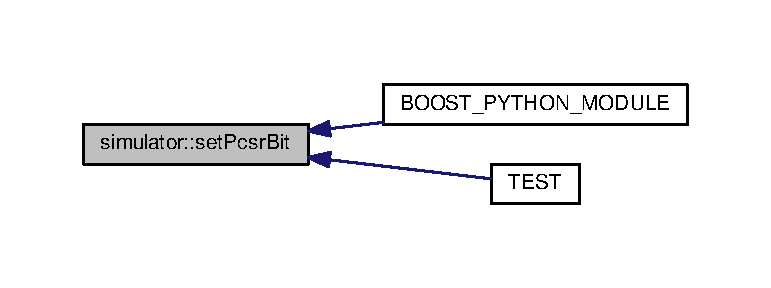
\includegraphics[width=350pt]{classsimulator_a6cc07560fc476a4d733b8c5ff6925351_icgraph}
\end{center}
\end{figure}


\hypertarget{classsimulator_a99ff28d7459e1e5634f78aa204e1b81b}{\index{simulator@{simulator}!set\-Reg@{set\-Reg}}
\index{set\-Reg@{set\-Reg}!simulator@{simulator}}
\subsubsection[{set\-Reg}]{\setlength{\rightskip}{0pt plus 5cm}bool simulator\-::set\-Reg (
\begin{DoxyParamCaption}
\item[{int}]{number, }
\item[{uint16\-\_\-t}]{new\-Val}
\end{DoxyParamCaption}
)}}\label{classsimulator_a99ff28d7459e1e5634f78aa204e1b81b}


Write to the register file. 

Write to the register file


\begin{DoxyParams}{Parameters}
{\em number} & Register Number \\
\hline
{\em new\-Val} & reg $<$= new\-Val\\
\hline
\end{DoxyParams}
\begin{DoxyReturn}{Returns}
successful? 
\end{DoxyReturn}


Definition at line 321 of file simulator.\-cpp.



Here is the caller graph for this function\-:
\nopagebreak
\begin{figure}[H]
\begin{center}
\leavevmode
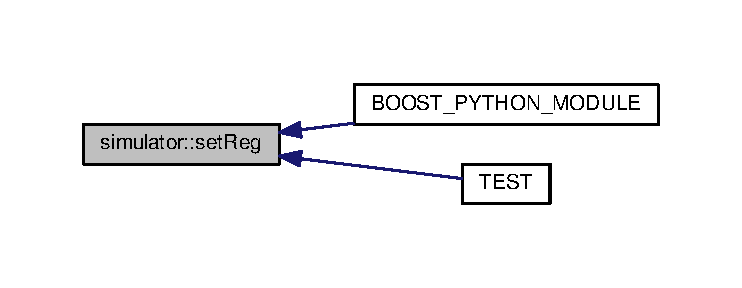
\includegraphics[width=350pt]{classsimulator_a99ff28d7459e1e5634f78aa204e1b81b_icgraph}
\end{center}
\end{figure}


\hypertarget{classsimulator_a67f2ca29746d88a463751c5eba137f8c}{\index{simulator@{simulator}!slice\-Mem@{slice\-Mem}}
\index{slice\-Mem@{slice\-Mem}!simulator@{simulator}}
\subsubsection[{slice\-Mem}]{\setlength{\rightskip}{0pt plus 5cm}vector$<$ uint16\-\_\-t $>$ simulator\-::slice\-Mem (
\begin{DoxyParamCaption}
\item[{uint16\-\_\-t}]{start, }
\item[{uint16\-\_\-t}]{stop}
\end{DoxyParamCaption}
)}}\label{classsimulator_a67f2ca29746d88a463751c5eba137f8c}


Get a slice of memory. 

get a slice of memory to work with


\begin{DoxyParams}{Parameters}
{\em start} & starting address \\
\hline
{\em stop} & end address\\
\hline
\end{DoxyParams}
\begin{DoxyReturn}{Returns}
a copy of a slice of memory 
\end{DoxyReturn}


Definition at line 339 of file simulator.\-cpp.

\hypertarget{classsimulator_a0b627c7dfa086c2e712447f6f52df45a}{\index{simulator@{simulator}!step\-N@{step\-N}}
\index{step\-N@{step\-N}!simulator@{simulator}}
\subsubsection[{step\-N}]{\setlength{\rightskip}{0pt plus 5cm}bool simulator\-::step\-N (
\begin{DoxyParamCaption}
\item[{int}]{cycles}
\end{DoxyParamCaption}
)}}\label{classsimulator_a0b627c7dfa086c2e712447f6f52df45a}


step forward N cycles 

step forward N cycles


\begin{DoxyParams}{Parameters}
{\em cycles} & number of cycles to step \\
\hline
\end{DoxyParams}
\begin{DoxyReturn}{Returns}
false if exception occurred 
\end{DoxyReturn}


Definition at line 13 of file simulator.\-cpp.



Here is the call graph for this function\-:
\nopagebreak
\begin{figure}[H]
\begin{center}
\leavevmode
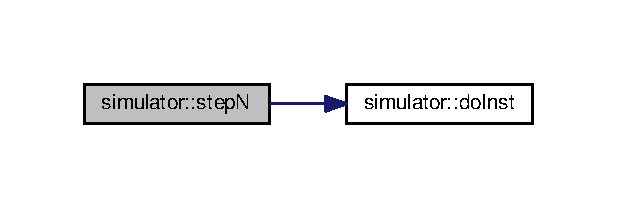
\includegraphics[width=296pt]{classsimulator_a0b627c7dfa086c2e712447f6f52df45a_cgraph}
\end{center}
\end{figure}




Here is the caller graph for this function\-:
\nopagebreak
\begin{figure}[H]
\begin{center}
\leavevmode
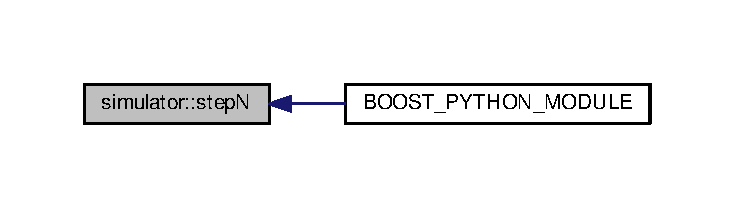
\includegraphics[width=350pt]{classsimulator_a0b627c7dfa086c2e712447f6f52df45a_icgraph}
\end{center}
\end{figure}




\subsection{Member Data Documentation}
\hypertarget{classsimulator_a7c49313a87678b1737725b6bf695119d}{\index{simulator@{simulator}!memory@{memory}}
\index{memory@{memory}!simulator@{simulator}}
\subsubsection[{memory}]{\setlength{\rightskip}{0pt plus 5cm}vector$<$uint16\-\_\-t$>$ simulator\-::memory = vector$<$uint16\-\_\-t$>$({\bf A\-D\-D\-R\-E\-S\-S\-\_\-\-S\-P\-A\-C\-E})}}\label{classsimulator_a7c49313a87678b1737725b6bf695119d}


Definition at line 36 of file simulator.\-hpp.



The documentation for this class was generated from the following files\-:\begin{DoxyCompactItemize}
\item 
\hyperlink{simulator_8hpp}{simulator.\-hpp}\item 
\hyperlink{simulator_8cpp}{simulator.\-cpp}\end{DoxyCompactItemize}

\hypertarget{class_qt_l_c3_1_1sorting_test_1_1_sorting_test}{\section{Qt\-L\-C3.\-sorting\-Test.\-Sorting\-Test Class Reference}
\label{class_qt_l_c3_1_1sorting_test_1_1_sorting_test}\index{Qt\-L\-C3.\-sorting\-Test.\-Sorting\-Test@{Qt\-L\-C3.\-sorting\-Test.\-Sorting\-Test}}
}


Inheritance diagram for Qt\-L\-C3.\-sorting\-Test.\-Sorting\-Test\-:
\nopagebreak
\begin{figure}[H]
\begin{center}
\leavevmode
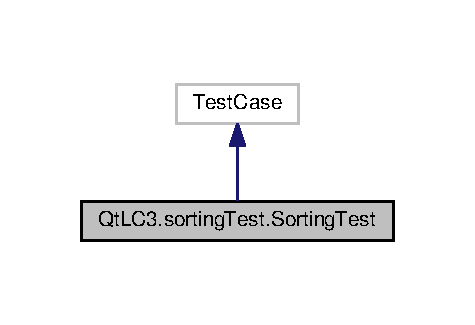
\includegraphics[width=228pt]{class_qt_l_c3_1_1sorting_test_1_1_sorting_test__inherit__graph}
\end{center}
\end{figure}


Collaboration diagram for Qt\-L\-C3.\-sorting\-Test.\-Sorting\-Test\-:
\nopagebreak
\begin{figure}[H]
\begin{center}
\leavevmode
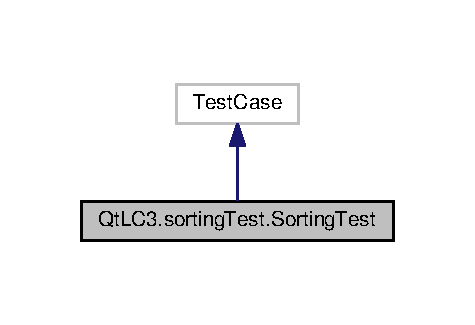
\includegraphics[width=228pt]{class_qt_l_c3_1_1sorting_test_1_1_sorting_test__coll__graph}
\end{center}
\end{figure}
\subsection*{Public Member Functions}
\begin{DoxyCompactItemize}
\item 
def \hyperlink{class_qt_l_c3_1_1sorting_test_1_1_sorting_test_ad72a050cb8e3fc0a3d27ae6a614d1fa2}{set\-Up}
\item 
def \hyperlink{class_qt_l_c3_1_1sorting_test_1_1_sorting_test_a8fbda524442059a1390ad64031af6a97}{test\-\_\-\-Provided\-In\-Document}
\item 
def \hyperlink{class_qt_l_c3_1_1sorting_test_1_1_sorting_test_a98bd681eacb66a9ed2f7ca3389c88d0c}{test\-\_\-random\-\_\-1}
\end{DoxyCompactItemize}
\subsection*{Public Attributes}
\begin{DoxyCompactItemize}
\item 
\hyperlink{class_qt_l_c3_1_1sorting_test_1_1_sorting_test_a7c42c3f120e66c3a19d29aa0e4afc9ec}{sim}
\end{DoxyCompactItemize}


\subsection{Detailed Description}


Definition at line 27 of file sorting\-Test.\-py.



\subsection{Member Function Documentation}
\hypertarget{class_qt_l_c3_1_1sorting_test_1_1_sorting_test_ad72a050cb8e3fc0a3d27ae6a614d1fa2}{\index{Qt\-L\-C3\-::sorting\-Test\-::\-Sorting\-Test@{Qt\-L\-C3\-::sorting\-Test\-::\-Sorting\-Test}!set\-Up@{set\-Up}}
\index{set\-Up@{set\-Up}!QtLC3::sortingTest::SortingTest@{Qt\-L\-C3\-::sorting\-Test\-::\-Sorting\-Test}}
\subsubsection[{set\-Up}]{\setlength{\rightskip}{0pt plus 5cm}def Qt\-L\-C3.\-sorting\-Test.\-Sorting\-Test.\-set\-Up (
\begin{DoxyParamCaption}
\item[{}]{self}
\end{DoxyParamCaption}
)}}\label{class_qt_l_c3_1_1sorting_test_1_1_sorting_test_ad72a050cb8e3fc0a3d27ae6a614d1fa2}


Definition at line 30 of file sorting\-Test.\-py.

\hypertarget{class_qt_l_c3_1_1sorting_test_1_1_sorting_test_a8fbda524442059a1390ad64031af6a97}{\index{Qt\-L\-C3\-::sorting\-Test\-::\-Sorting\-Test@{Qt\-L\-C3\-::sorting\-Test\-::\-Sorting\-Test}!test\-\_\-\-Provided\-In\-Document@{test\-\_\-\-Provided\-In\-Document}}
\index{test\-\_\-\-Provided\-In\-Document@{test\-\_\-\-Provided\-In\-Document}!QtLC3::sortingTest::SortingTest@{Qt\-L\-C3\-::sorting\-Test\-::\-Sorting\-Test}}
\subsubsection[{test\-\_\-\-Provided\-In\-Document}]{\setlength{\rightskip}{0pt plus 5cm}def Qt\-L\-C3.\-sorting\-Test.\-Sorting\-Test.\-test\-\_\-\-Provided\-In\-Document (
\begin{DoxyParamCaption}
\item[{}]{self}
\end{DoxyParamCaption}
)}}\label{class_qt_l_c3_1_1sorting_test_1_1_sorting_test_a8fbda524442059a1390ad64031af6a97}


Definition at line 35 of file sorting\-Test.\-py.



Here is the call graph for this function\-:
\nopagebreak
\begin{figure}[H]
\begin{center}
\leavevmode
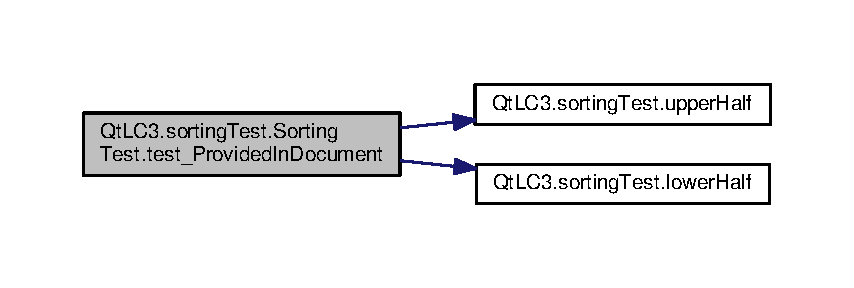
\includegraphics[width=350pt]{class_qt_l_c3_1_1sorting_test_1_1_sorting_test_a8fbda524442059a1390ad64031af6a97_cgraph}
\end{center}
\end{figure}


\hypertarget{class_qt_l_c3_1_1sorting_test_1_1_sorting_test_a98bd681eacb66a9ed2f7ca3389c88d0c}{\index{Qt\-L\-C3\-::sorting\-Test\-::\-Sorting\-Test@{Qt\-L\-C3\-::sorting\-Test\-::\-Sorting\-Test}!test\-\_\-random\-\_\-1@{test\-\_\-random\-\_\-1}}
\index{test\-\_\-random\-\_\-1@{test\-\_\-random\-\_\-1}!QtLC3::sortingTest::SortingTest@{Qt\-L\-C3\-::sorting\-Test\-::\-Sorting\-Test}}
\subsubsection[{test\-\_\-random\-\_\-1}]{\setlength{\rightskip}{0pt plus 5cm}def Qt\-L\-C3.\-sorting\-Test.\-Sorting\-Test.\-test\-\_\-random\-\_\-1 (
\begin{DoxyParamCaption}
\item[{}]{self}
\end{DoxyParamCaption}
)}}\label{class_qt_l_c3_1_1sorting_test_1_1_sorting_test_a98bd681eacb66a9ed2f7ca3389c88d0c}


Definition at line 54 of file sorting\-Test.\-py.



Here is the call graph for this function\-:
\nopagebreak
\begin{figure}[H]
\begin{center}
\leavevmode
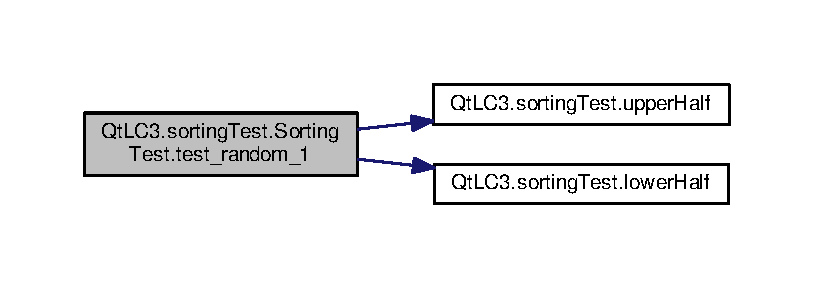
\includegraphics[width=350pt]{class_qt_l_c3_1_1sorting_test_1_1_sorting_test_a98bd681eacb66a9ed2f7ca3389c88d0c_cgraph}
\end{center}
\end{figure}




\subsection{Member Data Documentation}
\hypertarget{class_qt_l_c3_1_1sorting_test_1_1_sorting_test_a7c42c3f120e66c3a19d29aa0e4afc9ec}{\index{Qt\-L\-C3\-::sorting\-Test\-::\-Sorting\-Test@{Qt\-L\-C3\-::sorting\-Test\-::\-Sorting\-Test}!sim@{sim}}
\index{sim@{sim}!QtLC3::sortingTest::SortingTest@{Qt\-L\-C3\-::sorting\-Test\-::\-Sorting\-Test}}
\subsubsection[{sim}]{\setlength{\rightskip}{0pt plus 5cm}Qt\-L\-C3.\-sorting\-Test.\-Sorting\-Test.\-sim}}\label{class_qt_l_c3_1_1sorting_test_1_1_sorting_test_a7c42c3f120e66c3a19d29aa0e4afc9ec}


Definition at line 31 of file sorting\-Test.\-py.



The documentation for this class was generated from the following file\-:\begin{DoxyCompactItemize}
\item 
\hyperlink{sorting_test_8py}{sorting\-Test.\-py}\end{DoxyCompactItemize}

\hypertarget{classsorting_test_1_1_sorting_test}{\section{sorting\-Test.\-Sorting\-Test Class Reference}
\label{classsorting_test_1_1_sorting_test}\index{sorting\-Test.\-Sorting\-Test@{sorting\-Test.\-Sorting\-Test}}
}


Inheritance diagram for sorting\-Test.\-Sorting\-Test\-:
\nopagebreak
\begin{figure}[H]
\begin{center}
\leavevmode
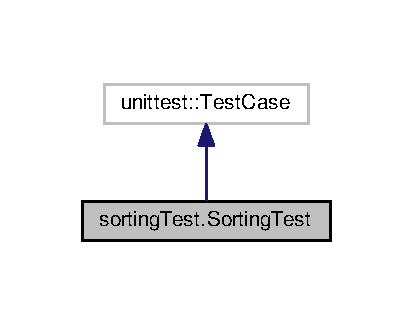
\includegraphics[width=198pt]{classsorting_test_1_1_sorting_test__inherit__graph}
\end{center}
\end{figure}


Collaboration diagram for sorting\-Test.\-Sorting\-Test\-:
\nopagebreak
\begin{figure}[H]
\begin{center}
\leavevmode
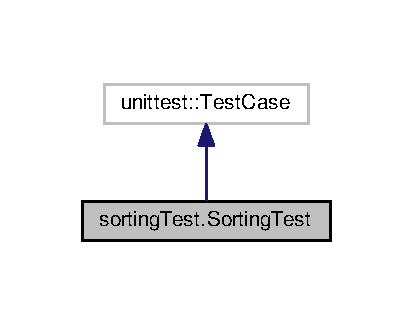
\includegraphics[width=198pt]{classsorting_test_1_1_sorting_test__coll__graph}
\end{center}
\end{figure}
\subsection*{Public Member Functions}
\begin{DoxyCompactItemize}
\item 
def \hyperlink{classsorting_test_1_1_sorting_test_af6e2aa51c92f7fa5e53338621dc4bcf5}{set\-Up}
\item 
def \hyperlink{classsorting_test_1_1_sorting_test_a711be0994263a230f34937c31923c9b2}{test\-\_\-\-Provided\-In\-Document}
\item 
def \hyperlink{classsorting_test_1_1_sorting_test_a8ebad2ff4cd9b6a96a8a975e4578b12e}{test\-\_\-random\-\_\-1}
\end{DoxyCompactItemize}
\subsection*{Public Attributes}
\begin{DoxyCompactItemize}
\item 
\hyperlink{classsorting_test_1_1_sorting_test_a2dcc99b63fb19bd7e7789303a491e784}{sim}
\end{DoxyCompactItemize}


\subsection{Detailed Description}


Definition at line 26 of file sorting\-Test.\-py.



\subsection{Member Function Documentation}
\hypertarget{classsorting_test_1_1_sorting_test_af6e2aa51c92f7fa5e53338621dc4bcf5}{\index{sorting\-Test\-::\-Sorting\-Test@{sorting\-Test\-::\-Sorting\-Test}!set\-Up@{set\-Up}}
\index{set\-Up@{set\-Up}!sortingTest::SortingTest@{sorting\-Test\-::\-Sorting\-Test}}
\subsubsection[{set\-Up}]{\setlength{\rightskip}{0pt plus 5cm}def sorting\-Test.\-Sorting\-Test.\-set\-Up (
\begin{DoxyParamCaption}
\item[{}]{self}
\end{DoxyParamCaption}
)}}\label{classsorting_test_1_1_sorting_test_af6e2aa51c92f7fa5e53338621dc4bcf5}


Definition at line 28 of file sorting\-Test.\-py.

\hypertarget{classsorting_test_1_1_sorting_test_a711be0994263a230f34937c31923c9b2}{\index{sorting\-Test\-::\-Sorting\-Test@{sorting\-Test\-::\-Sorting\-Test}!test\-\_\-\-Provided\-In\-Document@{test\-\_\-\-Provided\-In\-Document}}
\index{test\-\_\-\-Provided\-In\-Document@{test\-\_\-\-Provided\-In\-Document}!sortingTest::SortingTest@{sorting\-Test\-::\-Sorting\-Test}}
\subsubsection[{test\-\_\-\-Provided\-In\-Document}]{\setlength{\rightskip}{0pt plus 5cm}def sorting\-Test.\-Sorting\-Test.\-test\-\_\-\-Provided\-In\-Document (
\begin{DoxyParamCaption}
\item[{}]{self}
\end{DoxyParamCaption}
)}}\label{classsorting_test_1_1_sorting_test_a711be0994263a230f34937c31923c9b2}


Definition at line 33 of file sorting\-Test.\-py.



Here is the call graph for this function\-:
\nopagebreak
\begin{figure}[H]
\begin{center}
\leavevmode
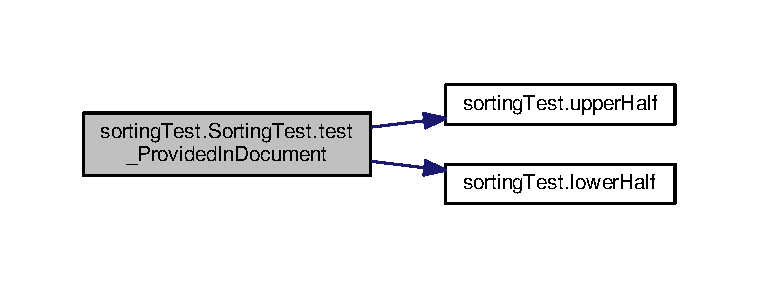
\includegraphics[width=350pt]{classsorting_test_1_1_sorting_test_a711be0994263a230f34937c31923c9b2_cgraph}
\end{center}
\end{figure}


\hypertarget{classsorting_test_1_1_sorting_test_a8ebad2ff4cd9b6a96a8a975e4578b12e}{\index{sorting\-Test\-::\-Sorting\-Test@{sorting\-Test\-::\-Sorting\-Test}!test\-\_\-random\-\_\-1@{test\-\_\-random\-\_\-1}}
\index{test\-\_\-random\-\_\-1@{test\-\_\-random\-\_\-1}!sortingTest::SortingTest@{sorting\-Test\-::\-Sorting\-Test}}
\subsubsection[{test\-\_\-random\-\_\-1}]{\setlength{\rightskip}{0pt plus 5cm}def sorting\-Test.\-Sorting\-Test.\-test\-\_\-random\-\_\-1 (
\begin{DoxyParamCaption}
\item[{}]{self}
\end{DoxyParamCaption}
)}}\label{classsorting_test_1_1_sorting_test_a8ebad2ff4cd9b6a96a8a975e4578b12e}


Definition at line 49 of file sorting\-Test.\-py.



Here is the call graph for this function\-:
\nopagebreak
\begin{figure}[H]
\begin{center}
\leavevmode
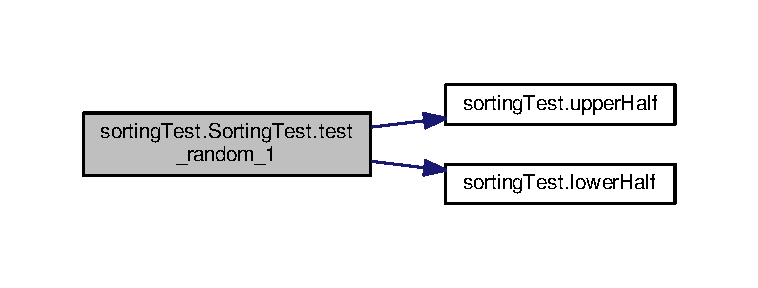
\includegraphics[width=350pt]{classsorting_test_1_1_sorting_test_a8ebad2ff4cd9b6a96a8a975e4578b12e_cgraph}
\end{center}
\end{figure}




\subsection{Member Data Documentation}
\hypertarget{classsorting_test_1_1_sorting_test_a2dcc99b63fb19bd7e7789303a491e784}{\index{sorting\-Test\-::\-Sorting\-Test@{sorting\-Test\-::\-Sorting\-Test}!sim@{sim}}
\index{sim@{sim}!sortingTest::SortingTest@{sorting\-Test\-::\-Sorting\-Test}}
\subsubsection[{sim}]{\setlength{\rightskip}{0pt plus 5cm}sorting\-Test.\-Sorting\-Test.\-sim}}\label{classsorting_test_1_1_sorting_test_a2dcc99b63fb19bd7e7789303a491e784}


Definition at line 29 of file sorting\-Test.\-py.



The documentation for this class was generated from the following file\-:\begin{DoxyCompactItemize}
\item 
grading\-\_\-sim/\hyperlink{grading__sim_2sorting_test_8py}{sorting\-Test.\-py}\end{DoxyCompactItemize}

\hypertarget{class_qt_l_c3_1_1simulator_unit_tests_1_1_test_add}{\section{Qt\-L\-C3.\-simulator\-Unit\-Tests.\-Test\-Add Class Reference}
\label{class_qt_l_c3_1_1simulator_unit_tests_1_1_test_add}\index{Qt\-L\-C3.\-simulator\-Unit\-Tests.\-Test\-Add@{Qt\-L\-C3.\-simulator\-Unit\-Tests.\-Test\-Add}}
}


Inheritance diagram for Qt\-L\-C3.\-simulator\-Unit\-Tests.\-Test\-Add\-:
\nopagebreak
\begin{figure}[H]
\begin{center}
\leavevmode
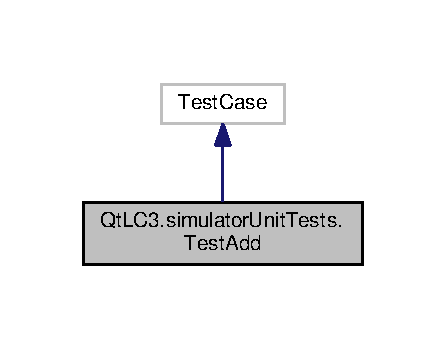
\includegraphics[width=214pt]{class_qt_l_c3_1_1simulator_unit_tests_1_1_test_add__inherit__graph}
\end{center}
\end{figure}


Collaboration diagram for Qt\-L\-C3.\-simulator\-Unit\-Tests.\-Test\-Add\-:
\nopagebreak
\begin{figure}[H]
\begin{center}
\leavevmode
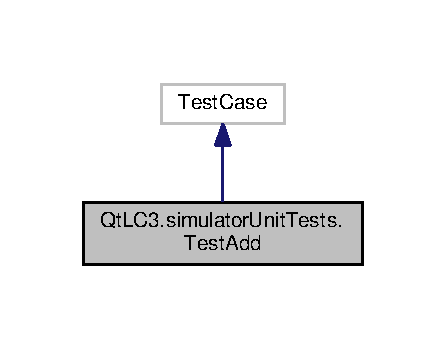
\includegraphics[width=214pt]{class_qt_l_c3_1_1simulator_unit_tests_1_1_test_add__coll__graph}
\end{center}
\end{figure}
\subsection*{Public Member Functions}
\begin{DoxyCompactItemize}
\item 
def \hyperlink{class_qt_l_c3_1_1simulator_unit_tests_1_1_test_add_aa1011545477d27c0e2e316630637a01d}{set\-Up}
\item 
def \hyperlink{class_qt_l_c3_1_1simulator_unit_tests_1_1_test_add_a26065baa41d1307e909ec88f1f769561}{test\-\_\-\-A\-D\-D\-R\-\_\-1}
\item 
def \hyperlink{class_qt_l_c3_1_1simulator_unit_tests_1_1_test_add_ae389cc6ea6673d5ca2aef3dd43077ba2}{test\-\_\-\-A\-D\-D\-R\-\_\-2}
\item 
def \hyperlink{class_qt_l_c3_1_1simulator_unit_tests_1_1_test_add_a35f45f4485e48b46d451b35d367cb636}{test\-\_\-\-A\-D\-D\-R\-\_\-3}
\item 
def \hyperlink{class_qt_l_c3_1_1simulator_unit_tests_1_1_test_add_a18567258930333030d5bd875fa4d0696}{test\-\_\-\-A\-D\-D\-I}
\end{DoxyCompactItemize}
\subsection*{Public Attributes}
\begin{DoxyCompactItemize}
\item 
\hyperlink{class_qt_l_c3_1_1simulator_unit_tests_1_1_test_add_a409a87002e770e61fc298ec7a3a1b9b3}{sim}
\end{DoxyCompactItemize}


\subsection{Detailed Description}


Definition at line 9 of file simulator\-Unit\-Tests.\-py.



\subsection{Member Function Documentation}
\hypertarget{class_qt_l_c3_1_1simulator_unit_tests_1_1_test_add_aa1011545477d27c0e2e316630637a01d}{\index{Qt\-L\-C3\-::simulator\-Unit\-Tests\-::\-Test\-Add@{Qt\-L\-C3\-::simulator\-Unit\-Tests\-::\-Test\-Add}!set\-Up@{set\-Up}}
\index{set\-Up@{set\-Up}!QtLC3::simulatorUnitTests::TestAdd@{Qt\-L\-C3\-::simulator\-Unit\-Tests\-::\-Test\-Add}}
\subsubsection[{set\-Up}]{\setlength{\rightskip}{0pt plus 5cm}def Qt\-L\-C3.\-simulator\-Unit\-Tests.\-Test\-Add.\-set\-Up (
\begin{DoxyParamCaption}
\item[{}]{self}
\end{DoxyParamCaption}
)}}\label{class_qt_l_c3_1_1simulator_unit_tests_1_1_test_add_aa1011545477d27c0e2e316630637a01d}


Definition at line 11 of file simulator\-Unit\-Tests.\-py.

\hypertarget{class_qt_l_c3_1_1simulator_unit_tests_1_1_test_add_a18567258930333030d5bd875fa4d0696}{\index{Qt\-L\-C3\-::simulator\-Unit\-Tests\-::\-Test\-Add@{Qt\-L\-C3\-::simulator\-Unit\-Tests\-::\-Test\-Add}!test\-\_\-\-A\-D\-D\-I@{test\-\_\-\-A\-D\-D\-I}}
\index{test\-\_\-\-A\-D\-D\-I@{test\-\_\-\-A\-D\-D\-I}!QtLC3::simulatorUnitTests::TestAdd@{Qt\-L\-C3\-::simulator\-Unit\-Tests\-::\-Test\-Add}}
\subsubsection[{test\-\_\-\-A\-D\-D\-I}]{\setlength{\rightskip}{0pt plus 5cm}def Qt\-L\-C3.\-simulator\-Unit\-Tests.\-Test\-Add.\-test\-\_\-\-A\-D\-D\-I (
\begin{DoxyParamCaption}
\item[{}]{self}
\end{DoxyParamCaption}
)}}\label{class_qt_l_c3_1_1simulator_unit_tests_1_1_test_add_a18567258930333030d5bd875fa4d0696}


Definition at line 42 of file simulator\-Unit\-Tests.\-py.



Here is the call graph for this function\-:
\nopagebreak
\begin{figure}[H]
\begin{center}
\leavevmode
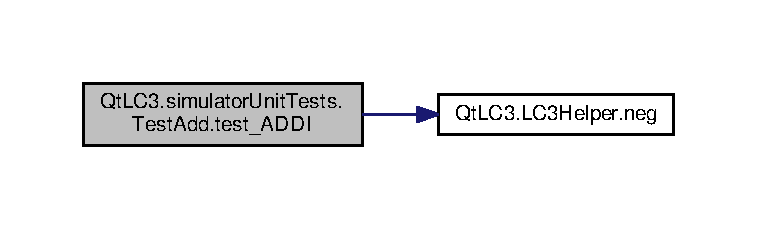
\includegraphics[width=350pt]{class_qt_l_c3_1_1simulator_unit_tests_1_1_test_add_a18567258930333030d5bd875fa4d0696_cgraph}
\end{center}
\end{figure}


\hypertarget{class_qt_l_c3_1_1simulator_unit_tests_1_1_test_add_a26065baa41d1307e909ec88f1f769561}{\index{Qt\-L\-C3\-::simulator\-Unit\-Tests\-::\-Test\-Add@{Qt\-L\-C3\-::simulator\-Unit\-Tests\-::\-Test\-Add}!test\-\_\-\-A\-D\-D\-R\-\_\-1@{test\-\_\-\-A\-D\-D\-R\-\_\-1}}
\index{test\-\_\-\-A\-D\-D\-R\-\_\-1@{test\-\_\-\-A\-D\-D\-R\-\_\-1}!QtLC3::simulatorUnitTests::TestAdd@{Qt\-L\-C3\-::simulator\-Unit\-Tests\-::\-Test\-Add}}
\subsubsection[{test\-\_\-\-A\-D\-D\-R\-\_\-1}]{\setlength{\rightskip}{0pt plus 5cm}def Qt\-L\-C3.\-simulator\-Unit\-Tests.\-Test\-Add.\-test\-\_\-\-A\-D\-D\-R\-\_\-1 (
\begin{DoxyParamCaption}
\item[{}]{self}
\end{DoxyParamCaption}
)}}\label{class_qt_l_c3_1_1simulator_unit_tests_1_1_test_add_a26065baa41d1307e909ec88f1f769561}


Definition at line 18 of file simulator\-Unit\-Tests.\-py.

\hypertarget{class_qt_l_c3_1_1simulator_unit_tests_1_1_test_add_ae389cc6ea6673d5ca2aef3dd43077ba2}{\index{Qt\-L\-C3\-::simulator\-Unit\-Tests\-::\-Test\-Add@{Qt\-L\-C3\-::simulator\-Unit\-Tests\-::\-Test\-Add}!test\-\_\-\-A\-D\-D\-R\-\_\-2@{test\-\_\-\-A\-D\-D\-R\-\_\-2}}
\index{test\-\_\-\-A\-D\-D\-R\-\_\-2@{test\-\_\-\-A\-D\-D\-R\-\_\-2}!QtLC3::simulatorUnitTests::TestAdd@{Qt\-L\-C3\-::simulator\-Unit\-Tests\-::\-Test\-Add}}
\subsubsection[{test\-\_\-\-A\-D\-D\-R\-\_\-2}]{\setlength{\rightskip}{0pt plus 5cm}def Qt\-L\-C3.\-simulator\-Unit\-Tests.\-Test\-Add.\-test\-\_\-\-A\-D\-D\-R\-\_\-2 (
\begin{DoxyParamCaption}
\item[{}]{self}
\end{DoxyParamCaption}
)}}\label{class_qt_l_c3_1_1simulator_unit_tests_1_1_test_add_ae389cc6ea6673d5ca2aef3dd43077ba2}


Definition at line 26 of file simulator\-Unit\-Tests.\-py.



Here is the call graph for this function\-:
\nopagebreak
\begin{figure}[H]
\begin{center}
\leavevmode
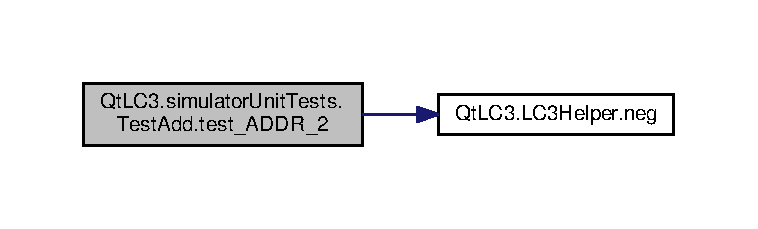
\includegraphics[width=350pt]{class_qt_l_c3_1_1simulator_unit_tests_1_1_test_add_ae389cc6ea6673d5ca2aef3dd43077ba2_cgraph}
\end{center}
\end{figure}


\hypertarget{class_qt_l_c3_1_1simulator_unit_tests_1_1_test_add_a35f45f4485e48b46d451b35d367cb636}{\index{Qt\-L\-C3\-::simulator\-Unit\-Tests\-::\-Test\-Add@{Qt\-L\-C3\-::simulator\-Unit\-Tests\-::\-Test\-Add}!test\-\_\-\-A\-D\-D\-R\-\_\-3@{test\-\_\-\-A\-D\-D\-R\-\_\-3}}
\index{test\-\_\-\-A\-D\-D\-R\-\_\-3@{test\-\_\-\-A\-D\-D\-R\-\_\-3}!QtLC3::simulatorUnitTests::TestAdd@{Qt\-L\-C3\-::simulator\-Unit\-Tests\-::\-Test\-Add}}
\subsubsection[{test\-\_\-\-A\-D\-D\-R\-\_\-3}]{\setlength{\rightskip}{0pt plus 5cm}def Qt\-L\-C3.\-simulator\-Unit\-Tests.\-Test\-Add.\-test\-\_\-\-A\-D\-D\-R\-\_\-3 (
\begin{DoxyParamCaption}
\item[{}]{self}
\end{DoxyParamCaption}
)}}\label{class_qt_l_c3_1_1simulator_unit_tests_1_1_test_add_a35f45f4485e48b46d451b35d367cb636}


Definition at line 33 of file simulator\-Unit\-Tests.\-py.



\subsection{Member Data Documentation}
\hypertarget{class_qt_l_c3_1_1simulator_unit_tests_1_1_test_add_a409a87002e770e61fc298ec7a3a1b9b3}{\index{Qt\-L\-C3\-::simulator\-Unit\-Tests\-::\-Test\-Add@{Qt\-L\-C3\-::simulator\-Unit\-Tests\-::\-Test\-Add}!sim@{sim}}
\index{sim@{sim}!QtLC3::simulatorUnitTests::TestAdd@{Qt\-L\-C3\-::simulator\-Unit\-Tests\-::\-Test\-Add}}
\subsubsection[{sim}]{\setlength{\rightskip}{0pt plus 5cm}Qt\-L\-C3.\-simulator\-Unit\-Tests.\-Test\-Add.\-sim}}\label{class_qt_l_c3_1_1simulator_unit_tests_1_1_test_add_a409a87002e770e61fc298ec7a3a1b9b3}


Definition at line 12 of file simulator\-Unit\-Tests.\-py.



The documentation for this class was generated from the following file\-:\begin{DoxyCompactItemize}
\item 
\hyperlink{simulator_unit_tests_8py}{simulator\-Unit\-Tests.\-py}\end{DoxyCompactItemize}

\hypertarget{class_qt_l_c3_1_1simulator_unit_tests_1_1_test_and}{\section{Qt\-L\-C3.\-simulator\-Unit\-Tests.\-Test\-And Class Reference}
\label{class_qt_l_c3_1_1simulator_unit_tests_1_1_test_and}\index{Qt\-L\-C3.\-simulator\-Unit\-Tests.\-Test\-And@{Qt\-L\-C3.\-simulator\-Unit\-Tests.\-Test\-And}}
}


Inheritance diagram for Qt\-L\-C3.\-simulator\-Unit\-Tests.\-Test\-And\-:
\nopagebreak
\begin{figure}[H]
\begin{center}
\leavevmode
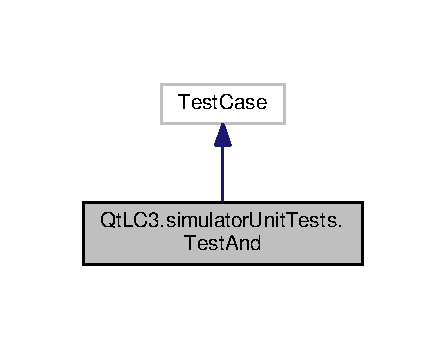
\includegraphics[width=214pt]{class_qt_l_c3_1_1simulator_unit_tests_1_1_test_and__inherit__graph}
\end{center}
\end{figure}


Collaboration diagram for Qt\-L\-C3.\-simulator\-Unit\-Tests.\-Test\-And\-:
\nopagebreak
\begin{figure}[H]
\begin{center}
\leavevmode
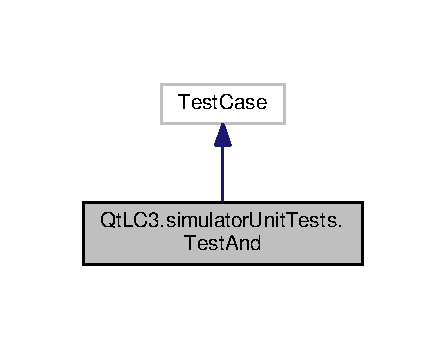
\includegraphics[width=214pt]{class_qt_l_c3_1_1simulator_unit_tests_1_1_test_and__coll__graph}
\end{center}
\end{figure}
\subsection*{Public Member Functions}
\begin{DoxyCompactItemize}
\item 
def \hyperlink{class_qt_l_c3_1_1simulator_unit_tests_1_1_test_and_ab75b9a12a4a12cf9e6ee9b26f809d8ed}{set\-Up}
\item 
def \hyperlink{class_qt_l_c3_1_1simulator_unit_tests_1_1_test_and_ac5327caa08d5c3ad3dc54e51493a3313}{test\-\_\-\-A\-N\-D1}
\item 
def \hyperlink{class_qt_l_c3_1_1simulator_unit_tests_1_1_test_and_ac5327caa08d5c3ad3dc54e51493a3313}{test\-\_\-\-A\-N\-D1}
\item 
def \hyperlink{class_qt_l_c3_1_1simulator_unit_tests_1_1_test_and_ac5327caa08d5c3ad3dc54e51493a3313}{test\-\_\-\-A\-N\-D1}
\end{DoxyCompactItemize}
\subsection*{Public Attributes}
\begin{DoxyCompactItemize}
\item 
\hyperlink{class_qt_l_c3_1_1simulator_unit_tests_1_1_test_and_abfd247caf206df6fe94b24b0deb32469}{sim}
\end{DoxyCompactItemize}


\subsection{Detailed Description}


Definition at line 62 of file simulator\-Unit\-Tests.\-py.



\subsection{Member Function Documentation}
\hypertarget{class_qt_l_c3_1_1simulator_unit_tests_1_1_test_and_ab75b9a12a4a12cf9e6ee9b26f809d8ed}{\index{Qt\-L\-C3\-::simulator\-Unit\-Tests\-::\-Test\-And@{Qt\-L\-C3\-::simulator\-Unit\-Tests\-::\-Test\-And}!set\-Up@{set\-Up}}
\index{set\-Up@{set\-Up}!QtLC3::simulatorUnitTests::TestAnd@{Qt\-L\-C3\-::simulator\-Unit\-Tests\-::\-Test\-And}}
\subsubsection[{set\-Up}]{\setlength{\rightskip}{0pt plus 5cm}def Qt\-L\-C3.\-simulator\-Unit\-Tests.\-Test\-And.\-set\-Up (
\begin{DoxyParamCaption}
\item[{}]{self}
\end{DoxyParamCaption}
)}}\label{class_qt_l_c3_1_1simulator_unit_tests_1_1_test_and_ab75b9a12a4a12cf9e6ee9b26f809d8ed}


Definition at line 63 of file simulator\-Unit\-Tests.\-py.

\hypertarget{class_qt_l_c3_1_1simulator_unit_tests_1_1_test_and_ac5327caa08d5c3ad3dc54e51493a3313}{\index{Qt\-L\-C3\-::simulator\-Unit\-Tests\-::\-Test\-And@{Qt\-L\-C3\-::simulator\-Unit\-Tests\-::\-Test\-And}!test\-\_\-\-A\-N\-D1@{test\-\_\-\-A\-N\-D1}}
\index{test\-\_\-\-A\-N\-D1@{test\-\_\-\-A\-N\-D1}!QtLC3::simulatorUnitTests::TestAnd@{Qt\-L\-C3\-::simulator\-Unit\-Tests\-::\-Test\-And}}
\subsubsection[{test\-\_\-\-A\-N\-D1}]{\setlength{\rightskip}{0pt plus 5cm}def Qt\-L\-C3.\-simulator\-Unit\-Tests.\-Test\-And.\-test\-\_\-\-A\-N\-D1 (
\begin{DoxyParamCaption}
\item[{}]{self}
\end{DoxyParamCaption}
)}}\label{class_qt_l_c3_1_1simulator_unit_tests_1_1_test_and_ac5327caa08d5c3ad3dc54e51493a3313}


Definition at line 72 of file simulator\-Unit\-Tests.\-py.



Here is the caller graph for this function\-:
\nopagebreak
\begin{figure}[H]
\begin{center}
\leavevmode
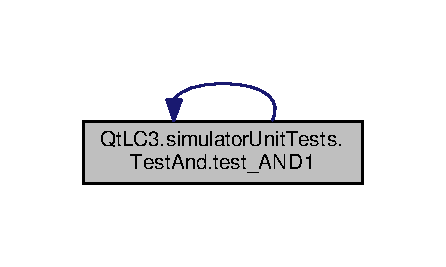
\includegraphics[width=214pt]{class_qt_l_c3_1_1simulator_unit_tests_1_1_test_and_ac5327caa08d5c3ad3dc54e51493a3313_icgraph}
\end{center}
\end{figure}


\hypertarget{class_qt_l_c3_1_1simulator_unit_tests_1_1_test_and_ac5327caa08d5c3ad3dc54e51493a3313}{\index{Qt\-L\-C3\-::simulator\-Unit\-Tests\-::\-Test\-And@{Qt\-L\-C3\-::simulator\-Unit\-Tests\-::\-Test\-And}!test\-\_\-\-A\-N\-D1@{test\-\_\-\-A\-N\-D1}}
\index{test\-\_\-\-A\-N\-D1@{test\-\_\-\-A\-N\-D1}!QtLC3::simulatorUnitTests::TestAnd@{Qt\-L\-C3\-::simulator\-Unit\-Tests\-::\-Test\-And}}
\subsubsection[{test\-\_\-\-A\-N\-D1}]{\setlength{\rightskip}{0pt plus 5cm}def Qt\-L\-C3.\-simulator\-Unit\-Tests.\-Test\-And.\-test\-\_\-\-A\-N\-D1 (
\begin{DoxyParamCaption}
\item[{}]{self}
\end{DoxyParamCaption}
)}}\label{class_qt_l_c3_1_1simulator_unit_tests_1_1_test_and_ac5327caa08d5c3ad3dc54e51493a3313}


Definition at line 79 of file simulator\-Unit\-Tests.\-py.



Here is the call graph for this function\-:
\nopagebreak
\begin{figure}[H]
\begin{center}
\leavevmode
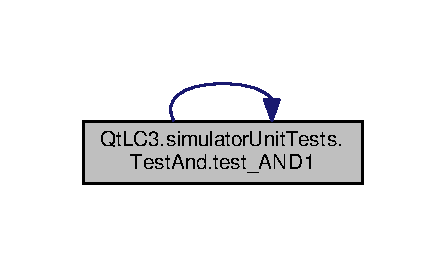
\includegraphics[width=214pt]{class_qt_l_c3_1_1simulator_unit_tests_1_1_test_and_ac5327caa08d5c3ad3dc54e51493a3313_cgraph}
\end{center}
\end{figure}


\hypertarget{class_qt_l_c3_1_1simulator_unit_tests_1_1_test_and_ac5327caa08d5c3ad3dc54e51493a3313}{\index{Qt\-L\-C3\-::simulator\-Unit\-Tests\-::\-Test\-And@{Qt\-L\-C3\-::simulator\-Unit\-Tests\-::\-Test\-And}!test\-\_\-\-A\-N\-D1@{test\-\_\-\-A\-N\-D1}}
\index{test\-\_\-\-A\-N\-D1@{test\-\_\-\-A\-N\-D1}!QtLC3::simulatorUnitTests::TestAnd@{Qt\-L\-C3\-::simulator\-Unit\-Tests\-::\-Test\-And}}
\subsubsection[{test\-\_\-\-A\-N\-D1}]{\setlength{\rightskip}{0pt plus 5cm}def Qt\-L\-C3.\-simulator\-Unit\-Tests.\-Test\-And.\-test\-\_\-\-A\-N\-D1 (
\begin{DoxyParamCaption}
\item[{}]{self}
\end{DoxyParamCaption}
)}}\label{class_qt_l_c3_1_1simulator_unit_tests_1_1_test_and_ac5327caa08d5c3ad3dc54e51493a3313}


Definition at line 86 of file simulator\-Unit\-Tests.\-py.



Here is the call graph for this function\-:
\nopagebreak
\begin{figure}[H]
\begin{center}
\leavevmode
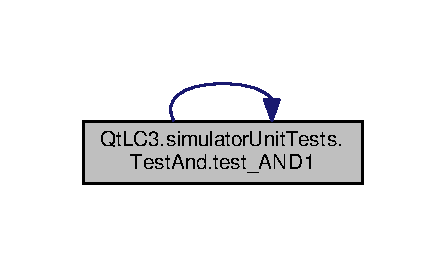
\includegraphics[width=214pt]{class_qt_l_c3_1_1simulator_unit_tests_1_1_test_and_ac5327caa08d5c3ad3dc54e51493a3313_cgraph}
\end{center}
\end{figure}




\subsection{Member Data Documentation}
\hypertarget{class_qt_l_c3_1_1simulator_unit_tests_1_1_test_and_abfd247caf206df6fe94b24b0deb32469}{\index{Qt\-L\-C3\-::simulator\-Unit\-Tests\-::\-Test\-And@{Qt\-L\-C3\-::simulator\-Unit\-Tests\-::\-Test\-And}!sim@{sim}}
\index{sim@{sim}!QtLC3::simulatorUnitTests::TestAnd@{Qt\-L\-C3\-::simulator\-Unit\-Tests\-::\-Test\-And}}
\subsubsection[{sim}]{\setlength{\rightskip}{0pt plus 5cm}Qt\-L\-C3.\-simulator\-Unit\-Tests.\-Test\-And.\-sim}}\label{class_qt_l_c3_1_1simulator_unit_tests_1_1_test_and_abfd247caf206df6fe94b24b0deb32469}


Definition at line 65 of file simulator\-Unit\-Tests.\-py.



The documentation for this class was generated from the following file\-:\begin{DoxyCompactItemize}
\item 
\hyperlink{simulator_unit_tests_8py}{simulator\-Unit\-Tests.\-py}\end{DoxyCompactItemize}

\hypertarget{class_qt_l_c3_1_1simulator_unit_tests_1_1_test_watch_point}{\section{Qt\-L\-C3.\-simulator\-Unit\-Tests.\-Test\-Watch\-Point Class Reference}
\label{class_qt_l_c3_1_1simulator_unit_tests_1_1_test_watch_point}\index{Qt\-L\-C3.\-simulator\-Unit\-Tests.\-Test\-Watch\-Point@{Qt\-L\-C3.\-simulator\-Unit\-Tests.\-Test\-Watch\-Point}}
}


Inheritance diagram for Qt\-L\-C3.\-simulator\-Unit\-Tests.\-Test\-Watch\-Point\-:
\nopagebreak
\begin{figure}[H]
\begin{center}
\leavevmode
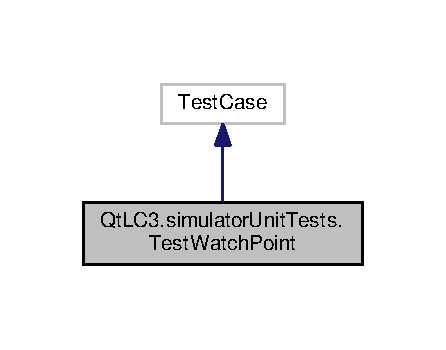
\includegraphics[width=214pt]{class_qt_l_c3_1_1simulator_unit_tests_1_1_test_watch_point__inherit__graph}
\end{center}
\end{figure}


Collaboration diagram for Qt\-L\-C3.\-simulator\-Unit\-Tests.\-Test\-Watch\-Point\-:
\nopagebreak
\begin{figure}[H]
\begin{center}
\leavevmode
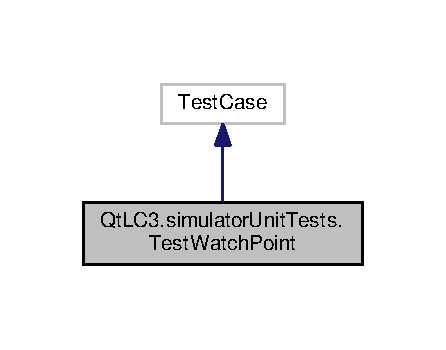
\includegraphics[width=214pt]{class_qt_l_c3_1_1simulator_unit_tests_1_1_test_watch_point__coll__graph}
\end{center}
\end{figure}
\subsection*{Public Member Functions}
\begin{DoxyCompactItemize}
\item 
def \hyperlink{class_qt_l_c3_1_1simulator_unit_tests_1_1_test_watch_point_ae07fb07e4c1038024bfb0f479e600e7c}{set\-Up}
\item 
def \hyperlink{class_qt_l_c3_1_1simulator_unit_tests_1_1_test_watch_point_aead000bd3cddde7913b55a23222f1ad8}{test\-\_\-\-Watch\-Read}
\item 
def \hyperlink{class_qt_l_c3_1_1simulator_unit_tests_1_1_test_watch_point_aec0f9b981b4e3e1cd31085b522d8bc72}{test\-\_\-\-Watch\-Write}
\item 
def \hyperlink{class_qt_l_c3_1_1simulator_unit_tests_1_1_test_watch_point_a70c348480ac97396b9e5d1889f374692}{test\-\_\-\-Watch\-Read\-Write}
\end{DoxyCompactItemize}
\subsection*{Public Attributes}
\begin{DoxyCompactItemize}
\item 
\hyperlink{class_qt_l_c3_1_1simulator_unit_tests_1_1_test_watch_point_ae94aeccff41200c0de16ec2002cc2a18}{sim}
\item 
\hyperlink{class_qt_l_c3_1_1simulator_unit_tests_1_1_test_watch_point_a650cf940e4a573cf7a06561942e33f5f}{called}
\end{DoxyCompactItemize}


\subsection{Detailed Description}


Definition at line 93 of file simulator\-Unit\-Tests.\-py.



\subsection{Member Function Documentation}
\hypertarget{class_qt_l_c3_1_1simulator_unit_tests_1_1_test_watch_point_ae07fb07e4c1038024bfb0f479e600e7c}{\index{Qt\-L\-C3\-::simulator\-Unit\-Tests\-::\-Test\-Watch\-Point@{Qt\-L\-C3\-::simulator\-Unit\-Tests\-::\-Test\-Watch\-Point}!set\-Up@{set\-Up}}
\index{set\-Up@{set\-Up}!QtLC3::simulatorUnitTests::TestWatchPoint@{Qt\-L\-C3\-::simulator\-Unit\-Tests\-::\-Test\-Watch\-Point}}
\subsubsection[{set\-Up}]{\setlength{\rightskip}{0pt plus 5cm}def Qt\-L\-C3.\-simulator\-Unit\-Tests.\-Test\-Watch\-Point.\-set\-Up (
\begin{DoxyParamCaption}
\item[{}]{self}
\end{DoxyParamCaption}
)}}\label{class_qt_l_c3_1_1simulator_unit_tests_1_1_test_watch_point_ae07fb07e4c1038024bfb0f479e600e7c}


Definition at line 94 of file simulator\-Unit\-Tests.\-py.

\hypertarget{class_qt_l_c3_1_1simulator_unit_tests_1_1_test_watch_point_aead000bd3cddde7913b55a23222f1ad8}{\index{Qt\-L\-C3\-::simulator\-Unit\-Tests\-::\-Test\-Watch\-Point@{Qt\-L\-C3\-::simulator\-Unit\-Tests\-::\-Test\-Watch\-Point}!test\-\_\-\-Watch\-Read@{test\-\_\-\-Watch\-Read}}
\index{test\-\_\-\-Watch\-Read@{test\-\_\-\-Watch\-Read}!QtLC3::simulatorUnitTests::TestWatchPoint@{Qt\-L\-C3\-::simulator\-Unit\-Tests\-::\-Test\-Watch\-Point}}
\subsubsection[{test\-\_\-\-Watch\-Read}]{\setlength{\rightskip}{0pt plus 5cm}def Qt\-L\-C3.\-simulator\-Unit\-Tests.\-Test\-Watch\-Point.\-test\-\_\-\-Watch\-Read (
\begin{DoxyParamCaption}
\item[{}]{self}
\end{DoxyParamCaption}
)}}\label{class_qt_l_c3_1_1simulator_unit_tests_1_1_test_watch_point_aead000bd3cddde7913b55a23222f1ad8}


Definition at line 97 of file simulator\-Unit\-Tests.\-py.

\hypertarget{class_qt_l_c3_1_1simulator_unit_tests_1_1_test_watch_point_a70c348480ac97396b9e5d1889f374692}{\index{Qt\-L\-C3\-::simulator\-Unit\-Tests\-::\-Test\-Watch\-Point@{Qt\-L\-C3\-::simulator\-Unit\-Tests\-::\-Test\-Watch\-Point}!test\-\_\-\-Watch\-Read\-Write@{test\-\_\-\-Watch\-Read\-Write}}
\index{test\-\_\-\-Watch\-Read\-Write@{test\-\_\-\-Watch\-Read\-Write}!QtLC3::simulatorUnitTests::TestWatchPoint@{Qt\-L\-C3\-::simulator\-Unit\-Tests\-::\-Test\-Watch\-Point}}
\subsubsection[{test\-\_\-\-Watch\-Read\-Write}]{\setlength{\rightskip}{0pt plus 5cm}def Qt\-L\-C3.\-simulator\-Unit\-Tests.\-Test\-Watch\-Point.\-test\-\_\-\-Watch\-Read\-Write (
\begin{DoxyParamCaption}
\item[{}]{self}
\end{DoxyParamCaption}
)}}\label{class_qt_l_c3_1_1simulator_unit_tests_1_1_test_watch_point_a70c348480ac97396b9e5d1889f374692}


Definition at line 127 of file simulator\-Unit\-Tests.\-py.



Here is the call graph for this function\-:
\nopagebreak
\begin{figure}[H]
\begin{center}
\leavevmode
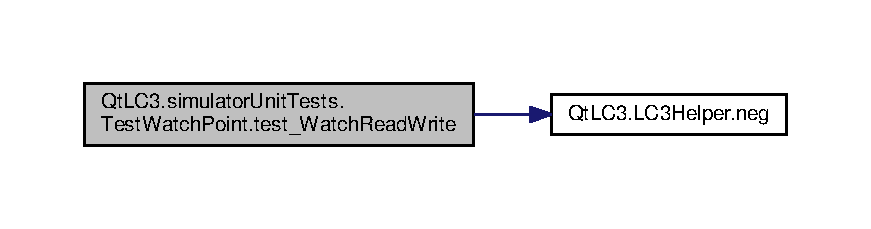
\includegraphics[width=350pt]{class_qt_l_c3_1_1simulator_unit_tests_1_1_test_watch_point_a70c348480ac97396b9e5d1889f374692_cgraph}
\end{center}
\end{figure}


\hypertarget{class_qt_l_c3_1_1simulator_unit_tests_1_1_test_watch_point_aec0f9b981b4e3e1cd31085b522d8bc72}{\index{Qt\-L\-C3\-::simulator\-Unit\-Tests\-::\-Test\-Watch\-Point@{Qt\-L\-C3\-::simulator\-Unit\-Tests\-::\-Test\-Watch\-Point}!test\-\_\-\-Watch\-Write@{test\-\_\-\-Watch\-Write}}
\index{test\-\_\-\-Watch\-Write@{test\-\_\-\-Watch\-Write}!QtLC3::simulatorUnitTests::TestWatchPoint@{Qt\-L\-C3\-::simulator\-Unit\-Tests\-::\-Test\-Watch\-Point}}
\subsubsection[{test\-\_\-\-Watch\-Write}]{\setlength{\rightskip}{0pt plus 5cm}def Qt\-L\-C3.\-simulator\-Unit\-Tests.\-Test\-Watch\-Point.\-test\-\_\-\-Watch\-Write (
\begin{DoxyParamCaption}
\item[{}]{self}
\end{DoxyParamCaption}
)}}\label{class_qt_l_c3_1_1simulator_unit_tests_1_1_test_watch_point_aec0f9b981b4e3e1cd31085b522d8bc72}


Definition at line 112 of file simulator\-Unit\-Tests.\-py.



Here is the call graph for this function\-:
\nopagebreak
\begin{figure}[H]
\begin{center}
\leavevmode
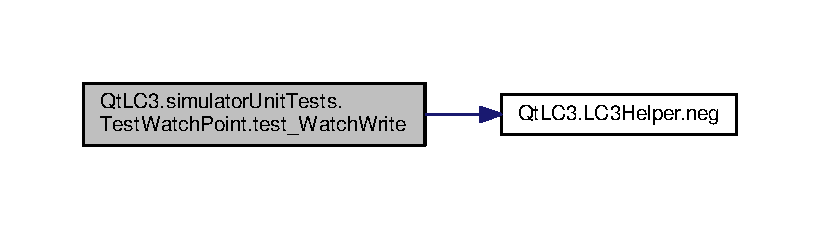
\includegraphics[width=350pt]{class_qt_l_c3_1_1simulator_unit_tests_1_1_test_watch_point_aec0f9b981b4e3e1cd31085b522d8bc72_cgraph}
\end{center}
\end{figure}




\subsection{Member Data Documentation}
\hypertarget{class_qt_l_c3_1_1simulator_unit_tests_1_1_test_watch_point_a650cf940e4a573cf7a06561942e33f5f}{\index{Qt\-L\-C3\-::simulator\-Unit\-Tests\-::\-Test\-Watch\-Point@{Qt\-L\-C3\-::simulator\-Unit\-Tests\-::\-Test\-Watch\-Point}!called@{called}}
\index{called@{called}!QtLC3::simulatorUnitTests::TestWatchPoint@{Qt\-L\-C3\-::simulator\-Unit\-Tests\-::\-Test\-Watch\-Point}}
\subsubsection[{called}]{\setlength{\rightskip}{0pt plus 5cm}Qt\-L\-C3.\-simulator\-Unit\-Tests.\-Test\-Watch\-Point.\-called}}\label{class_qt_l_c3_1_1simulator_unit_tests_1_1_test_watch_point_a650cf940e4a573cf7a06561942e33f5f}


Definition at line 98 of file simulator\-Unit\-Tests.\-py.

\hypertarget{class_qt_l_c3_1_1simulator_unit_tests_1_1_test_watch_point_ae94aeccff41200c0de16ec2002cc2a18}{\index{Qt\-L\-C3\-::simulator\-Unit\-Tests\-::\-Test\-Watch\-Point@{Qt\-L\-C3\-::simulator\-Unit\-Tests\-::\-Test\-Watch\-Point}!sim@{sim}}
\index{sim@{sim}!QtLC3::simulatorUnitTests::TestWatchPoint@{Qt\-L\-C3\-::simulator\-Unit\-Tests\-::\-Test\-Watch\-Point}}
\subsubsection[{sim}]{\setlength{\rightskip}{0pt plus 5cm}Qt\-L\-C3.\-simulator\-Unit\-Tests.\-Test\-Watch\-Point.\-sim}}\label{class_qt_l_c3_1_1simulator_unit_tests_1_1_test_watch_point_ae94aeccff41200c0de16ec2002cc2a18}


Definition at line 95 of file simulator\-Unit\-Tests.\-py.



The documentation for this class was generated from the following file\-:\begin{DoxyCompactItemize}
\item 
\hyperlink{simulator_unit_tests_8py}{simulator\-Unit\-Tests.\-py}\end{DoxyCompactItemize}

\hypertarget{struct_watch_point}{\section{Watch\-Point Struct Reference}
\label{struct_watch_point}\index{Watch\-Point@{Watch\-Point}}
}


{\ttfamily \#include $<$simulator.\-hpp$>$}

\subsection*{Public Attributes}
\begin{DoxyCompactItemize}
\item 
uint16\-\_\-t \hyperlink{struct_watch_point_a6a06d058cfef3dcf884cb9b450336e2b}{address}
\item 
uint16\-\_\-t \hyperlink{struct_watch_point_a10522099ca18d8990ed7271eea8ebe9b}{prev\-Val}
\item 
uint16\-\_\-t \hyperlink{struct_watch_point_a034305370c1f202264bde15517161c84}{curr\-Val}
\item 
bool \hyperlink{struct_watch_point_a861bd06fdc7d1344facc41e7c338eb0a}{read\-Point}
\item 
bool \hyperlink{struct_watch_point_ace0077dc7681695fdb7fbc3e44637038}{write\-Point}
\item 
Py\-Object $\ast$ \hyperlink{struct_watch_point_a5f41744f900b3b33e6585bb906e8da25}{cb}
\end{DoxyCompactItemize}


\subsection{Detailed Description}


Definition at line 18 of file simulator.\-hpp.



\subsection{Member Data Documentation}
\hypertarget{struct_watch_point_a6a06d058cfef3dcf884cb9b450336e2b}{\index{Watch\-Point@{Watch\-Point}!address@{address}}
\index{address@{address}!WatchPoint@{Watch\-Point}}
\subsubsection[{address}]{\setlength{\rightskip}{0pt plus 5cm}uint16\-\_\-t Watch\-Point\-::address}}\label{struct_watch_point_a6a06d058cfef3dcf884cb9b450336e2b}


Definition at line 19 of file simulator.\-hpp.

\hypertarget{struct_watch_point_a5f41744f900b3b33e6585bb906e8da25}{\index{Watch\-Point@{Watch\-Point}!cb@{cb}}
\index{cb@{cb}!WatchPoint@{Watch\-Point}}
\subsubsection[{cb}]{\setlength{\rightskip}{0pt plus 5cm}Py\-Object$\ast$ Watch\-Point\-::cb}}\label{struct_watch_point_a5f41744f900b3b33e6585bb906e8da25}


Definition at line 24 of file simulator.\-hpp.

\hypertarget{struct_watch_point_a034305370c1f202264bde15517161c84}{\index{Watch\-Point@{Watch\-Point}!curr\-Val@{curr\-Val}}
\index{curr\-Val@{curr\-Val}!WatchPoint@{Watch\-Point}}
\subsubsection[{curr\-Val}]{\setlength{\rightskip}{0pt plus 5cm}uint16\-\_\-t Watch\-Point\-::curr\-Val}}\label{struct_watch_point_a034305370c1f202264bde15517161c84}


Definition at line 21 of file simulator.\-hpp.

\hypertarget{struct_watch_point_a10522099ca18d8990ed7271eea8ebe9b}{\index{Watch\-Point@{Watch\-Point}!prev\-Val@{prev\-Val}}
\index{prev\-Val@{prev\-Val}!WatchPoint@{Watch\-Point}}
\subsubsection[{prev\-Val}]{\setlength{\rightskip}{0pt plus 5cm}uint16\-\_\-t Watch\-Point\-::prev\-Val}}\label{struct_watch_point_a10522099ca18d8990ed7271eea8ebe9b}


Definition at line 20 of file simulator.\-hpp.

\hypertarget{struct_watch_point_a861bd06fdc7d1344facc41e7c338eb0a}{\index{Watch\-Point@{Watch\-Point}!read\-Point@{read\-Point}}
\index{read\-Point@{read\-Point}!WatchPoint@{Watch\-Point}}
\subsubsection[{read\-Point}]{\setlength{\rightskip}{0pt plus 5cm}bool Watch\-Point\-::read\-Point}}\label{struct_watch_point_a861bd06fdc7d1344facc41e7c338eb0a}


Definition at line 22 of file simulator.\-hpp.

\hypertarget{struct_watch_point_ace0077dc7681695fdb7fbc3e44637038}{\index{Watch\-Point@{Watch\-Point}!write\-Point@{write\-Point}}
\index{write\-Point@{write\-Point}!WatchPoint@{Watch\-Point}}
\subsubsection[{write\-Point}]{\setlength{\rightskip}{0pt plus 5cm}bool Watch\-Point\-::write\-Point}}\label{struct_watch_point_ace0077dc7681695fdb7fbc3e44637038}


Definition at line 23 of file simulator.\-hpp.



The documentation for this struct was generated from the following file\-:\begin{DoxyCompactItemize}
\item 
\hyperlink{simulator_8hpp}{simulator.\-hpp}\end{DoxyCompactItemize}

\chapter{File Documentation}
\hypertarget{____init_____8py}{\section{\-\_\-\-\_\-init\-\_\-\-\_\-.\-py File Reference}
\label{____init_____8py}\index{\-\_\-\-\_\-init\-\_\-\-\_\-.\-py@{\-\_\-\-\_\-init\-\_\-\-\_\-.\-py}}
}
\subsection*{Namespaces}
\begin{DoxyCompactItemize}
\item 
\hyperlink{namespace_qt_l_c3}{Qt\-L\-C3}
\end{DoxyCompactItemize}

\hypertarget{prog__options__test1_8cpp}{\section{C\-L\-I/prog\-\_\-options\-\_\-test1.cpp File Reference}
\label{prog__options__test1_8cpp}\index{C\-L\-I/prog\-\_\-options\-\_\-test1.\-cpp@{C\-L\-I/prog\-\_\-options\-\_\-test1.\-cpp}}
}
{\ttfamily \#include \char`\"{}boost/program\-\_\-options.\-hpp\char`\"{}}\\*
{\ttfamily \#include \char`\"{}boost/filesystem.\-hpp\char`\"{}}\\*
{\ttfamily \#include $<$iostream$>$}\\*
{\ttfamily \#include $<$string$>$}\\*
Include dependency graph for prog\-\_\-options\-\_\-test1.\-cpp\-:
\nopagebreak
\begin{figure}[H]
\begin{center}
\leavevmode
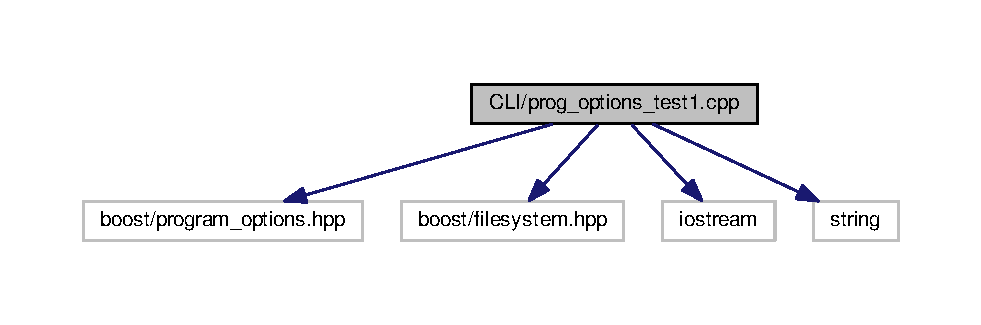
\includegraphics[width=350pt]{prog__options__test1_8cpp__incl}
\end{center}
\end{figure}
\subsection*{Functions}
\begin{DoxyCompactItemize}
\item 
int \hyperlink{prog__options__test1_8cpp_a3c04138a5bfe5d72780bb7e82a18e627}{main} (int argc, char $\ast$$\ast$argv)
\end{DoxyCompactItemize}


\subsection{Function Documentation}
\hypertarget{prog__options__test1_8cpp_a3c04138a5bfe5d72780bb7e82a18e627}{\index{prog\-\_\-options\-\_\-test1.\-cpp@{prog\-\_\-options\-\_\-test1.\-cpp}!main@{main}}
\index{main@{main}!prog_options_test1.cpp@{prog\-\_\-options\-\_\-test1.\-cpp}}
\subsubsection[{main}]{\setlength{\rightskip}{0pt plus 5cm}int main (
\begin{DoxyParamCaption}
\item[{int}]{argc, }
\item[{char $\ast$$\ast$}]{argv}
\end{DoxyParamCaption}
)}}\label{prog__options__test1_8cpp_a3c04138a5bfe5d72780bb7e82a18e627}
Define and parse the program options

--help option

Definition at line 17 of file prog\-\_\-options\-\_\-test1.\-cpp.


\hypertarget{grader_8py}{\section{grader.\-py File Reference}
\label{grader_8py}\index{grader.\-py@{grader.\-py}}
}
\subsection*{Namespaces}
\begin{DoxyCompactItemize}
\item 
\hyperlink{namespace_qt_l_c3_1_1grader}{Qt\-L\-C3.\-grader}
\end{DoxyCompactItemize}
\subsection*{Functions}
\begin{DoxyCompactItemize}
\item 
def \hyperlink{namespace_qt_l_c3_1_1grader_ac13afb6c069c67f0157826b184c11762}{Qt\-L\-C3.\-grader.\-do\-Test}
\end{DoxyCompactItemize}

\hypertarget{grading__sim_2sorting_test_8py}{\section{grading\-\_\-sim/sorting\-Test.py File Reference}
\label{grading__sim_2sorting_test_8py}\index{grading\-\_\-sim/sorting\-Test.\-py@{grading\-\_\-sim/sorting\-Test.\-py}}
}
\subsection*{Classes}
\begin{DoxyCompactItemize}
\item 
class \hyperlink{classsorting_test_1_1_sorting_test}{sorting\-Test.\-Sorting\-Test}
\end{DoxyCompactItemize}
\subsection*{Namespaces}
\begin{DoxyCompactItemize}
\item 
\hyperlink{namespacesorting_test}{sorting\-Test}
\end{DoxyCompactItemize}
\subsection*{Functions}
\begin{DoxyCompactItemize}
\item 
def \hyperlink{namespacesorting_test_a053e72abcbfaaa5a0a3ce799a4e820f7}{sorting\-Test.\-upper\-Half}
\item 
def \hyperlink{namespacesorting_test_a6c56b012d5be2f3958634adfabd4ee6e}{sorting\-Test.\-lower\-Half}
\end{DoxyCompactItemize}

\hypertarget{sorting_test_8py}{\section{sorting\-Test.\-py File Reference}
\label{sorting_test_8py}\index{sorting\-Test.\-py@{sorting\-Test.\-py}}
}
\subsection*{Classes}
\begin{DoxyCompactItemize}
\item 
class \hyperlink{class_qt_l_c3_1_1sorting_test_1_1_sorting_test}{Qt\-L\-C3.\-sorting\-Test.\-Sorting\-Test}
\end{DoxyCompactItemize}
\subsection*{Namespaces}
\begin{DoxyCompactItemize}
\item 
\hyperlink{namespace_qt_l_c3_1_1sorting_test}{Qt\-L\-C3.\-sorting\-Test}
\end{DoxyCompactItemize}
\subsection*{Functions}
\begin{DoxyCompactItemize}
\item 
def \hyperlink{namespace_qt_l_c3_1_1sorting_test_a60151bfd7e175f8f0c56327890bf6de2}{Qt\-L\-C3.\-sorting\-Test.\-upper\-Half}
\item 
def \hyperlink{namespace_qt_l_c3_1_1sorting_test_a05c0d265a8257814f488eb5baf0b6fb1}{Qt\-L\-C3.\-sorting\-Test.\-lower\-Half}
\end{DoxyCompactItemize}

\hypertarget{_l_c3_helper_8py}{\section{L\-C3\-Helper.\-py File Reference}
\label{_l_c3_helper_8py}\index{L\-C3\-Helper.\-py@{L\-C3\-Helper.\-py}}
}
\subsection*{Namespaces}
\begin{DoxyCompactItemize}
\item 
\hyperlink{namespace_qt_l_c3_1_1_l_c3_helper}{Qt\-L\-C3.\-L\-C3\-Helper}
\end{DoxyCompactItemize}
\subsection*{Functions}
\begin{DoxyCompactItemize}
\item 
def \hyperlink{namespace_qt_l_c3_1_1_l_c3_helper_ae7cb9e4899acd35e8916ea0b1f2cfd72}{Qt\-L\-C3.\-L\-C3\-Helper.\-S\-E\-T\-D\-R}
\item 
def \hyperlink{namespace_qt_l_c3_1_1_l_c3_helper_a3864324a32466dcc102bc13bbd16bb68}{Qt\-L\-C3.\-L\-C3\-Helper.\-S\-E\-T\-S\-R1}
\item 
def \hyperlink{namespace_qt_l_c3_1_1_l_c3_helper_a922cbc23ef2e88f72e3ffb8823b3448e}{Qt\-L\-C3.\-L\-C3\-Helper.\-S\-E\-T\-B\-A\-S\-E\-R}
\item 
def \hyperlink{namespace_qt_l_c3_1_1_l_c3_helper_a89ace97b16bf0b0cf2f2d5ccc0a7d041}{Qt\-L\-C3.\-L\-C3\-Helper.\-S\-E\-T\-S\-R2}
\item 
def \hyperlink{namespace_qt_l_c3_1_1_l_c3_helper_aa3a2d3ee10a9fb5f5638cc4a8c2636f5}{Qt\-L\-C3.\-L\-C3\-Helper.\-S\-E\-T\-N}
\item 
def \hyperlink{namespace_qt_l_c3_1_1_l_c3_helper_a1046fcb8930de46a28d181523a37ed12}{Qt\-L\-C3.\-L\-C3\-Helper.\-S\-E\-T\-Z}
\item 
def \hyperlink{namespace_qt_l_c3_1_1_l_c3_helper_a185a0d60d8df4193d5eef92513b34b65}{Qt\-L\-C3.\-L\-C3\-Helper.\-S\-E\-T\-P}
\item 
def \hyperlink{namespace_qt_l_c3_1_1_l_c3_helper_a66561d57b2b0ccc464240f7983019ef7}{Qt\-L\-C3.\-L\-C3\-Helper.\-neg}
\end{DoxyCompactItemize}
\subsection*{Variables}
\begin{DoxyCompactItemize}
\item 
int \hyperlink{namespace_qt_l_c3_1_1_l_c3_helper_ac1252434698120b0fe5f93491268215f}{Qt\-L\-C3.\-L\-C3\-Helper.\-S\-T\-E\-E\-R\-I\-N\-G\-N\-O\-R\-M} = 1
\item 
int \hyperlink{namespace_qt_l_c3_1_1_l_c3_helper_a2755d6265d2b3b158525ab68e253bc53}{Qt\-L\-C3.\-L\-C3\-Helper.\-A\-D\-D\-R} = 0x1000
\item 
\hyperlink{namespace_qt_l_c3_1_1_l_c3_helper_a870d6aff07b57f130171b8de8762429f}{Qt\-L\-C3.\-L\-C3\-Helper.\-A\-D\-D\-I} = \hyperlink{_l_c3_helper_8h_ac9f31f726d2933782e2efda7136a25fd}{A\-D\-D\-R}$\vert$\hyperlink{_l_c3_helper_8h_a85572fd40b7cdfec0c3ce8b28651a4b1}{S\-T\-E\-E\-R\-I\-N\-G\-N\-O\-R\-M}
\item 
int \hyperlink{namespace_qt_l_c3_1_1_l_c3_helper_a708c0a74889a4ebe74b3b4aca5a689f0}{Qt\-L\-C3.\-L\-C3\-Helper.\-A\-N\-D\-R} = 0x5000
\item 
\hyperlink{namespace_qt_l_c3_1_1_l_c3_helper_a74183f176a3d37fb085953d31270977b}{Qt\-L\-C3.\-L\-C3\-Helper.\-A\-N\-D\-I} = \hyperlink{_l_c3_helper_8h_a850b981e23a59d579d227b208bfbf4a0}{A\-N\-D\-R}$\vert$\hyperlink{_l_c3_helper_8h_a85572fd40b7cdfec0c3ce8b28651a4b1}{S\-T\-E\-E\-R\-I\-N\-G\-N\-O\-R\-M}
\item 
int \hyperlink{namespace_qt_l_c3_1_1_l_c3_helper_a149ab214faca1440f8e8af5aaabbf655}{Qt\-L\-C3.\-L\-C3\-Helper.\-B\-R} = 0x0000
\item 
int \hyperlink{namespace_qt_l_c3_1_1_l_c3_helper_a9cfcb139adf16a156aa0e870bfc85a7d}{Qt\-L\-C3.\-L\-C3\-Helper.\-J\-M\-P} = 0x\-C000
\item 
int \hyperlink{namespace_qt_l_c3_1_1_l_c3_helper_a152d613276c3ea907e432835077675e4}{Qt\-L\-C3.\-L\-C3\-Helper.\-J\-S\-R} = 0x4800
\item 
int \hyperlink{namespace_qt_l_c3_1_1_l_c3_helper_abf6d27ff681f7adc316c548fd3c3ef01}{Qt\-L\-C3.\-L\-C3\-Helper.\-J\-S\-R\-R} = 0x4000
\item 
int \hyperlink{namespace_qt_l_c3_1_1_l_c3_helper_a967020a01ae6b98a4730fe11bf09b508}{Qt\-L\-C3.\-L\-C3\-Helper.\-L\-D} = 0x2000
\item 
int \hyperlink{namespace_qt_l_c3_1_1_l_c3_helper_a102fef9d0708f7b9d1f6af3a541ed5fa}{Qt\-L\-C3.\-L\-C3\-Helper.\-L\-D\-I} = 0x\-A000
\item 
int \hyperlink{namespace_qt_l_c3_1_1_l_c3_helper_a671ecbeb3d540e5d11929c18d3ff37f7}{Qt\-L\-C3.\-L\-C3\-Helper.\-L\-D\-R} = 0x6000
\item 
int \hyperlink{namespace_qt_l_c3_1_1_l_c3_helper_a6582e54ef243974ac33d19bdef271a30}{Qt\-L\-C3.\-L\-C3\-Helper.\-L\-E\-A} = 0x\-E000
\item 
int \hyperlink{namespace_qt_l_c3_1_1_l_c3_helper_a801523098ae57c18b172eac2319261fd}{Qt\-L\-C3.\-L\-C3\-Helper.\-N\-O\-T} = 0x903\-F
\item 
int \hyperlink{namespace_qt_l_c3_1_1_l_c3_helper_aefa011a0063f0a58973debd03508c067}{Qt\-L\-C3.\-L\-C3\-Helper.\-R\-E\-T} = 0x\-C000
\item 
int \hyperlink{namespace_qt_l_c3_1_1_l_c3_helper_a39240b80276cf60d71330cb051c7f5f8}{Qt\-L\-C3.\-L\-C3\-Helper.\-R\-T\-I} = 0x8000
\item 
int \hyperlink{namespace_qt_l_c3_1_1_l_c3_helper_ae050a048ad522e75de8c065c20f01bb8}{Qt\-L\-C3.\-L\-C3\-Helper.\-S\-T} = 0x3000
\item 
int \hyperlink{namespace_qt_l_c3_1_1_l_c3_helper_a98e7ada71d9f15520c276fa797e1343f}{Qt\-L\-C3.\-L\-C3\-Helper.\-S\-T\-I} = 0x\-B000
\item 
int \hyperlink{namespace_qt_l_c3_1_1_l_c3_helper_a64d7a91288d9d2de515dd63e71c0c25a}{Qt\-L\-C3.\-L\-C3\-Helper.\-S\-T\-R} = 0x7000
\item 
int \hyperlink{namespace_qt_l_c3_1_1_l_c3_helper_ad70fb630058318d34edec66d1e3e4b6e}{Qt\-L\-C3.\-L\-C3\-Helper.\-T\-R\-A\-P} = 0x\-F000
\end{DoxyCompactItemize}

\hypertarget{lc3sim_8h}{\section{lc3sim.\-h File Reference}
\label{lc3sim_8h}\index{lc3sim.\-h@{lc3sim.\-h}}
}
\subsection*{Classes}
\begin{DoxyCompactItemize}
\item 
class \hyperlink{class_lc3_sim}{Lc3\-Sim}
\end{DoxyCompactItemize}

\hypertarget{pylc3sim_8py}{\section{pylc3sim.\-py File Reference}
\label{pylc3sim_8py}\index{pylc3sim.\-py@{pylc3sim.\-py}}
}
\subsection*{Classes}
\begin{DoxyCompactItemize}
\item 
class \hyperlink{class_qt_l_c3_1_1pylc3sim_1_1py_l_c3_sim}{Qt\-L\-C3.\-pylc3sim.\-py\-L\-C3\-Sim}
\end{DoxyCompactItemize}
\subsection*{Namespaces}
\begin{DoxyCompactItemize}
\item 
\hyperlink{namespace_qt_l_c3_1_1pylc3sim}{Qt\-L\-C3.\-pylc3sim}
\end{DoxyCompactItemize}

\hypertarget{py_interface_8cpp}{\section{python\-Interface/py\-Interface.cpp File Reference}
\label{py_interface_8cpp}\index{python\-Interface/py\-Interface.\-cpp@{python\-Interface/py\-Interface.\-cpp}}
}
{\ttfamily \#include $<$boost/python.\-hpp$>$}\\*
{\ttfamily \#include \char`\"{}simulator.\-hpp\char`\"{}}\\*
{\ttfamily \#include $<$boost/python/suite/indexing/vector\-\_\-indexing\-\_\-suite.\-hpp$>$}\\*
Include dependency graph for py\-Interface.\-cpp\-:
\nopagebreak
\begin{figure}[H]
\begin{center}
\leavevmode
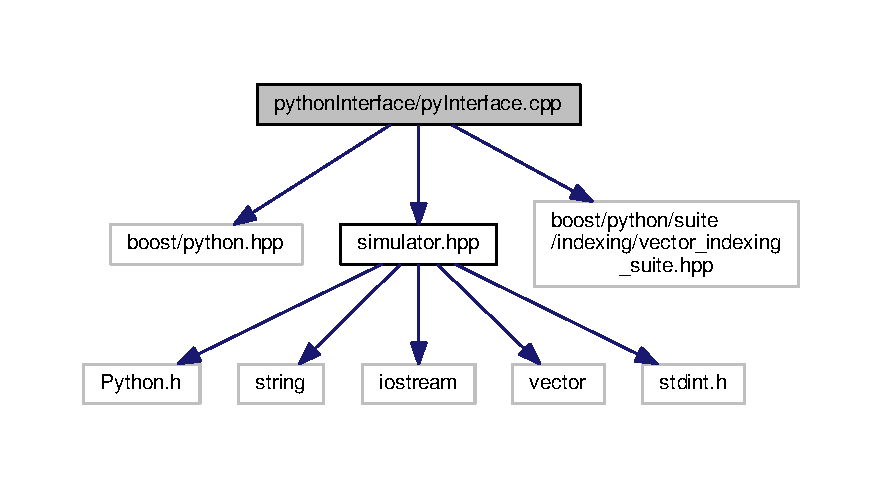
\includegraphics[width=350pt]{py_interface_8cpp__incl}
\end{center}
\end{figure}
\subsection*{Typedefs}
\begin{DoxyCompactItemize}
\item 
using \hyperlink{py_interface_8cpp_ac01dafe2b6cd1153cac94bbd66bec55d}{M\-E\-M\-\_\-type} = vector$<$ uint16\-\_\-t $>$
\end{DoxyCompactItemize}
\subsection*{Functions}
\begin{DoxyCompactItemize}
\item 
\hyperlink{py_interface_8cpp_a0801f9b19524358e13091323fb8929e2}{B\-O\-O\-S\-T\-\_\-\-P\-Y\-T\-H\-O\-N\-\_\-\-M\-O\-D\-U\-L\-E} (pylc3)
\end{DoxyCompactItemize}


\subsection{Typedef Documentation}
\hypertarget{py_interface_8cpp_ac01dafe2b6cd1153cac94bbd66bec55d}{\index{py\-Interface.\-cpp@{py\-Interface.\-cpp}!M\-E\-M\-\_\-type@{M\-E\-M\-\_\-type}}
\index{M\-E\-M\-\_\-type@{M\-E\-M\-\_\-type}!pyInterface.cpp@{py\-Interface.\-cpp}}
\subsubsection[{M\-E\-M\-\_\-type}]{\setlength{\rightskip}{0pt plus 5cm}using {\bf M\-E\-M\-\_\-type} =  vector$<$uint16\-\_\-t$>$}}\label{py_interface_8cpp_ac01dafe2b6cd1153cac94bbd66bec55d}


Definition at line 6 of file py\-Interface.\-cpp.



\subsection{Function Documentation}
\hypertarget{py_interface_8cpp_a0801f9b19524358e13091323fb8929e2}{\index{py\-Interface.\-cpp@{py\-Interface.\-cpp}!B\-O\-O\-S\-T\-\_\-\-P\-Y\-T\-H\-O\-N\-\_\-\-M\-O\-D\-U\-L\-E@{B\-O\-O\-S\-T\-\_\-\-P\-Y\-T\-H\-O\-N\-\_\-\-M\-O\-D\-U\-L\-E}}
\index{B\-O\-O\-S\-T\-\_\-\-P\-Y\-T\-H\-O\-N\-\_\-\-M\-O\-D\-U\-L\-E@{B\-O\-O\-S\-T\-\_\-\-P\-Y\-T\-H\-O\-N\-\_\-\-M\-O\-D\-U\-L\-E}!pyInterface.cpp@{py\-Interface.\-cpp}}
\subsubsection[{B\-O\-O\-S\-T\-\_\-\-P\-Y\-T\-H\-O\-N\-\_\-\-M\-O\-D\-U\-L\-E}]{\setlength{\rightskip}{0pt plus 5cm}B\-O\-O\-S\-T\-\_\-\-P\-Y\-T\-H\-O\-N\-\_\-\-M\-O\-D\-U\-L\-E (
\begin{DoxyParamCaption}
\item[{pylc3}]{}
\end{DoxyParamCaption}
)}}\label{py_interface_8cpp_a0801f9b19524358e13091323fb8929e2}


Definition at line 9 of file py\-Interface.\-cpp.



Here is the call graph for this function\-:
\nopagebreak
\begin{figure}[H]
\begin{center}
\leavevmode
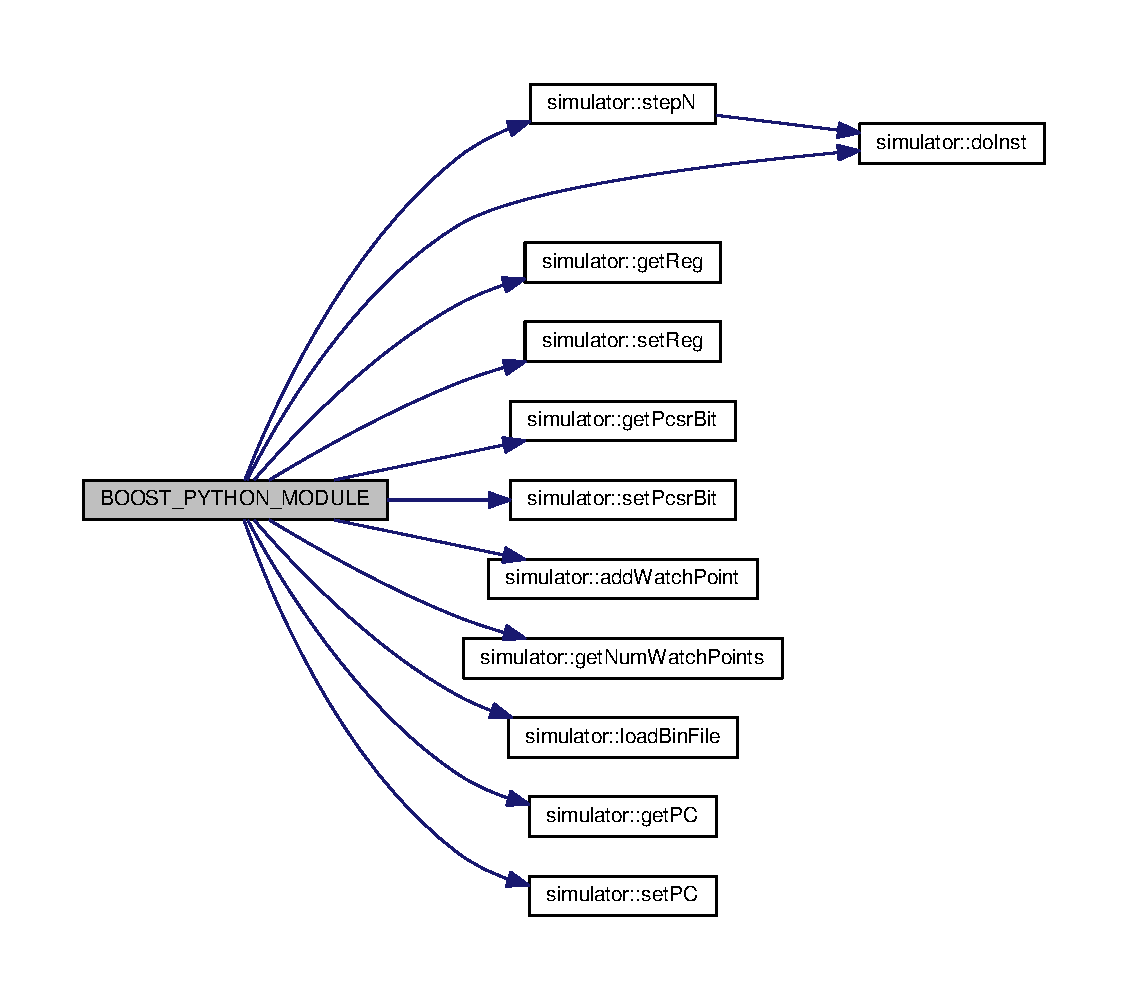
\includegraphics[width=350pt]{py_interface_8cpp_a0801f9b19524358e13091323fb8929e2_cgraph}
\end{center}
\end{figure}



\hypertarget{py_interface_8d}{\section{python\-Interface/py\-Interface.d File Reference}
\label{py_interface_8d}\index{python\-Interface/py\-Interface.\-d@{python\-Interface/py\-Interface.\-d}}
}

\hypertarget{_r_e_a_d_m_e_8md}{\section{R\-E\-A\-D\-M\-E.\-md File Reference}
\label{_r_e_a_d_m_e_8md}\index{R\-E\-A\-D\-M\-E.\-md@{R\-E\-A\-D\-M\-E.\-md}}
}

\hypertarget{simulator-internals_8hpp}{\section{simulator-\/internals.hpp File Reference}
\label{simulator-internals_8hpp}\index{simulator-\/internals.\-hpp@{simulator-\/internals.\-hpp}}
}
This graph shows which files directly or indirectly include this file\-:
\nopagebreak
\begin{figure}[H]
\begin{center}
\leavevmode
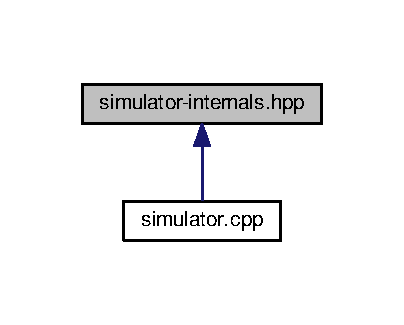
\includegraphics[width=194pt]{simulator-internals_8hpp__dep__incl}
\end{center}
\end{figure}
\subsection*{Enumerations}
\begin{DoxyCompactItemize}
\item 
enum \hyperlink{simulator-internals_8hpp_a299fc707c775371e0b2b0495ccb6158e}{opcode} \{ \\*
\hyperlink{simulator-internals_8hpp_a299fc707c775371e0b2b0495ccb6158ea60a57eed407e7df8eb3bf49f61a042c1}{B\-R} = 0, 
\hyperlink{simulator-internals_8hpp_a299fc707c775371e0b2b0495ccb6158eacfcf145f2788bf340ff3f3098bc54909}{A\-D\-D} = 1, 
\hyperlink{simulator-internals_8hpp_a299fc707c775371e0b2b0495ccb6158ea24a5a956f8abcaacbde751c49c7d5001}{L\-D} = 2, 
\hyperlink{simulator-internals_8hpp_a299fc707c775371e0b2b0495ccb6158ea200bf26d1a70596904b82da10880c2f1}{S\-T} = 3, 
\\*
\hyperlink{simulator-internals_8hpp_a299fc707c775371e0b2b0495ccb6158eafff003cfe0101900ba74af943d311b85}{J\-S\-R} = 4, 
\hyperlink{simulator-internals_8hpp_a299fc707c775371e0b2b0495ccb6158ea865555c9f2e0458a7078486aa1b3254f}{A\-N\-D} = 5, 
\hyperlink{simulator-internals_8hpp_a299fc707c775371e0b2b0495ccb6158ea3e095ea6639ee2dec5fbaedf0ff59753}{L\-D\-R} = 6, 
\hyperlink{simulator-internals_8hpp_a299fc707c775371e0b2b0495ccb6158eaec41e801b43cfbec49d343c900360bf9}{S\-T\-R} = 7, 
\\*
\hyperlink{simulator-internals_8hpp_a299fc707c775371e0b2b0495ccb6158ea06d724c2825230cf5893f6985bf6f4bd}{R\-T\-I} = 8, 
\hyperlink{simulator-internals_8hpp_a299fc707c775371e0b2b0495ccb6158ea0378ebc895849163b249d0b330257dd6}{N\-O\-T} = 9, 
\hyperlink{simulator-internals_8hpp_a299fc707c775371e0b2b0495ccb6158ea98ab2bcdb68b0eac90c7e4ae2fbac19d}{L\-D\-I} = 10, 
\hyperlink{simulator-internals_8hpp_a299fc707c775371e0b2b0495ccb6158eacca7effd335d03e4f287f85ae0a73542}{S\-T\-I} = 11, 
\\*
\hyperlink{simulator-internals_8hpp_a299fc707c775371e0b2b0495ccb6158ea227d95ecea3ff1219ddb58bb03d17d5a}{J\-M\-P} = 12, 
\hyperlink{simulator-internals_8hpp_a299fc707c775371e0b2b0495ccb6158eafe4c21755babfece7188666f75c7386b}{R\-E\-S\-E\-R\-V\-E\-D} = 13, 
\hyperlink{simulator-internals_8hpp_a299fc707c775371e0b2b0495ccb6158ea42c948acd2badbe13a2ff7c4484ffc05}{L\-E\-A} = 14, 
\hyperlink{simulator-internals_8hpp_a299fc707c775371e0b2b0495ccb6158eac0533b6cb94383273589b6764c8a0796}{T\-R\-A\-P} = 15
 \}
\end{DoxyCompactItemize}


\subsection{Enumeration Type Documentation}
\hypertarget{simulator-internals_8hpp_a299fc707c775371e0b2b0495ccb6158e}{\index{simulator-\/internals.\-hpp@{simulator-\/internals.\-hpp}!opcode@{opcode}}
\index{opcode@{opcode}!simulator-internals.hpp@{simulator-\/internals.\-hpp}}
\subsubsection[{opcode}]{\setlength{\rightskip}{0pt plus 5cm}enum {\bf opcode}}}\label{simulator-internals_8hpp_a299fc707c775371e0b2b0495ccb6158e}
\begin{Desc}
\item[Enumerator]\par
\begin{description}
\index{B\-R@{B\-R}!simulator-\/internals.\-hpp@{simulator-\/internals.\-hpp}}\index{simulator-\/internals.\-hpp@{simulator-\/internals.\-hpp}!B\-R@{B\-R}}\item[{\em 
\hypertarget{simulator-internals_8hpp_a299fc707c775371e0b2b0495ccb6158ea60a57eed407e7df8eb3bf49f61a042c1}{B\-R}\label{simulator-internals_8hpp_a299fc707c775371e0b2b0495ccb6158ea60a57eed407e7df8eb3bf49f61a042c1}
}]\index{A\-D\-D@{A\-D\-D}!simulator-\/internals.\-hpp@{simulator-\/internals.\-hpp}}\index{simulator-\/internals.\-hpp@{simulator-\/internals.\-hpp}!A\-D\-D@{A\-D\-D}}\item[{\em 
\hypertarget{simulator-internals_8hpp_a299fc707c775371e0b2b0495ccb6158eacfcf145f2788bf340ff3f3098bc54909}{A\-D\-D}\label{simulator-internals_8hpp_a299fc707c775371e0b2b0495ccb6158eacfcf145f2788bf340ff3f3098bc54909}
}]\index{L\-D@{L\-D}!simulator-\/internals.\-hpp@{simulator-\/internals.\-hpp}}\index{simulator-\/internals.\-hpp@{simulator-\/internals.\-hpp}!L\-D@{L\-D}}\item[{\em 
\hypertarget{simulator-internals_8hpp_a299fc707c775371e0b2b0495ccb6158ea24a5a956f8abcaacbde751c49c7d5001}{L\-D}\label{simulator-internals_8hpp_a299fc707c775371e0b2b0495ccb6158ea24a5a956f8abcaacbde751c49c7d5001}
}]\index{S\-T@{S\-T}!simulator-\/internals.\-hpp@{simulator-\/internals.\-hpp}}\index{simulator-\/internals.\-hpp@{simulator-\/internals.\-hpp}!S\-T@{S\-T}}\item[{\em 
\hypertarget{simulator-internals_8hpp_a299fc707c775371e0b2b0495ccb6158ea200bf26d1a70596904b82da10880c2f1}{S\-T}\label{simulator-internals_8hpp_a299fc707c775371e0b2b0495ccb6158ea200bf26d1a70596904b82da10880c2f1}
}]\index{J\-S\-R@{J\-S\-R}!simulator-\/internals.\-hpp@{simulator-\/internals.\-hpp}}\index{simulator-\/internals.\-hpp@{simulator-\/internals.\-hpp}!J\-S\-R@{J\-S\-R}}\item[{\em 
\hypertarget{simulator-internals_8hpp_a299fc707c775371e0b2b0495ccb6158eafff003cfe0101900ba74af943d311b85}{J\-S\-R}\label{simulator-internals_8hpp_a299fc707c775371e0b2b0495ccb6158eafff003cfe0101900ba74af943d311b85}
}]\index{A\-N\-D@{A\-N\-D}!simulator-\/internals.\-hpp@{simulator-\/internals.\-hpp}}\index{simulator-\/internals.\-hpp@{simulator-\/internals.\-hpp}!A\-N\-D@{A\-N\-D}}\item[{\em 
\hypertarget{simulator-internals_8hpp_a299fc707c775371e0b2b0495ccb6158ea865555c9f2e0458a7078486aa1b3254f}{A\-N\-D}\label{simulator-internals_8hpp_a299fc707c775371e0b2b0495ccb6158ea865555c9f2e0458a7078486aa1b3254f}
}]\index{L\-D\-R@{L\-D\-R}!simulator-\/internals.\-hpp@{simulator-\/internals.\-hpp}}\index{simulator-\/internals.\-hpp@{simulator-\/internals.\-hpp}!L\-D\-R@{L\-D\-R}}\item[{\em 
\hypertarget{simulator-internals_8hpp_a299fc707c775371e0b2b0495ccb6158ea3e095ea6639ee2dec5fbaedf0ff59753}{L\-D\-R}\label{simulator-internals_8hpp_a299fc707c775371e0b2b0495ccb6158ea3e095ea6639ee2dec5fbaedf0ff59753}
}]\index{S\-T\-R@{S\-T\-R}!simulator-\/internals.\-hpp@{simulator-\/internals.\-hpp}}\index{simulator-\/internals.\-hpp@{simulator-\/internals.\-hpp}!S\-T\-R@{S\-T\-R}}\item[{\em 
\hypertarget{simulator-internals_8hpp_a299fc707c775371e0b2b0495ccb6158eaec41e801b43cfbec49d343c900360bf9}{S\-T\-R}\label{simulator-internals_8hpp_a299fc707c775371e0b2b0495ccb6158eaec41e801b43cfbec49d343c900360bf9}
}]\index{R\-T\-I@{R\-T\-I}!simulator-\/internals.\-hpp@{simulator-\/internals.\-hpp}}\index{simulator-\/internals.\-hpp@{simulator-\/internals.\-hpp}!R\-T\-I@{R\-T\-I}}\item[{\em 
\hypertarget{simulator-internals_8hpp_a299fc707c775371e0b2b0495ccb6158ea06d724c2825230cf5893f6985bf6f4bd}{R\-T\-I}\label{simulator-internals_8hpp_a299fc707c775371e0b2b0495ccb6158ea06d724c2825230cf5893f6985bf6f4bd}
}]\index{N\-O\-T@{N\-O\-T}!simulator-\/internals.\-hpp@{simulator-\/internals.\-hpp}}\index{simulator-\/internals.\-hpp@{simulator-\/internals.\-hpp}!N\-O\-T@{N\-O\-T}}\item[{\em 
\hypertarget{simulator-internals_8hpp_a299fc707c775371e0b2b0495ccb6158ea0378ebc895849163b249d0b330257dd6}{N\-O\-T}\label{simulator-internals_8hpp_a299fc707c775371e0b2b0495ccb6158ea0378ebc895849163b249d0b330257dd6}
}]\index{L\-D\-I@{L\-D\-I}!simulator-\/internals.\-hpp@{simulator-\/internals.\-hpp}}\index{simulator-\/internals.\-hpp@{simulator-\/internals.\-hpp}!L\-D\-I@{L\-D\-I}}\item[{\em 
\hypertarget{simulator-internals_8hpp_a299fc707c775371e0b2b0495ccb6158ea98ab2bcdb68b0eac90c7e4ae2fbac19d}{L\-D\-I}\label{simulator-internals_8hpp_a299fc707c775371e0b2b0495ccb6158ea98ab2bcdb68b0eac90c7e4ae2fbac19d}
}]\index{S\-T\-I@{S\-T\-I}!simulator-\/internals.\-hpp@{simulator-\/internals.\-hpp}}\index{simulator-\/internals.\-hpp@{simulator-\/internals.\-hpp}!S\-T\-I@{S\-T\-I}}\item[{\em 
\hypertarget{simulator-internals_8hpp_a299fc707c775371e0b2b0495ccb6158eacca7effd335d03e4f287f85ae0a73542}{S\-T\-I}\label{simulator-internals_8hpp_a299fc707c775371e0b2b0495ccb6158eacca7effd335d03e4f287f85ae0a73542}
}]\index{J\-M\-P@{J\-M\-P}!simulator-\/internals.\-hpp@{simulator-\/internals.\-hpp}}\index{simulator-\/internals.\-hpp@{simulator-\/internals.\-hpp}!J\-M\-P@{J\-M\-P}}\item[{\em 
\hypertarget{simulator-internals_8hpp_a299fc707c775371e0b2b0495ccb6158ea227d95ecea3ff1219ddb58bb03d17d5a}{J\-M\-P}\label{simulator-internals_8hpp_a299fc707c775371e0b2b0495ccb6158ea227d95ecea3ff1219ddb58bb03d17d5a}
}]\index{R\-E\-S\-E\-R\-V\-E\-D@{R\-E\-S\-E\-R\-V\-E\-D}!simulator-\/internals.\-hpp@{simulator-\/internals.\-hpp}}\index{simulator-\/internals.\-hpp@{simulator-\/internals.\-hpp}!R\-E\-S\-E\-R\-V\-E\-D@{R\-E\-S\-E\-R\-V\-E\-D}}\item[{\em 
\hypertarget{simulator-internals_8hpp_a299fc707c775371e0b2b0495ccb6158eafe4c21755babfece7188666f75c7386b}{R\-E\-S\-E\-R\-V\-E\-D}\label{simulator-internals_8hpp_a299fc707c775371e0b2b0495ccb6158eafe4c21755babfece7188666f75c7386b}
}]\index{L\-E\-A@{L\-E\-A}!simulator-\/internals.\-hpp@{simulator-\/internals.\-hpp}}\index{simulator-\/internals.\-hpp@{simulator-\/internals.\-hpp}!L\-E\-A@{L\-E\-A}}\item[{\em 
\hypertarget{simulator-internals_8hpp_a299fc707c775371e0b2b0495ccb6158ea42c948acd2badbe13a2ff7c4484ffc05}{L\-E\-A}\label{simulator-internals_8hpp_a299fc707c775371e0b2b0495ccb6158ea42c948acd2badbe13a2ff7c4484ffc05}
}]\index{T\-R\-A\-P@{T\-R\-A\-P}!simulator-\/internals.\-hpp@{simulator-\/internals.\-hpp}}\index{simulator-\/internals.\-hpp@{simulator-\/internals.\-hpp}!T\-R\-A\-P@{T\-R\-A\-P}}\item[{\em 
\hypertarget{simulator-internals_8hpp_a299fc707c775371e0b2b0495ccb6158eac0533b6cb94383273589b6764c8a0796}{T\-R\-A\-P}\label{simulator-internals_8hpp_a299fc707c775371e0b2b0495ccb6158eac0533b6cb94383273589b6764c8a0796}
}]\end{description}
\end{Desc}


Definition at line 3 of file simulator-\/internals.\-hpp.


\hypertarget{simulator_8cpp}{\section{simulator.\-cpp File Reference}
\label{simulator_8cpp}\index{simulator.\-cpp@{simulator.\-cpp}}
}
{\ttfamily \#include \char`\"{}simulator.\-hpp\char`\"{}}\\*
{\ttfamily \#include \char`\"{}simulator-\/internals.\-hpp\char`\"{}}\\*
{\ttfamily \#include $<$boost/python.\-hpp$>$}\\*
{\ttfamily \#include $<$fstream$>$}\\*
Include dependency graph for simulator.\-cpp\-:
\nopagebreak
\begin{figure}[H]
\begin{center}
\leavevmode
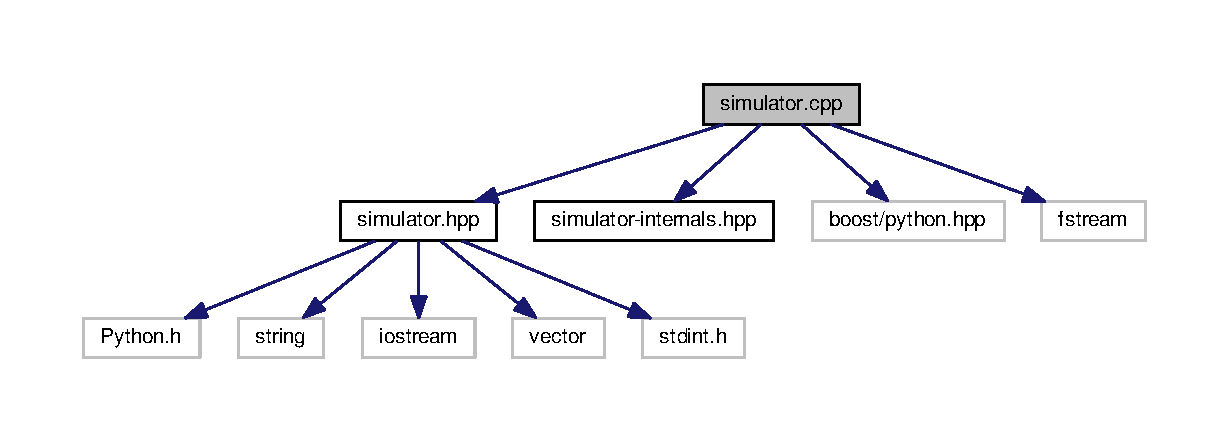
\includegraphics[width=350pt]{simulator_8cpp__incl}
\end{center}
\end{figure}
\subsection*{Functions}
\begin{DoxyCompactItemize}
\item 
void \hyperlink{simulator_8cpp_a8bff8d845e676b34b784598ab73a96b8}{call\-Callback} (struct \hyperlink{struct_watch_point}{Watch\-Point} to\-Call)
\begin{DoxyCompactList}\small\item\em call watchpoint callbacks \end{DoxyCompactList}\end{DoxyCompactItemize}


\subsection{Function Documentation}
\hypertarget{simulator_8cpp_a8bff8d845e676b34b784598ab73a96b8}{\index{simulator.\-cpp@{simulator.\-cpp}!call\-Callback@{call\-Callback}}
\index{call\-Callback@{call\-Callback}!simulator.cpp@{simulator.\-cpp}}
\subsubsection[{call\-Callback}]{\setlength{\rightskip}{0pt plus 5cm}void call\-Callback (
\begin{DoxyParamCaption}
\item[{struct {\bf Watch\-Point}}]{to\-Call}
\end{DoxyParamCaption}
)}}\label{simulator_8cpp_a8bff8d845e676b34b784598ab73a96b8}


call watchpoint callbacks 

Watchpoints have python callbacks, e.\-g. a print function or some other process. Equivelent to on\-Changed(mem\mbox{[}\-Address\mbox{]}) do callback


\begin{DoxyParams}{Parameters}
{\em \hyperlink{struct_watch_point}{Watch\-Point}} & Triggered watch point \\
\hline
\end{DoxyParams}


Definition at line 64 of file simulator.\-cpp.


\hypertarget{simulator_8d}{\section{simulator.\-d File Reference}
\label{simulator_8d}\index{simulator.\-d@{simulator.\-d}}
}

\hypertarget{simulator_8hpp}{\section{simulator.\-hpp File Reference}
\label{simulator_8hpp}\index{simulator.\-hpp@{simulator.\-hpp}}
}
{\ttfamily \#include $<$Python.\-h$>$}\\*
{\ttfamily \#include $<$string$>$}\\*
{\ttfamily \#include $<$iostream$>$}\\*
{\ttfamily \#include $<$vector$>$}\\*
{\ttfamily \#include $<$stdint.\-h$>$}\\*
Include dependency graph for simulator.\-hpp\-:
\nopagebreak
\begin{figure}[H]
\begin{center}
\leavevmode
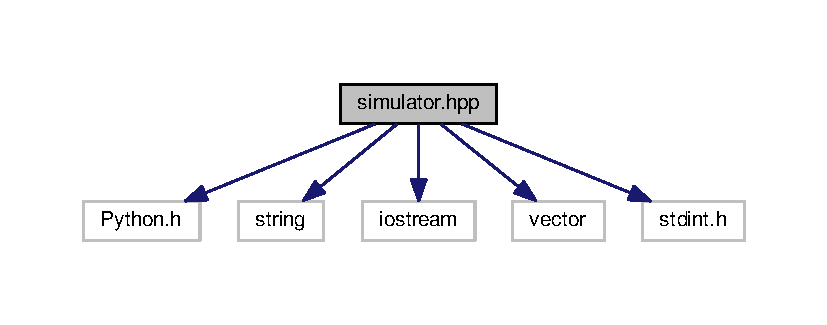
\includegraphics[width=350pt]{simulator_8hpp__incl}
\end{center}
\end{figure}
This graph shows which files directly or indirectly include this file\-:
\nopagebreak
\begin{figure}[H]
\begin{center}
\leavevmode
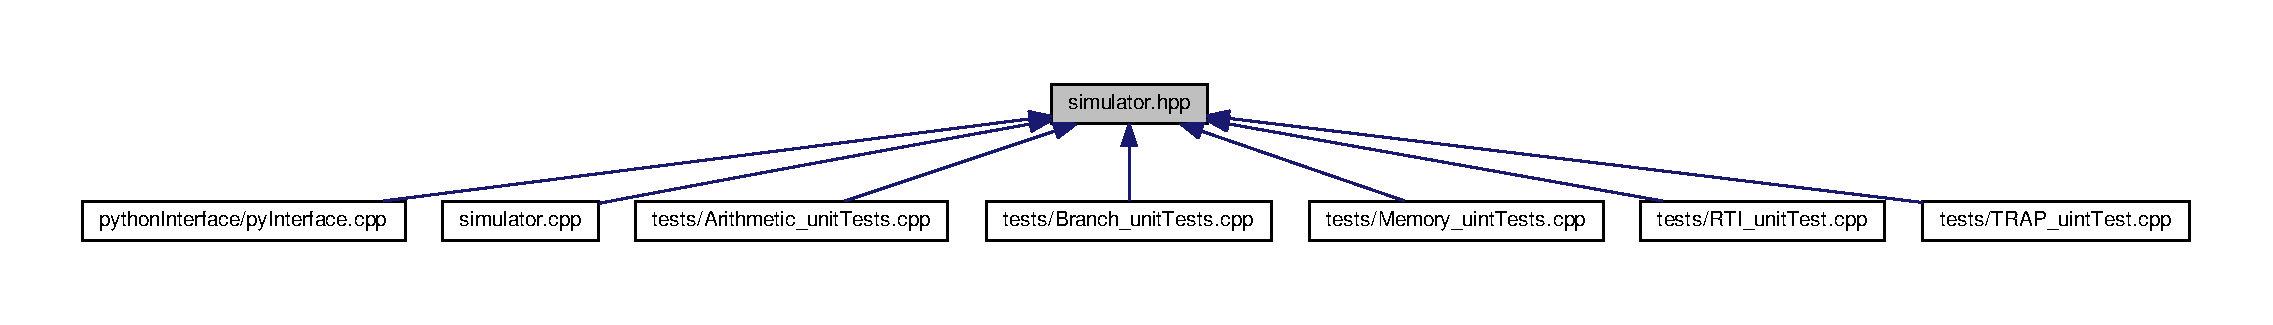
\includegraphics[width=350pt]{simulator_8hpp__dep__incl}
\end{center}
\end{figure}
\subsection*{Classes}
\begin{DoxyCompactItemize}
\item 
struct \hyperlink{struct_watch_point}{Watch\-Point}
\item 
class \hyperlink{classsimulator}{simulator}
\begin{DoxyCompactList}\small\item\em Basic L\-C3 Simulator Class. \end{DoxyCompactList}\end{DoxyCompactItemize}
\subsection*{Variables}
\begin{DoxyCompactItemize}
\item 
constexpr int \hyperlink{simulator_8hpp_aeacd5eb3350ee895e5e2f56398f1055c}{A\-D\-D\-R\-E\-S\-S\-\_\-\-S\-P\-A\-C\-E} = 1$<$$<$16
\item 
constexpr int \hyperlink{simulator_8hpp_a4b883e7c08a7c03b3d36cd5ca84d8ef3}{N\-U\-M\-\_\-\-R\-E\-G\-S} = 8
\end{DoxyCompactItemize}


\subsection{Variable Documentation}
\hypertarget{simulator_8hpp_aeacd5eb3350ee895e5e2f56398f1055c}{\index{simulator.\-hpp@{simulator.\-hpp}!A\-D\-D\-R\-E\-S\-S\-\_\-\-S\-P\-A\-C\-E@{A\-D\-D\-R\-E\-S\-S\-\_\-\-S\-P\-A\-C\-E}}
\index{A\-D\-D\-R\-E\-S\-S\-\_\-\-S\-P\-A\-C\-E@{A\-D\-D\-R\-E\-S\-S\-\_\-\-S\-P\-A\-C\-E}!simulator.hpp@{simulator.\-hpp}}
\subsubsection[{A\-D\-D\-R\-E\-S\-S\-\_\-\-S\-P\-A\-C\-E}]{\setlength{\rightskip}{0pt plus 5cm}constexpr int A\-D\-D\-R\-E\-S\-S\-\_\-\-S\-P\-A\-C\-E = 1$<$$<$16}}\label{simulator_8hpp_aeacd5eb3350ee895e5e2f56398f1055c}


Definition at line 9 of file simulator.\-hpp.

\hypertarget{simulator_8hpp_a4b883e7c08a7c03b3d36cd5ca84d8ef3}{\index{simulator.\-hpp@{simulator.\-hpp}!N\-U\-M\-\_\-\-R\-E\-G\-S@{N\-U\-M\-\_\-\-R\-E\-G\-S}}
\index{N\-U\-M\-\_\-\-R\-E\-G\-S@{N\-U\-M\-\_\-\-R\-E\-G\-S}!simulator.hpp@{simulator.\-hpp}}
\subsubsection[{N\-U\-M\-\_\-\-R\-E\-G\-S}]{\setlength{\rightskip}{0pt plus 5cm}constexpr int N\-U\-M\-\_\-\-R\-E\-G\-S = 8}}\label{simulator_8hpp_a4b883e7c08a7c03b3d36cd5ca84d8ef3}


Definition at line 10 of file simulator.\-hpp.


\hypertarget{simulator_unit_tests_8py}{\section{simulator\-Unit\-Tests.\-py File Reference}
\label{simulator_unit_tests_8py}\index{simulator\-Unit\-Tests.\-py@{simulator\-Unit\-Tests.\-py}}
}
\subsection*{Classes}
\begin{DoxyCompactItemize}
\item 
class \hyperlink{class_qt_l_c3_1_1simulator_unit_tests_1_1_test_add}{Qt\-L\-C3.\-simulator\-Unit\-Tests.\-Test\-Add}
\item 
class \hyperlink{class_qt_l_c3_1_1simulator_unit_tests_1_1_test_and}{Qt\-L\-C3.\-simulator\-Unit\-Tests.\-Test\-And}
\item 
class \hyperlink{class_qt_l_c3_1_1simulator_unit_tests_1_1_test_watch_point}{Qt\-L\-C3.\-simulator\-Unit\-Tests.\-Test\-Watch\-Point}
\end{DoxyCompactItemize}
\subsection*{Namespaces}
\begin{DoxyCompactItemize}
\item 
\hyperlink{namespace_qt_l_c3_1_1simulator_unit_tests}{Qt\-L\-C3.\-simulator\-Unit\-Tests}
\end{DoxyCompactItemize}
\subsection*{Functions}
\begin{DoxyCompactItemize}
\item 
def \hyperlink{namespace_qt_l_c3_1_1simulator_unit_tests_a2d038a14c4230b686d46e0e427e8941e}{Qt\-L\-C3.\-simulator\-Unit\-Tests.\-do\-Test}
\end{DoxyCompactItemize}
\subsection*{Variables}
\begin{DoxyCompactItemize}
\item 
\hyperlink{namespace_qt_l_c3_1_1simulator_unit_tests_a762ffb74f9f8e380299cd1c525932310}{Qt\-L\-C3.\-simulator\-Unit\-Tests.\-false} = False
\item 
\hyperlink{namespace_qt_l_c3_1_1simulator_unit_tests_ac23f444832b767cf808b54d5d6f4bd72}{Qt\-L\-C3.\-simulator\-Unit\-Tests.\-true} = True
\end{DoxyCompactItemize}

\hypertarget{_arithmetic__unit_tests_8cpp}{\section{tests/\-Arithmetic\-\_\-unit\-Tests.cpp File Reference}
\label{_arithmetic__unit_tests_8cpp}\index{tests/\-Arithmetic\-\_\-unit\-Tests.\-cpp@{tests/\-Arithmetic\-\_\-unit\-Tests.\-cpp}}
}
{\ttfamily \#include \char`\"{}simulator.\-hpp\char`\"{}}\\*
{\ttfamily \#include $<$chrono$>$}\\*
{\ttfamily \#include $<$complex$>$}\\*
{\ttfamily \#include $<$cstdint$>$}\\*
{\ttfamily \#include $<$future$>$}\\*
{\ttfamily \#include $<$iostream$>$}\\*
{\ttfamily \#include $<$stdexcept$>$}\\*
{\ttfamily \#include $<$stdint.\-h$>$}\\*
{\ttfamily \#include \char`\"{}gtest/gtest.\-h\char`\"{}}\\*
{\ttfamily \#include \char`\"{}L\-C3\-Helper.\-h\char`\"{}}\\*
Include dependency graph for Arithmetic\-\_\-unit\-Tests.\-cpp\-:
\nopagebreak
\begin{figure}[H]
\begin{center}
\leavevmode
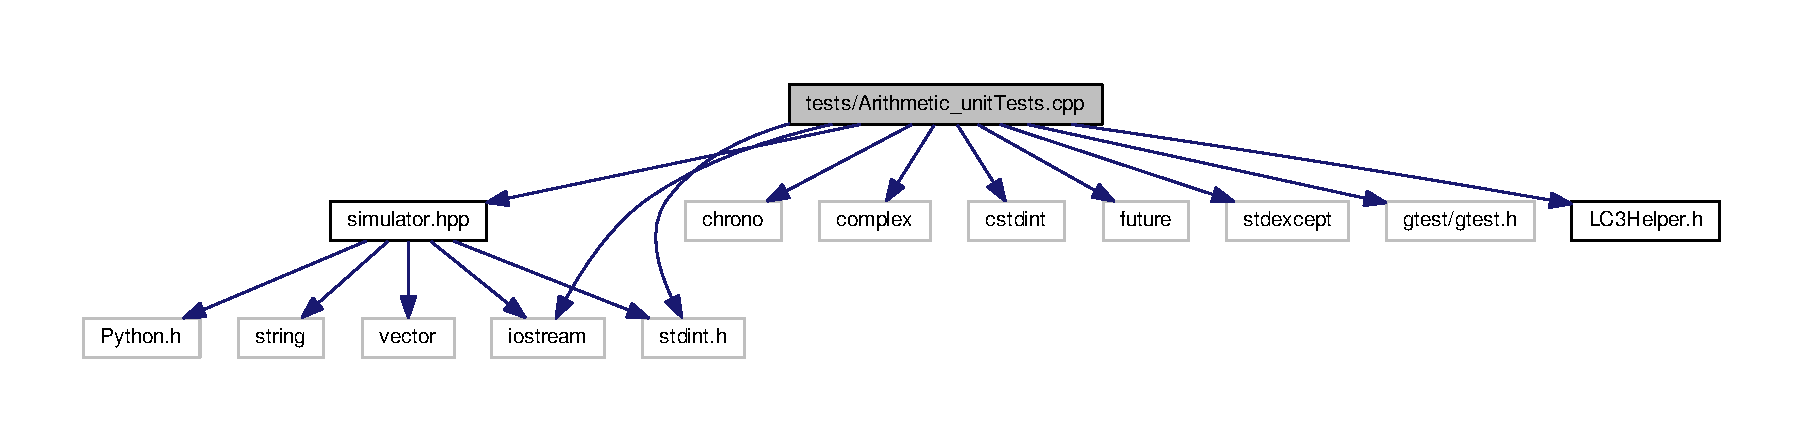
\includegraphics[width=350pt]{_arithmetic__unit_tests_8cpp__incl}
\end{center}
\end{figure}
\subsection*{Functions}
\begin{DoxyCompactItemize}
\item 
\hyperlink{_arithmetic__unit_tests_8cpp_aaf45d748be318d51cc36f6cf34549279}{T\-E\-S\-T} (Check\-A\-D\-D, Register)
\item 
\hyperlink{_arithmetic__unit_tests_8cpp_a9fdad4186bee01e39cb08bf5a3dfee54}{T\-E\-S\-T} (Check\-A\-D\-D, Immediate)
\item 
\hyperlink{_arithmetic__unit_tests_8cpp_a557ff7c04049e9c881e016c0768787c8}{T\-E\-S\-T} (Check\-A\-N\-D, Register)
\item 
\hyperlink{_arithmetic__unit_tests_8cpp_a20d63813c7856e22a3b60296e60e4989}{T\-E\-S\-T} (Check\-A\-N\-D, Immediate)
\item 
\hyperlink{_arithmetic__unit_tests_8cpp_a9d28959b57605460d155aa5b4136a223}{T\-E\-S\-T} (Check\-N\-O\-T, All)
\item 
\hyperlink{_arithmetic__unit_tests_8cpp_a78849b127a51f40aad8639a9a45147af}{T\-E\-S\-T} (Check\-L\-E\-A, Immediate)
\item 
int \hyperlink{_arithmetic__unit_tests_8cpp_a3c04138a5bfe5d72780bb7e82a18e627}{main} (int argc, char $\ast$$\ast$argv)
\end{DoxyCompactItemize}
\subsection*{Variables}
\begin{DoxyCompactItemize}
\item 
\hyperlink{classsimulator}{simulator} \hyperlink{_arithmetic__unit_tests_8cpp_aae71a80982b14fff0075d3d417e2ce4c}{sim}
\end{DoxyCompactItemize}


\subsection{Function Documentation}
\hypertarget{_arithmetic__unit_tests_8cpp_a3c04138a5bfe5d72780bb7e82a18e627}{\index{Arithmetic\-\_\-unit\-Tests.\-cpp@{Arithmetic\-\_\-unit\-Tests.\-cpp}!main@{main}}
\index{main@{main}!Arithmetic_unitTests.cpp@{Arithmetic\-\_\-unit\-Tests.\-cpp}}
\subsubsection[{main}]{\setlength{\rightskip}{0pt plus 5cm}int main (
\begin{DoxyParamCaption}
\item[{int}]{argc, }
\item[{char $\ast$$\ast$}]{argv}
\end{DoxyParamCaption}
)}}\label{_arithmetic__unit_tests_8cpp_a3c04138a5bfe5d72780bb7e82a18e627}


Definition at line 179 of file Arithmetic\-\_\-unit\-Tests.\-cpp.

\hypertarget{_arithmetic__unit_tests_8cpp_aaf45d748be318d51cc36f6cf34549279}{\index{Arithmetic\-\_\-unit\-Tests.\-cpp@{Arithmetic\-\_\-unit\-Tests.\-cpp}!T\-E\-S\-T@{T\-E\-S\-T}}
\index{T\-E\-S\-T@{T\-E\-S\-T}!Arithmetic_unitTests.cpp@{Arithmetic\-\_\-unit\-Tests.\-cpp}}
\subsubsection[{T\-E\-S\-T}]{\setlength{\rightskip}{0pt plus 5cm}T\-E\-S\-T (
\begin{DoxyParamCaption}
\item[{Check\-A\-D\-D}]{, }
\item[{Register}]{}
\end{DoxyParamCaption}
)}}\label{_arithmetic__unit_tests_8cpp_aaf45d748be318d51cc36f6cf34549279}


Definition at line 26 of file Arithmetic\-\_\-unit\-Tests.\-cpp.



Here is the call graph for this function\-:
\nopagebreak
\begin{figure}[H]
\begin{center}
\leavevmode
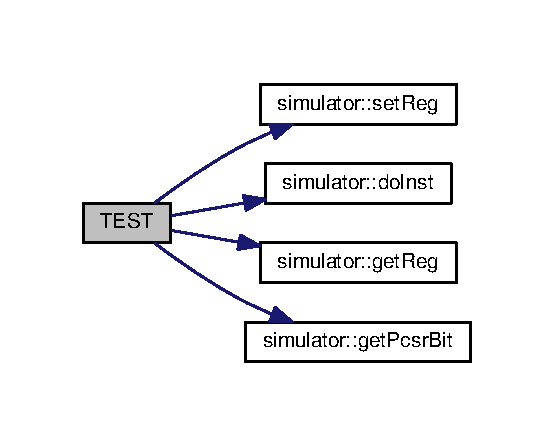
\includegraphics[width=266pt]{_arithmetic__unit_tests_8cpp_aaf45d748be318d51cc36f6cf34549279_cgraph}
\end{center}
\end{figure}


\hypertarget{_arithmetic__unit_tests_8cpp_a9fdad4186bee01e39cb08bf5a3dfee54}{\index{Arithmetic\-\_\-unit\-Tests.\-cpp@{Arithmetic\-\_\-unit\-Tests.\-cpp}!T\-E\-S\-T@{T\-E\-S\-T}}
\index{T\-E\-S\-T@{T\-E\-S\-T}!Arithmetic_unitTests.cpp@{Arithmetic\-\_\-unit\-Tests.\-cpp}}
\subsubsection[{T\-E\-S\-T}]{\setlength{\rightskip}{0pt plus 5cm}T\-E\-S\-T (
\begin{DoxyParamCaption}
\item[{Check\-A\-D\-D}]{, }
\item[{Immediate}]{}
\end{DoxyParamCaption}
)}}\label{_arithmetic__unit_tests_8cpp_a9fdad4186bee01e39cb08bf5a3dfee54}


Definition at line 51 of file Arithmetic\-\_\-unit\-Tests.\-cpp.



Here is the call graph for this function\-:
\nopagebreak
\begin{figure}[H]
\begin{center}
\leavevmode
\includegraphics[width=266pt]{_arithmetic__unit_tests_8cpp_a9fdad4186bee01e39cb08bf5a3dfee54_cgraph}
\end{center}
\end{figure}


\hypertarget{_arithmetic__unit_tests_8cpp_a557ff7c04049e9c881e016c0768787c8}{\index{Arithmetic\-\_\-unit\-Tests.\-cpp@{Arithmetic\-\_\-unit\-Tests.\-cpp}!T\-E\-S\-T@{T\-E\-S\-T}}
\index{T\-E\-S\-T@{T\-E\-S\-T}!Arithmetic_unitTests.cpp@{Arithmetic\-\_\-unit\-Tests.\-cpp}}
\subsubsection[{T\-E\-S\-T}]{\setlength{\rightskip}{0pt plus 5cm}T\-E\-S\-T (
\begin{DoxyParamCaption}
\item[{Check\-A\-N\-D}]{, }
\item[{Register}]{}
\end{DoxyParamCaption}
)}}\label{_arithmetic__unit_tests_8cpp_a557ff7c04049e9c881e016c0768787c8}


Definition at line 74 of file Arithmetic\-\_\-unit\-Tests.\-cpp.



Here is the call graph for this function\-:
\nopagebreak
\begin{figure}[H]
\begin{center}
\leavevmode
\includegraphics[width=266pt]{_arithmetic__unit_tests_8cpp_a557ff7c04049e9c881e016c0768787c8_cgraph}
\end{center}
\end{figure}


\hypertarget{_arithmetic__unit_tests_8cpp_a20d63813c7856e22a3b60296e60e4989}{\index{Arithmetic\-\_\-unit\-Tests.\-cpp@{Arithmetic\-\_\-unit\-Tests.\-cpp}!T\-E\-S\-T@{T\-E\-S\-T}}
\index{T\-E\-S\-T@{T\-E\-S\-T}!Arithmetic_unitTests.cpp@{Arithmetic\-\_\-unit\-Tests.\-cpp}}
\subsubsection[{T\-E\-S\-T}]{\setlength{\rightskip}{0pt plus 5cm}T\-E\-S\-T (
\begin{DoxyParamCaption}
\item[{Check\-A\-N\-D}]{, }
\item[{Immediate}]{}
\end{DoxyParamCaption}
)}}\label{_arithmetic__unit_tests_8cpp_a20d63813c7856e22a3b60296e60e4989}


Definition at line 100 of file Arithmetic\-\_\-unit\-Tests.\-cpp.



Here is the call graph for this function\-:
\nopagebreak
\begin{figure}[H]
\begin{center}
\leavevmode
\includegraphics[width=266pt]{_arithmetic__unit_tests_8cpp_a20d63813c7856e22a3b60296e60e4989_cgraph}
\end{center}
\end{figure}


\hypertarget{_arithmetic__unit_tests_8cpp_a9d28959b57605460d155aa5b4136a223}{\index{Arithmetic\-\_\-unit\-Tests.\-cpp@{Arithmetic\-\_\-unit\-Tests.\-cpp}!T\-E\-S\-T@{T\-E\-S\-T}}
\index{T\-E\-S\-T@{T\-E\-S\-T}!Arithmetic_unitTests.cpp@{Arithmetic\-\_\-unit\-Tests.\-cpp}}
\subsubsection[{T\-E\-S\-T}]{\setlength{\rightskip}{0pt plus 5cm}T\-E\-S\-T (
\begin{DoxyParamCaption}
\item[{Check\-N\-O\-T}]{, }
\item[{All}]{}
\end{DoxyParamCaption}
)}}\label{_arithmetic__unit_tests_8cpp_a9d28959b57605460d155aa5b4136a223}


Definition at line 125 of file Arithmetic\-\_\-unit\-Tests.\-cpp.



Here is the call graph for this function\-:
\nopagebreak
\begin{figure}[H]
\begin{center}
\leavevmode
\includegraphics[width=266pt]{_arithmetic__unit_tests_8cpp_a9d28959b57605460d155aa5b4136a223_cgraph}
\end{center}
\end{figure}


\hypertarget{_arithmetic__unit_tests_8cpp_a78849b127a51f40aad8639a9a45147af}{\index{Arithmetic\-\_\-unit\-Tests.\-cpp@{Arithmetic\-\_\-unit\-Tests.\-cpp}!T\-E\-S\-T@{T\-E\-S\-T}}
\index{T\-E\-S\-T@{T\-E\-S\-T}!Arithmetic_unitTests.cpp@{Arithmetic\-\_\-unit\-Tests.\-cpp}}
\subsubsection[{T\-E\-S\-T}]{\setlength{\rightskip}{0pt plus 5cm}T\-E\-S\-T (
\begin{DoxyParamCaption}
\item[{Check\-L\-E\-A}]{, }
\item[{Immediate}]{}
\end{DoxyParamCaption}
)}}\label{_arithmetic__unit_tests_8cpp_a78849b127a51f40aad8639a9a45147af}


Definition at line 157 of file Arithmetic\-\_\-unit\-Tests.\-cpp.



Here is the call graph for this function\-:
\nopagebreak
\begin{figure}[H]
\begin{center}
\leavevmode
\includegraphics[width=266pt]{_arithmetic__unit_tests_8cpp_a78849b127a51f40aad8639a9a45147af_cgraph}
\end{center}
\end{figure}




\subsection{Variable Documentation}
\hypertarget{_arithmetic__unit_tests_8cpp_aae71a80982b14fff0075d3d417e2ce4c}{\index{Arithmetic\-\_\-unit\-Tests.\-cpp@{Arithmetic\-\_\-unit\-Tests.\-cpp}!sim@{sim}}
\index{sim@{sim}!Arithmetic_unitTests.cpp@{Arithmetic\-\_\-unit\-Tests.\-cpp}}
\subsubsection[{sim}]{\setlength{\rightskip}{0pt plus 5cm}{\bf simulator} sim}}\label{_arithmetic__unit_tests_8cpp_aae71a80982b14fff0075d3d417e2ce4c}


Definition at line 24 of file Arithmetic\-\_\-unit\-Tests.\-cpp.


\hypertarget{_branch__unit_tests_8cpp}{\section{tests/\-Branch\-\_\-unit\-Tests.cpp File Reference}
\label{_branch__unit_tests_8cpp}\index{tests/\-Branch\-\_\-unit\-Tests.\-cpp@{tests/\-Branch\-\_\-unit\-Tests.\-cpp}}
}
{\ttfamily \#include \char`\"{}simulator.\-hpp\char`\"{}}\\*
{\ttfamily \#include $<$chrono$>$}\\*
{\ttfamily \#include $<$complex$>$}\\*
{\ttfamily \#include $<$cstdint$>$}\\*
{\ttfamily \#include $<$future$>$}\\*
{\ttfamily \#include $<$iostream$>$}\\*
{\ttfamily \#include $<$stdexcept$>$}\\*
{\ttfamily \#include $<$stdint.\-h$>$}\\*
{\ttfamily \#include \char`\"{}gtest/gtest.\-h\char`\"{}}\\*
{\ttfamily \#include \char`\"{}L\-C3\-Helper.\-h\char`\"{}}\\*
Include dependency graph for Branch\-\_\-unit\-Tests.\-cpp\-:
\nopagebreak
\begin{figure}[H]
\begin{center}
\leavevmode
\includegraphics[width=350pt]{_branch__unit_tests_8cpp__incl}
\end{center}
\end{figure}
\subsection*{Functions}
\begin{DoxyCompactItemize}
\item 
\hyperlink{_branch__unit_tests_8cpp_a96b918a9269522237fae39a4dc272d80}{T\-E\-S\-T} (Check\-B\-R, All\-Positive)
\item 
\hyperlink{_branch__unit_tests_8cpp_a211341d8479cbee83db7153c81ce7832}{T\-E\-S\-T} (Check\-B\-R, All\-Negative)
\item 
\hyperlink{_branch__unit_tests_8cpp_a4078a4d99ccc0dab38a299fe5516cf2c}{T\-E\-S\-T} (Check\-B\-R, All\-Positive\-Instructions)
\item 
\hyperlink{_branch__unit_tests_8cpp_a85f201d4f74e964c3737e70061f258a9}{T\-E\-S\-T} (Check\-J\-M\-P, All)
\item 
\hyperlink{_branch__unit_tests_8cpp_ae30f008052f85b16f1e1597882024ec3}{T\-E\-S\-T} (Check\-J\-S\-R, All)
\item 
\hyperlink{_branch__unit_tests_8cpp_af93b02668fa6dcd1fedd5cc0256e30da}{T\-E\-S\-T} (Check\-J\-S\-R\-R, All)
\end{DoxyCompactItemize}
\subsection*{Variables}
\begin{DoxyCompactItemize}
\item 
\hyperlink{classsimulator}{simulator} \hyperlink{_branch__unit_tests_8cpp_a82c2ec9c4d1e14b30f656bad1a450ffc}{sim1}
\end{DoxyCompactItemize}


\subsection{Function Documentation}
\hypertarget{_branch__unit_tests_8cpp_a96b918a9269522237fae39a4dc272d80}{\index{Branch\-\_\-unit\-Tests.\-cpp@{Branch\-\_\-unit\-Tests.\-cpp}!T\-E\-S\-T@{T\-E\-S\-T}}
\index{T\-E\-S\-T@{T\-E\-S\-T}!Branch_unitTests.cpp@{Branch\-\_\-unit\-Tests.\-cpp}}
\subsubsection[{T\-E\-S\-T}]{\setlength{\rightskip}{0pt plus 5cm}T\-E\-S\-T (
\begin{DoxyParamCaption}
\item[{Check\-B\-R}]{, }
\item[{All\-Positive}]{}
\end{DoxyParamCaption}
)}}\label{_branch__unit_tests_8cpp_a96b918a9269522237fae39a4dc272d80}


Definition at line 14 of file Branch\-\_\-unit\-Tests.\-cpp.



Here is the call graph for this function\-:
\nopagebreak
\begin{figure}[H]
\begin{center}
\leavevmode
\includegraphics[width=266pt]{_branch__unit_tests_8cpp_a96b918a9269522237fae39a4dc272d80_cgraph}
\end{center}
\end{figure}


\hypertarget{_branch__unit_tests_8cpp_a211341d8479cbee83db7153c81ce7832}{\index{Branch\-\_\-unit\-Tests.\-cpp@{Branch\-\_\-unit\-Tests.\-cpp}!T\-E\-S\-T@{T\-E\-S\-T}}
\index{T\-E\-S\-T@{T\-E\-S\-T}!Branch_unitTests.cpp@{Branch\-\_\-unit\-Tests.\-cpp}}
\subsubsection[{T\-E\-S\-T}]{\setlength{\rightskip}{0pt plus 5cm}T\-E\-S\-T (
\begin{DoxyParamCaption}
\item[{Check\-B\-R}]{, }
\item[{All\-Negative}]{}
\end{DoxyParamCaption}
)}}\label{_branch__unit_tests_8cpp_a211341d8479cbee83db7153c81ce7832}


Definition at line 75 of file Branch\-\_\-unit\-Tests.\-cpp.



Here is the call graph for this function\-:
\nopagebreak
\begin{figure}[H]
\begin{center}
\leavevmode
\includegraphics[width=266pt]{_branch__unit_tests_8cpp_a211341d8479cbee83db7153c81ce7832_cgraph}
\end{center}
\end{figure}


\hypertarget{_branch__unit_tests_8cpp_a4078a4d99ccc0dab38a299fe5516cf2c}{\index{Branch\-\_\-unit\-Tests.\-cpp@{Branch\-\_\-unit\-Tests.\-cpp}!T\-E\-S\-T@{T\-E\-S\-T}}
\index{T\-E\-S\-T@{T\-E\-S\-T}!Branch_unitTests.cpp@{Branch\-\_\-unit\-Tests.\-cpp}}
\subsubsection[{T\-E\-S\-T}]{\setlength{\rightskip}{0pt plus 5cm}T\-E\-S\-T (
\begin{DoxyParamCaption}
\item[{Check\-B\-R}]{, }
\item[{All\-Positive\-Instructions}]{}
\end{DoxyParamCaption}
)}}\label{_branch__unit_tests_8cpp_a4078a4d99ccc0dab38a299fe5516cf2c}


Definition at line 145 of file Branch\-\_\-unit\-Tests.\-cpp.



Here is the call graph for this function\-:
\nopagebreak
\begin{figure}[H]
\begin{center}
\leavevmode
\includegraphics[width=252pt]{_branch__unit_tests_8cpp_a4078a4d99ccc0dab38a299fe5516cf2c_cgraph}
\end{center}
\end{figure}


\hypertarget{_branch__unit_tests_8cpp_a85f201d4f74e964c3737e70061f258a9}{\index{Branch\-\_\-unit\-Tests.\-cpp@{Branch\-\_\-unit\-Tests.\-cpp}!T\-E\-S\-T@{T\-E\-S\-T}}
\index{T\-E\-S\-T@{T\-E\-S\-T}!Branch_unitTests.cpp@{Branch\-\_\-unit\-Tests.\-cpp}}
\subsubsection[{T\-E\-S\-T}]{\setlength{\rightskip}{0pt plus 5cm}T\-E\-S\-T (
\begin{DoxyParamCaption}
\item[{Check\-J\-M\-P}]{, }
\item[{All}]{}
\end{DoxyParamCaption}
)}}\label{_branch__unit_tests_8cpp_a85f201d4f74e964c3737e70061f258a9}


Definition at line 194 of file Branch\-\_\-unit\-Tests.\-cpp.



Here is the call graph for this function\-:
\nopagebreak
\begin{figure}[H]
\begin{center}
\leavevmode
\includegraphics[width=252pt]{_branch__unit_tests_8cpp_a85f201d4f74e964c3737e70061f258a9_cgraph}
\end{center}
\end{figure}


\hypertarget{_branch__unit_tests_8cpp_ae30f008052f85b16f1e1597882024ec3}{\index{Branch\-\_\-unit\-Tests.\-cpp@{Branch\-\_\-unit\-Tests.\-cpp}!T\-E\-S\-T@{T\-E\-S\-T}}
\index{T\-E\-S\-T@{T\-E\-S\-T}!Branch_unitTests.cpp@{Branch\-\_\-unit\-Tests.\-cpp}}
\subsubsection[{T\-E\-S\-T}]{\setlength{\rightskip}{0pt plus 5cm}T\-E\-S\-T (
\begin{DoxyParamCaption}
\item[{Check\-J\-S\-R}]{, }
\item[{All}]{}
\end{DoxyParamCaption}
)}}\label{_branch__unit_tests_8cpp_ae30f008052f85b16f1e1597882024ec3}


Definition at line 221 of file Branch\-\_\-unit\-Tests.\-cpp.



Here is the call graph for this function\-:
\nopagebreak
\begin{figure}[H]
\begin{center}
\leavevmode
\includegraphics[width=252pt]{_branch__unit_tests_8cpp_ae30f008052f85b16f1e1597882024ec3_cgraph}
\end{center}
\end{figure}


\hypertarget{_branch__unit_tests_8cpp_af93b02668fa6dcd1fedd5cc0256e30da}{\index{Branch\-\_\-unit\-Tests.\-cpp@{Branch\-\_\-unit\-Tests.\-cpp}!T\-E\-S\-T@{T\-E\-S\-T}}
\index{T\-E\-S\-T@{T\-E\-S\-T}!Branch_unitTests.cpp@{Branch\-\_\-unit\-Tests.\-cpp}}
\subsubsection[{T\-E\-S\-T}]{\setlength{\rightskip}{0pt plus 5cm}T\-E\-S\-T (
\begin{DoxyParamCaption}
\item[{Check\-J\-S\-R\-R}]{, }
\item[{All}]{}
\end{DoxyParamCaption}
)}}\label{_branch__unit_tests_8cpp_af93b02668fa6dcd1fedd5cc0256e30da}


Definition at line 259 of file Branch\-\_\-unit\-Tests.\-cpp.



Here is the call graph for this function\-:
\nopagebreak
\begin{figure}[H]
\begin{center}
\leavevmode
\includegraphics[width=252pt]{_branch__unit_tests_8cpp_af93b02668fa6dcd1fedd5cc0256e30da_cgraph}
\end{center}
\end{figure}




\subsection{Variable Documentation}
\hypertarget{_branch__unit_tests_8cpp_a82c2ec9c4d1e14b30f656bad1a450ffc}{\index{Branch\-\_\-unit\-Tests.\-cpp@{Branch\-\_\-unit\-Tests.\-cpp}!sim1@{sim1}}
\index{sim1@{sim1}!Branch_unitTests.cpp@{Branch\-\_\-unit\-Tests.\-cpp}}
\subsubsection[{sim1}]{\setlength{\rightskip}{0pt plus 5cm}{\bf simulator} sim1}}\label{_branch__unit_tests_8cpp_a82c2ec9c4d1e14b30f656bad1a450ffc}


Definition at line 12 of file Branch\-\_\-unit\-Tests.\-cpp.


\hypertarget{_l_c3_helper_8h}{\section{tests/\-L\-C3\-Helper.h File Reference}
\label{_l_c3_helper_8h}\index{tests/\-L\-C3\-Helper.\-h@{tests/\-L\-C3\-Helper.\-h}}
}
This graph shows which files directly or indirectly include this file\-:
\nopagebreak
\begin{figure}[H]
\begin{center}
\leavevmode
\includegraphics[width=350pt]{_l_c3_helper_8h__dep__incl}
\end{center}
\end{figure}
\subsection*{Macros}
\begin{DoxyCompactItemize}
\item 
\#define \hyperlink{_l_c3_helper_8h_aa9b849c93cdc3fa4a08a3bc3d09766e6}{S\-E\-T\-D\-R}(x)~(((x) \& 0x7) $<$$<$ 9)
\item 
\#define \hyperlink{_l_c3_helper_8h_a99fd94cbb6f2e44cb7838e498ac75864}{S\-E\-T\-S\-R1}(x)~(((x) \& 0x7) $<$$<$ 6)
\item 
\#define \hyperlink{_l_c3_helper_8h_a021c35ac6036f2af4d4fef5d6a929f4f}{S\-E\-T\-B\-A\-S\-E\-R}(x)~(((x) \& 0x7) $<$$<$ 6)
\item 
\#define \hyperlink{_l_c3_helper_8h_abbb0271e03a9351b45a12e11633848e0}{S\-E\-T\-S\-R2}(x)~(((x) \& 0x7) $<$$<$ 0)
\item 
\#define \hyperlink{_l_c3_helper_8h_aff83afb7cd54a59d11282413dda9b095}{S\-E\-T\-N}(x)~(((x) \& 0x1) $<$$<$ 11)
\item 
\#define \hyperlink{_l_c3_helper_8h_aca7a96d075a20014259b8cddad08ae0b}{S\-E\-T\-Z}(x)~(((x) \& 0x1) $<$$<$ 10)
\item 
\#define \hyperlink{_l_c3_helper_8h_a90022700f86dbec0aa8f7f0b0a6b20e9}{S\-E\-T\-P}(x)~(((x) \& 0x1) $<$$<$ 9)
\item 
\#define \hyperlink{_l_c3_helper_8h_a85572fd40b7cdfec0c3ce8b28651a4b1}{S\-T\-E\-E\-R\-I\-N\-G\-N\-O\-R\-M}~1$<$$<$5
\item 
\#define \hyperlink{_l_c3_helper_8h_ac9f31f726d2933782e2efda7136a25fd}{A\-D\-D\-R}~0x1000
\item 
\#define \hyperlink{_l_c3_helper_8h_a240067f241bac82304fe36d2d4a296da}{A\-D\-D\-I}~\hyperlink{_l_c3_helper_8h_ac9f31f726d2933782e2efda7136a25fd}{A\-D\-D\-R} $\vert$ \hyperlink{_l_c3_helper_8h_a85572fd40b7cdfec0c3ce8b28651a4b1}{S\-T\-E\-E\-R\-I\-N\-G\-N\-O\-R\-M}
\item 
\#define \hyperlink{_l_c3_helper_8h_a850b981e23a59d579d227b208bfbf4a0}{A\-N\-D\-R}~0x5000
\item 
\#define \hyperlink{_l_c3_helper_8h_a6629468bc5e11d36efed350908f2dff4}{A\-N\-D\-I}~\hyperlink{_l_c3_helper_8h_a850b981e23a59d579d227b208bfbf4a0}{A\-N\-D\-R} $\vert$ \hyperlink{_l_c3_helper_8h_a85572fd40b7cdfec0c3ce8b28651a4b1}{S\-T\-E\-E\-R\-I\-N\-G\-N\-O\-R\-M}
\item 
\#define \hyperlink{_l_c3_helper_8h_afa556a68b7c0fcc58cd87c5f36859f30}{B\-R}~0x0000
\item 
\#define \hyperlink{_l_c3_helper_8h_a35e1459a1f52ce4fc0834f47b408ee29}{J\-M\-P}~0x\-C000
\item 
\#define \hyperlink{_l_c3_helper_8h_ae9ef58a66a48face692856868cc1afb7}{J\-S\-R}~0x4800
\item 
\#define \hyperlink{_l_c3_helper_8h_a6df24c255a0cf5049a588354a5f60a7f}{J\-S\-R\-R}~0x4000
\item 
\#define \hyperlink{_l_c3_helper_8h_a9b06fda83ca7a20a56bd6565d6841893}{L\-D}~0x2000
\item 
\#define \hyperlink{_l_c3_helper_8h_a737dc1d07b570f8f87f0fa2bfe11f441}{L\-D\-I}~0x\-A000
\item 
\#define \hyperlink{_l_c3_helper_8h_a9fa6f083fd9b05ac8a6b94f34322661e}{L\-D\-R}~0x6000
\item 
\#define \hyperlink{_l_c3_helper_8h_abba9d672a4e51deeb7ecb7b27f3e4008}{L\-E\-A}~0x\-E000
\item 
\#define \hyperlink{_l_c3_helper_8h_ad3e9fe0ec59d2dbb3982ababa042720c}{N\-O\-T}~0x903\-F
\item 
\#define \hyperlink{_l_c3_helper_8h_ac2544c8b4fe3113b0d6bb62530692c21}{R\-E\-T}~0x\-C1\-C0
\item 
\#define \hyperlink{_l_c3_helper_8h_a16adb4f9e23f6f05317c17678eca62c2}{R\-T\-I}~0x8000
\item 
\#define \hyperlink{_l_c3_helper_8h_ab52cdc475a6866d1be7b5807fb623f50}{S\-T}~0x3000
\item 
\#define \hyperlink{_l_c3_helper_8h_a1171212a040f76ad9630f030efb1653e}{S\-T\-I}~0x\-B000
\item 
\#define \hyperlink{_l_c3_helper_8h_a87f23f9d76e3a2d5658da8dae25f38c4}{S\-T\-R}~0x7000
\item 
\#define \hyperlink{_l_c3_helper_8h_aff974876b14049785960788e714d2a46}{T\-R\-A\-P}~0x\-F000
\item 
\#define \hyperlink{_l_c3_helper_8h_ada695520cf62591eda4972a81edb9b63}{R\-E\-S\-E\-R\-V\-E\-D\-I\-N\-S\-T}~0x\-D000
\end{DoxyCompactItemize}


\subsection{Macro Definition Documentation}
\hypertarget{_l_c3_helper_8h_a240067f241bac82304fe36d2d4a296da}{\index{L\-C3\-Helper.\-h@{L\-C3\-Helper.\-h}!A\-D\-D\-I@{A\-D\-D\-I}}
\index{A\-D\-D\-I@{A\-D\-D\-I}!LC3Helper.h@{L\-C3\-Helper.\-h}}
\subsubsection[{A\-D\-D\-I}]{\setlength{\rightskip}{0pt plus 5cm}\#define A\-D\-D\-I~{\bf A\-D\-D\-R} $\vert$ {\bf S\-T\-E\-E\-R\-I\-N\-G\-N\-O\-R\-M}}}\label{_l_c3_helper_8h_a240067f241bac82304fe36d2d4a296da}


Definition at line 13 of file L\-C3\-Helper.\-h.

\hypertarget{_l_c3_helper_8h_ac9f31f726d2933782e2efda7136a25fd}{\index{L\-C3\-Helper.\-h@{L\-C3\-Helper.\-h}!A\-D\-D\-R@{A\-D\-D\-R}}
\index{A\-D\-D\-R@{A\-D\-D\-R}!LC3Helper.h@{L\-C3\-Helper.\-h}}
\subsubsection[{A\-D\-D\-R}]{\setlength{\rightskip}{0pt plus 5cm}\#define A\-D\-D\-R~0x1000}}\label{_l_c3_helper_8h_ac9f31f726d2933782e2efda7136a25fd}


Definition at line 12 of file L\-C3\-Helper.\-h.

\hypertarget{_l_c3_helper_8h_a6629468bc5e11d36efed350908f2dff4}{\index{L\-C3\-Helper.\-h@{L\-C3\-Helper.\-h}!A\-N\-D\-I@{A\-N\-D\-I}}
\index{A\-N\-D\-I@{A\-N\-D\-I}!LC3Helper.h@{L\-C3\-Helper.\-h}}
\subsubsection[{A\-N\-D\-I}]{\setlength{\rightskip}{0pt plus 5cm}\#define A\-N\-D\-I~{\bf A\-N\-D\-R} $\vert$ {\bf S\-T\-E\-E\-R\-I\-N\-G\-N\-O\-R\-M}}}\label{_l_c3_helper_8h_a6629468bc5e11d36efed350908f2dff4}


Definition at line 15 of file L\-C3\-Helper.\-h.

\hypertarget{_l_c3_helper_8h_a850b981e23a59d579d227b208bfbf4a0}{\index{L\-C3\-Helper.\-h@{L\-C3\-Helper.\-h}!A\-N\-D\-R@{A\-N\-D\-R}}
\index{A\-N\-D\-R@{A\-N\-D\-R}!LC3Helper.h@{L\-C3\-Helper.\-h}}
\subsubsection[{A\-N\-D\-R}]{\setlength{\rightskip}{0pt plus 5cm}\#define A\-N\-D\-R~0x5000}}\label{_l_c3_helper_8h_a850b981e23a59d579d227b208bfbf4a0}


Definition at line 14 of file L\-C3\-Helper.\-h.

\hypertarget{_l_c3_helper_8h_afa556a68b7c0fcc58cd87c5f36859f30}{\index{L\-C3\-Helper.\-h@{L\-C3\-Helper.\-h}!B\-R@{B\-R}}
\index{B\-R@{B\-R}!LC3Helper.h@{L\-C3\-Helper.\-h}}
\subsubsection[{B\-R}]{\setlength{\rightskip}{0pt plus 5cm}\#define B\-R~0x0000}}\label{_l_c3_helper_8h_afa556a68b7c0fcc58cd87c5f36859f30}


Definition at line 16 of file L\-C3\-Helper.\-h.

\hypertarget{_l_c3_helper_8h_a35e1459a1f52ce4fc0834f47b408ee29}{\index{L\-C3\-Helper.\-h@{L\-C3\-Helper.\-h}!J\-M\-P@{J\-M\-P}}
\index{J\-M\-P@{J\-M\-P}!LC3Helper.h@{L\-C3\-Helper.\-h}}
\subsubsection[{J\-M\-P}]{\setlength{\rightskip}{0pt plus 5cm}\#define J\-M\-P~0x\-C000}}\label{_l_c3_helper_8h_a35e1459a1f52ce4fc0834f47b408ee29}


Definition at line 17 of file L\-C3\-Helper.\-h.

\hypertarget{_l_c3_helper_8h_ae9ef58a66a48face692856868cc1afb7}{\index{L\-C3\-Helper.\-h@{L\-C3\-Helper.\-h}!J\-S\-R@{J\-S\-R}}
\index{J\-S\-R@{J\-S\-R}!LC3Helper.h@{L\-C3\-Helper.\-h}}
\subsubsection[{J\-S\-R}]{\setlength{\rightskip}{0pt plus 5cm}\#define J\-S\-R~0x4800}}\label{_l_c3_helper_8h_ae9ef58a66a48face692856868cc1afb7}


Definition at line 18 of file L\-C3\-Helper.\-h.

\hypertarget{_l_c3_helper_8h_a6df24c255a0cf5049a588354a5f60a7f}{\index{L\-C3\-Helper.\-h@{L\-C3\-Helper.\-h}!J\-S\-R\-R@{J\-S\-R\-R}}
\index{J\-S\-R\-R@{J\-S\-R\-R}!LC3Helper.h@{L\-C3\-Helper.\-h}}
\subsubsection[{J\-S\-R\-R}]{\setlength{\rightskip}{0pt plus 5cm}\#define J\-S\-R\-R~0x4000}}\label{_l_c3_helper_8h_a6df24c255a0cf5049a588354a5f60a7f}


Definition at line 19 of file L\-C3\-Helper.\-h.

\hypertarget{_l_c3_helper_8h_a9b06fda83ca7a20a56bd6565d6841893}{\index{L\-C3\-Helper.\-h@{L\-C3\-Helper.\-h}!L\-D@{L\-D}}
\index{L\-D@{L\-D}!LC3Helper.h@{L\-C3\-Helper.\-h}}
\subsubsection[{L\-D}]{\setlength{\rightskip}{0pt plus 5cm}\#define L\-D~0x2000}}\label{_l_c3_helper_8h_a9b06fda83ca7a20a56bd6565d6841893}


Definition at line 20 of file L\-C3\-Helper.\-h.

\hypertarget{_l_c3_helper_8h_a737dc1d07b570f8f87f0fa2bfe11f441}{\index{L\-C3\-Helper.\-h@{L\-C3\-Helper.\-h}!L\-D\-I@{L\-D\-I}}
\index{L\-D\-I@{L\-D\-I}!LC3Helper.h@{L\-C3\-Helper.\-h}}
\subsubsection[{L\-D\-I}]{\setlength{\rightskip}{0pt plus 5cm}\#define L\-D\-I~0x\-A000}}\label{_l_c3_helper_8h_a737dc1d07b570f8f87f0fa2bfe11f441}


Definition at line 21 of file L\-C3\-Helper.\-h.

\hypertarget{_l_c3_helper_8h_a9fa6f083fd9b05ac8a6b94f34322661e}{\index{L\-C3\-Helper.\-h@{L\-C3\-Helper.\-h}!L\-D\-R@{L\-D\-R}}
\index{L\-D\-R@{L\-D\-R}!LC3Helper.h@{L\-C3\-Helper.\-h}}
\subsubsection[{L\-D\-R}]{\setlength{\rightskip}{0pt plus 5cm}\#define L\-D\-R~0x6000}}\label{_l_c3_helper_8h_a9fa6f083fd9b05ac8a6b94f34322661e}


Definition at line 22 of file L\-C3\-Helper.\-h.

\hypertarget{_l_c3_helper_8h_abba9d672a4e51deeb7ecb7b27f3e4008}{\index{L\-C3\-Helper.\-h@{L\-C3\-Helper.\-h}!L\-E\-A@{L\-E\-A}}
\index{L\-E\-A@{L\-E\-A}!LC3Helper.h@{L\-C3\-Helper.\-h}}
\subsubsection[{L\-E\-A}]{\setlength{\rightskip}{0pt plus 5cm}\#define L\-E\-A~0x\-E000}}\label{_l_c3_helper_8h_abba9d672a4e51deeb7ecb7b27f3e4008}


Definition at line 23 of file L\-C3\-Helper.\-h.

\hypertarget{_l_c3_helper_8h_ad3e9fe0ec59d2dbb3982ababa042720c}{\index{L\-C3\-Helper.\-h@{L\-C3\-Helper.\-h}!N\-O\-T@{N\-O\-T}}
\index{N\-O\-T@{N\-O\-T}!LC3Helper.h@{L\-C3\-Helper.\-h}}
\subsubsection[{N\-O\-T}]{\setlength{\rightskip}{0pt plus 5cm}\#define N\-O\-T~0x903\-F}}\label{_l_c3_helper_8h_ad3e9fe0ec59d2dbb3982ababa042720c}


Definition at line 24 of file L\-C3\-Helper.\-h.

\hypertarget{_l_c3_helper_8h_ada695520cf62591eda4972a81edb9b63}{\index{L\-C3\-Helper.\-h@{L\-C3\-Helper.\-h}!R\-E\-S\-E\-R\-V\-E\-D\-I\-N\-S\-T@{R\-E\-S\-E\-R\-V\-E\-D\-I\-N\-S\-T}}
\index{R\-E\-S\-E\-R\-V\-E\-D\-I\-N\-S\-T@{R\-E\-S\-E\-R\-V\-E\-D\-I\-N\-S\-T}!LC3Helper.h@{L\-C3\-Helper.\-h}}
\subsubsection[{R\-E\-S\-E\-R\-V\-E\-D\-I\-N\-S\-T}]{\setlength{\rightskip}{0pt plus 5cm}\#define R\-E\-S\-E\-R\-V\-E\-D\-I\-N\-S\-T~0x\-D000}}\label{_l_c3_helper_8h_ada695520cf62591eda4972a81edb9b63}


Definition at line 31 of file L\-C3\-Helper.\-h.

\hypertarget{_l_c3_helper_8h_ac2544c8b4fe3113b0d6bb62530692c21}{\index{L\-C3\-Helper.\-h@{L\-C3\-Helper.\-h}!R\-E\-T@{R\-E\-T}}
\index{R\-E\-T@{R\-E\-T}!LC3Helper.h@{L\-C3\-Helper.\-h}}
\subsubsection[{R\-E\-T}]{\setlength{\rightskip}{0pt plus 5cm}\#define R\-E\-T~0x\-C1\-C0}}\label{_l_c3_helper_8h_ac2544c8b4fe3113b0d6bb62530692c21}


Definition at line 25 of file L\-C3\-Helper.\-h.

\hypertarget{_l_c3_helper_8h_a16adb4f9e23f6f05317c17678eca62c2}{\index{L\-C3\-Helper.\-h@{L\-C3\-Helper.\-h}!R\-T\-I@{R\-T\-I}}
\index{R\-T\-I@{R\-T\-I}!LC3Helper.h@{L\-C3\-Helper.\-h}}
\subsubsection[{R\-T\-I}]{\setlength{\rightskip}{0pt plus 5cm}\#define R\-T\-I~0x8000}}\label{_l_c3_helper_8h_a16adb4f9e23f6f05317c17678eca62c2}


Definition at line 26 of file L\-C3\-Helper.\-h.

\hypertarget{_l_c3_helper_8h_a021c35ac6036f2af4d4fef5d6a929f4f}{\index{L\-C3\-Helper.\-h@{L\-C3\-Helper.\-h}!S\-E\-T\-B\-A\-S\-E\-R@{S\-E\-T\-B\-A\-S\-E\-R}}
\index{S\-E\-T\-B\-A\-S\-E\-R@{S\-E\-T\-B\-A\-S\-E\-R}!LC3Helper.h@{L\-C3\-Helper.\-h}}
\subsubsection[{S\-E\-T\-B\-A\-S\-E\-R}]{\setlength{\rightskip}{0pt plus 5cm}\#define S\-E\-T\-B\-A\-S\-E\-R(
\begin{DoxyParamCaption}
\item[{}]{x}
\end{DoxyParamCaption}
)~(((x) \& 0x7) $<$$<$ 6)}}\label{_l_c3_helper_8h_a021c35ac6036f2af4d4fef5d6a929f4f}


Definition at line 4 of file L\-C3\-Helper.\-h.

\hypertarget{_l_c3_helper_8h_aa9b849c93cdc3fa4a08a3bc3d09766e6}{\index{L\-C3\-Helper.\-h@{L\-C3\-Helper.\-h}!S\-E\-T\-D\-R@{S\-E\-T\-D\-R}}
\index{S\-E\-T\-D\-R@{S\-E\-T\-D\-R}!LC3Helper.h@{L\-C3\-Helper.\-h}}
\subsubsection[{S\-E\-T\-D\-R}]{\setlength{\rightskip}{0pt plus 5cm}\#define S\-E\-T\-D\-R(
\begin{DoxyParamCaption}
\item[{}]{x}
\end{DoxyParamCaption}
)~(((x) \& 0x7) $<$$<$ 9)}}\label{_l_c3_helper_8h_aa9b849c93cdc3fa4a08a3bc3d09766e6}


Definition at line 2 of file L\-C3\-Helper.\-h.

\hypertarget{_l_c3_helper_8h_aff83afb7cd54a59d11282413dda9b095}{\index{L\-C3\-Helper.\-h@{L\-C3\-Helper.\-h}!S\-E\-T\-N@{S\-E\-T\-N}}
\index{S\-E\-T\-N@{S\-E\-T\-N}!LC3Helper.h@{L\-C3\-Helper.\-h}}
\subsubsection[{S\-E\-T\-N}]{\setlength{\rightskip}{0pt plus 5cm}\#define S\-E\-T\-N(
\begin{DoxyParamCaption}
\item[{}]{x}
\end{DoxyParamCaption}
)~(((x) \& 0x1) $<$$<$ 11)}}\label{_l_c3_helper_8h_aff83afb7cd54a59d11282413dda9b095}


Definition at line 7 of file L\-C3\-Helper.\-h.

\hypertarget{_l_c3_helper_8h_a90022700f86dbec0aa8f7f0b0a6b20e9}{\index{L\-C3\-Helper.\-h@{L\-C3\-Helper.\-h}!S\-E\-T\-P@{S\-E\-T\-P}}
\index{S\-E\-T\-P@{S\-E\-T\-P}!LC3Helper.h@{L\-C3\-Helper.\-h}}
\subsubsection[{S\-E\-T\-P}]{\setlength{\rightskip}{0pt plus 5cm}\#define S\-E\-T\-P(
\begin{DoxyParamCaption}
\item[{}]{x}
\end{DoxyParamCaption}
)~(((x) \& 0x1) $<$$<$ 9)}}\label{_l_c3_helper_8h_a90022700f86dbec0aa8f7f0b0a6b20e9}


Definition at line 9 of file L\-C3\-Helper.\-h.

\hypertarget{_l_c3_helper_8h_a99fd94cbb6f2e44cb7838e498ac75864}{\index{L\-C3\-Helper.\-h@{L\-C3\-Helper.\-h}!S\-E\-T\-S\-R1@{S\-E\-T\-S\-R1}}
\index{S\-E\-T\-S\-R1@{S\-E\-T\-S\-R1}!LC3Helper.h@{L\-C3\-Helper.\-h}}
\subsubsection[{S\-E\-T\-S\-R1}]{\setlength{\rightskip}{0pt plus 5cm}\#define S\-E\-T\-S\-R1(
\begin{DoxyParamCaption}
\item[{}]{x}
\end{DoxyParamCaption}
)~(((x) \& 0x7) $<$$<$ 6)}}\label{_l_c3_helper_8h_a99fd94cbb6f2e44cb7838e498ac75864}


Definition at line 3 of file L\-C3\-Helper.\-h.

\hypertarget{_l_c3_helper_8h_abbb0271e03a9351b45a12e11633848e0}{\index{L\-C3\-Helper.\-h@{L\-C3\-Helper.\-h}!S\-E\-T\-S\-R2@{S\-E\-T\-S\-R2}}
\index{S\-E\-T\-S\-R2@{S\-E\-T\-S\-R2}!LC3Helper.h@{L\-C3\-Helper.\-h}}
\subsubsection[{S\-E\-T\-S\-R2}]{\setlength{\rightskip}{0pt plus 5cm}\#define S\-E\-T\-S\-R2(
\begin{DoxyParamCaption}
\item[{}]{x}
\end{DoxyParamCaption}
)~(((x) \& 0x7) $<$$<$ 0)}}\label{_l_c3_helper_8h_abbb0271e03a9351b45a12e11633848e0}


Definition at line 5 of file L\-C3\-Helper.\-h.

\hypertarget{_l_c3_helper_8h_aca7a96d075a20014259b8cddad08ae0b}{\index{L\-C3\-Helper.\-h@{L\-C3\-Helper.\-h}!S\-E\-T\-Z@{S\-E\-T\-Z}}
\index{S\-E\-T\-Z@{S\-E\-T\-Z}!LC3Helper.h@{L\-C3\-Helper.\-h}}
\subsubsection[{S\-E\-T\-Z}]{\setlength{\rightskip}{0pt plus 5cm}\#define S\-E\-T\-Z(
\begin{DoxyParamCaption}
\item[{}]{x}
\end{DoxyParamCaption}
)~(((x) \& 0x1) $<$$<$ 10)}}\label{_l_c3_helper_8h_aca7a96d075a20014259b8cddad08ae0b}


Definition at line 8 of file L\-C3\-Helper.\-h.

\hypertarget{_l_c3_helper_8h_ab52cdc475a6866d1be7b5807fb623f50}{\index{L\-C3\-Helper.\-h@{L\-C3\-Helper.\-h}!S\-T@{S\-T}}
\index{S\-T@{S\-T}!LC3Helper.h@{L\-C3\-Helper.\-h}}
\subsubsection[{S\-T}]{\setlength{\rightskip}{0pt plus 5cm}\#define S\-T~0x3000}}\label{_l_c3_helper_8h_ab52cdc475a6866d1be7b5807fb623f50}


Definition at line 27 of file L\-C3\-Helper.\-h.

\hypertarget{_l_c3_helper_8h_a85572fd40b7cdfec0c3ce8b28651a4b1}{\index{L\-C3\-Helper.\-h@{L\-C3\-Helper.\-h}!S\-T\-E\-E\-R\-I\-N\-G\-N\-O\-R\-M@{S\-T\-E\-E\-R\-I\-N\-G\-N\-O\-R\-M}}
\index{S\-T\-E\-E\-R\-I\-N\-G\-N\-O\-R\-M@{S\-T\-E\-E\-R\-I\-N\-G\-N\-O\-R\-M}!LC3Helper.h@{L\-C3\-Helper.\-h}}
\subsubsection[{S\-T\-E\-E\-R\-I\-N\-G\-N\-O\-R\-M}]{\setlength{\rightskip}{0pt plus 5cm}\#define S\-T\-E\-E\-R\-I\-N\-G\-N\-O\-R\-M~1$<$$<$5}}\label{_l_c3_helper_8h_a85572fd40b7cdfec0c3ce8b28651a4b1}


Definition at line 10 of file L\-C3\-Helper.\-h.

\hypertarget{_l_c3_helper_8h_a1171212a040f76ad9630f030efb1653e}{\index{L\-C3\-Helper.\-h@{L\-C3\-Helper.\-h}!S\-T\-I@{S\-T\-I}}
\index{S\-T\-I@{S\-T\-I}!LC3Helper.h@{L\-C3\-Helper.\-h}}
\subsubsection[{S\-T\-I}]{\setlength{\rightskip}{0pt plus 5cm}\#define S\-T\-I~0x\-B000}}\label{_l_c3_helper_8h_a1171212a040f76ad9630f030efb1653e}


Definition at line 28 of file L\-C3\-Helper.\-h.

\hypertarget{_l_c3_helper_8h_a87f23f9d76e3a2d5658da8dae25f38c4}{\index{L\-C3\-Helper.\-h@{L\-C3\-Helper.\-h}!S\-T\-R@{S\-T\-R}}
\index{S\-T\-R@{S\-T\-R}!LC3Helper.h@{L\-C3\-Helper.\-h}}
\subsubsection[{S\-T\-R}]{\setlength{\rightskip}{0pt plus 5cm}\#define S\-T\-R~0x7000}}\label{_l_c3_helper_8h_a87f23f9d76e3a2d5658da8dae25f38c4}


Definition at line 29 of file L\-C3\-Helper.\-h.

\hypertarget{_l_c3_helper_8h_aff974876b14049785960788e714d2a46}{\index{L\-C3\-Helper.\-h@{L\-C3\-Helper.\-h}!T\-R\-A\-P@{T\-R\-A\-P}}
\index{T\-R\-A\-P@{T\-R\-A\-P}!LC3Helper.h@{L\-C3\-Helper.\-h}}
\subsubsection[{T\-R\-A\-P}]{\setlength{\rightskip}{0pt plus 5cm}\#define T\-R\-A\-P~0x\-F000}}\label{_l_c3_helper_8h_aff974876b14049785960788e714d2a46}


Definition at line 30 of file L\-C3\-Helper.\-h.


\hypertarget{_memory__uint_tests_8cpp}{\section{tests/\-Memory\-\_\-uint\-Tests.cpp File Reference}
\label{_memory__uint_tests_8cpp}\index{tests/\-Memory\-\_\-uint\-Tests.\-cpp@{tests/\-Memory\-\_\-uint\-Tests.\-cpp}}
}
{\ttfamily \#include \char`\"{}simulator.\-hpp\char`\"{}}\\*
{\ttfamily \#include $<$chrono$>$}\\*
{\ttfamily \#include $<$complex$>$}\\*
{\ttfamily \#include $<$cstdint$>$}\\*
{\ttfamily \#include $<$future$>$}\\*
{\ttfamily \#include $<$iostream$>$}\\*
{\ttfamily \#include $<$stdexcept$>$}\\*
{\ttfamily \#include $<$stdint.\-h$>$}\\*
{\ttfamily \#include \char`\"{}gtest/gtest.\-h\char`\"{}}\\*
{\ttfamily \#include \char`\"{}L\-C3\-Helper.\-h\char`\"{}}\\*
Include dependency graph for Memory\-\_\-uint\-Tests.\-cpp\-:
\nopagebreak
\begin{figure}[H]
\begin{center}
\leavevmode
\includegraphics[width=350pt]{_memory__uint_tests_8cpp__incl}
\end{center}
\end{figure}
\subsection*{Functions}
\begin{DoxyCompactItemize}
\item 
\hyperlink{_memory__uint_tests_8cpp_a88c6e6d703804b02ee9db64cdcae6873}{T\-E\-S\-T} (Check\-L\-D, All\-Positive)
\item 
\hyperlink{_memory__uint_tests_8cpp_a81ef99c3bb5573def9b0c12a3dc4f94a}{T\-E\-S\-T} (Check\-L\-D, A\-L\-L\-Negative)
\item 
\hyperlink{_memory__uint_tests_8cpp_a631ae715e2a7929ac33afccf4deaf02c}{T\-E\-S\-T} (Check\-L\-D\-R, All\-Positive)
\item 
\hyperlink{_memory__uint_tests_8cpp_a706dcc24d0d6c5e50367a50e7662ce3c}{T\-E\-S\-T} (Check\-L\-D\-R, A\-L\-L\-Negative)
\item 
\hyperlink{_memory__uint_tests_8cpp_a813b7385a86d7ae3242c6ad34ba23e44}{T\-E\-S\-T} (Check\-L\-D\-I, All\-Positive)
\item 
\hyperlink{_memory__uint_tests_8cpp_afa4a63785f6563597fbda6f9223306dc}{T\-E\-S\-T} (Check\-L\-D\-I, A\-L\-L\-Negative)
\item 
\hyperlink{_memory__uint_tests_8cpp_a78cd10a92cd0f22195739864e48af923}{T\-E\-S\-T} (Check\-S\-T, A\-L\-L\-Positive)
\item 
\hyperlink{_memory__uint_tests_8cpp_a71ced1edb8356c6210107f03b4bab2f6}{T\-E\-S\-T} (Check\-S\-T, A\-L\-L\-Negative)
\item 
\hyperlink{_memory__uint_tests_8cpp_a224a5c6b65fea2c7b8d9a87cbe879a43}{T\-E\-S\-T} (Check\-S\-T\-R, All\-Positive)
\item 
\hyperlink{_memory__uint_tests_8cpp_a0b8fdc793049db52cde0995e7784f0c0}{T\-E\-S\-T} (Check\-S\-T\-R, A\-L\-L\-Negative)
\item 
\hyperlink{_memory__uint_tests_8cpp_a27c414447c4ad851b947a377328b4dd6}{T\-E\-S\-T} (Check\-S\-T\-I, All\-Positive)
\item 
\hyperlink{_memory__uint_tests_8cpp_aac8c429d07273b90c922ce66895ddccc}{T\-E\-S\-T} (Check\-S\-T\-I, A\-L\-L\-Negative)
\end{DoxyCompactItemize}
\subsection*{Variables}
\begin{DoxyCompactItemize}
\item 
\hyperlink{classsimulator}{simulator} \hyperlink{_memory__uint_tests_8cpp_a41bf33fd6fd92c9c91cc767c39001fb6}{sim2}
\end{DoxyCompactItemize}


\subsection{Function Documentation}
\hypertarget{_memory__uint_tests_8cpp_a88c6e6d703804b02ee9db64cdcae6873}{\index{Memory\-\_\-uint\-Tests.\-cpp@{Memory\-\_\-uint\-Tests.\-cpp}!T\-E\-S\-T@{T\-E\-S\-T}}
\index{T\-E\-S\-T@{T\-E\-S\-T}!Memory_uintTests.cpp@{Memory\-\_\-uint\-Tests.\-cpp}}
\subsubsection[{T\-E\-S\-T}]{\setlength{\rightskip}{0pt plus 5cm}T\-E\-S\-T (
\begin{DoxyParamCaption}
\item[{Check\-L\-D}]{, }
\item[{All\-Positive}]{}
\end{DoxyParamCaption}
)}}\label{_memory__uint_tests_8cpp_a88c6e6d703804b02ee9db64cdcae6873}


Definition at line 14 of file Memory\-\_\-uint\-Tests.\-cpp.



Here is the call graph for this function\-:
\nopagebreak
\begin{figure}[H]
\begin{center}
\leavevmode
\includegraphics[width=252pt]{_memory__uint_tests_8cpp_a88c6e6d703804b02ee9db64cdcae6873_cgraph}
\end{center}
\end{figure}


\hypertarget{_memory__uint_tests_8cpp_a81ef99c3bb5573def9b0c12a3dc4f94a}{\index{Memory\-\_\-uint\-Tests.\-cpp@{Memory\-\_\-uint\-Tests.\-cpp}!T\-E\-S\-T@{T\-E\-S\-T}}
\index{T\-E\-S\-T@{T\-E\-S\-T}!Memory_uintTests.cpp@{Memory\-\_\-uint\-Tests.\-cpp}}
\subsubsection[{T\-E\-S\-T}]{\setlength{\rightskip}{0pt plus 5cm}T\-E\-S\-T (
\begin{DoxyParamCaption}
\item[{Check\-L\-D}]{, }
\item[{A\-L\-L\-Negative}]{}
\end{DoxyParamCaption}
)}}\label{_memory__uint_tests_8cpp_a81ef99c3bb5573def9b0c12a3dc4f94a}


Definition at line 32 of file Memory\-\_\-uint\-Tests.\-cpp.



Here is the call graph for this function\-:
\nopagebreak
\begin{figure}[H]
\begin{center}
\leavevmode
\includegraphics[width=252pt]{_memory__uint_tests_8cpp_a81ef99c3bb5573def9b0c12a3dc4f94a_cgraph}
\end{center}
\end{figure}


\hypertarget{_memory__uint_tests_8cpp_a631ae715e2a7929ac33afccf4deaf02c}{\index{Memory\-\_\-uint\-Tests.\-cpp@{Memory\-\_\-uint\-Tests.\-cpp}!T\-E\-S\-T@{T\-E\-S\-T}}
\index{T\-E\-S\-T@{T\-E\-S\-T}!Memory_uintTests.cpp@{Memory\-\_\-uint\-Tests.\-cpp}}
\subsubsection[{T\-E\-S\-T}]{\setlength{\rightskip}{0pt plus 5cm}T\-E\-S\-T (
\begin{DoxyParamCaption}
\item[{Check\-L\-D\-R}]{, }
\item[{All\-Positive}]{}
\end{DoxyParamCaption}
)}}\label{_memory__uint_tests_8cpp_a631ae715e2a7929ac33afccf4deaf02c}


Definition at line 50 of file Memory\-\_\-uint\-Tests.\-cpp.



Here is the call graph for this function\-:
\nopagebreak
\begin{figure}[H]
\begin{center}
\leavevmode
\includegraphics[width=252pt]{_memory__uint_tests_8cpp_a631ae715e2a7929ac33afccf4deaf02c_cgraph}
\end{center}
\end{figure}


\hypertarget{_memory__uint_tests_8cpp_a706dcc24d0d6c5e50367a50e7662ce3c}{\index{Memory\-\_\-uint\-Tests.\-cpp@{Memory\-\_\-uint\-Tests.\-cpp}!T\-E\-S\-T@{T\-E\-S\-T}}
\index{T\-E\-S\-T@{T\-E\-S\-T}!Memory_uintTests.cpp@{Memory\-\_\-uint\-Tests.\-cpp}}
\subsubsection[{T\-E\-S\-T}]{\setlength{\rightskip}{0pt plus 5cm}T\-E\-S\-T (
\begin{DoxyParamCaption}
\item[{Check\-L\-D\-R}]{, }
\item[{A\-L\-L\-Negative}]{}
\end{DoxyParamCaption}
)}}\label{_memory__uint_tests_8cpp_a706dcc24d0d6c5e50367a50e7662ce3c}


Definition at line 71 of file Memory\-\_\-uint\-Tests.\-cpp.



Here is the call graph for this function\-:
\nopagebreak
\begin{figure}[H]
\begin{center}
\leavevmode
\includegraphics[width=252pt]{_memory__uint_tests_8cpp_a706dcc24d0d6c5e50367a50e7662ce3c_cgraph}
\end{center}
\end{figure}


\hypertarget{_memory__uint_tests_8cpp_a813b7385a86d7ae3242c6ad34ba23e44}{\index{Memory\-\_\-uint\-Tests.\-cpp@{Memory\-\_\-uint\-Tests.\-cpp}!T\-E\-S\-T@{T\-E\-S\-T}}
\index{T\-E\-S\-T@{T\-E\-S\-T}!Memory_uintTests.cpp@{Memory\-\_\-uint\-Tests.\-cpp}}
\subsubsection[{T\-E\-S\-T}]{\setlength{\rightskip}{0pt plus 5cm}T\-E\-S\-T (
\begin{DoxyParamCaption}
\item[{Check\-L\-D\-I}]{, }
\item[{All\-Positive}]{}
\end{DoxyParamCaption}
)}}\label{_memory__uint_tests_8cpp_a813b7385a86d7ae3242c6ad34ba23e44}


Definition at line 88 of file Memory\-\_\-uint\-Tests.\-cpp.



Here is the call graph for this function\-:
\nopagebreak
\begin{figure}[H]
\begin{center}
\leavevmode
\includegraphics[width=252pt]{_memory__uint_tests_8cpp_a813b7385a86d7ae3242c6ad34ba23e44_cgraph}
\end{center}
\end{figure}


\hypertarget{_memory__uint_tests_8cpp_afa4a63785f6563597fbda6f9223306dc}{\index{Memory\-\_\-uint\-Tests.\-cpp@{Memory\-\_\-uint\-Tests.\-cpp}!T\-E\-S\-T@{T\-E\-S\-T}}
\index{T\-E\-S\-T@{T\-E\-S\-T}!Memory_uintTests.cpp@{Memory\-\_\-uint\-Tests.\-cpp}}
\subsubsection[{T\-E\-S\-T}]{\setlength{\rightskip}{0pt plus 5cm}T\-E\-S\-T (
\begin{DoxyParamCaption}
\item[{Check\-L\-D\-I}]{, }
\item[{A\-L\-L\-Negative}]{}
\end{DoxyParamCaption}
)}}\label{_memory__uint_tests_8cpp_afa4a63785f6563597fbda6f9223306dc}


Definition at line 109 of file Memory\-\_\-uint\-Tests.\-cpp.



Here is the call graph for this function\-:
\nopagebreak
\begin{figure}[H]
\begin{center}
\leavevmode
\includegraphics[width=252pt]{_memory__uint_tests_8cpp_afa4a63785f6563597fbda6f9223306dc_cgraph}
\end{center}
\end{figure}


\hypertarget{_memory__uint_tests_8cpp_a78cd10a92cd0f22195739864e48af923}{\index{Memory\-\_\-uint\-Tests.\-cpp@{Memory\-\_\-uint\-Tests.\-cpp}!T\-E\-S\-T@{T\-E\-S\-T}}
\index{T\-E\-S\-T@{T\-E\-S\-T}!Memory_uintTests.cpp@{Memory\-\_\-uint\-Tests.\-cpp}}
\subsubsection[{T\-E\-S\-T}]{\setlength{\rightskip}{0pt plus 5cm}T\-E\-S\-T (
\begin{DoxyParamCaption}
\item[{Check\-S\-T}]{, }
\item[{A\-L\-L\-Positive}]{}
\end{DoxyParamCaption}
)}}\label{_memory__uint_tests_8cpp_a78cd10a92cd0f22195739864e48af923}


Definition at line 130 of file Memory\-\_\-uint\-Tests.\-cpp.



Here is the call graph for this function\-:
\nopagebreak
\begin{figure}[H]
\begin{center}
\leavevmode
\includegraphics[width=252pt]{_memory__uint_tests_8cpp_a78cd10a92cd0f22195739864e48af923_cgraph}
\end{center}
\end{figure}


\hypertarget{_memory__uint_tests_8cpp_a71ced1edb8356c6210107f03b4bab2f6}{\index{Memory\-\_\-uint\-Tests.\-cpp@{Memory\-\_\-uint\-Tests.\-cpp}!T\-E\-S\-T@{T\-E\-S\-T}}
\index{T\-E\-S\-T@{T\-E\-S\-T}!Memory_uintTests.cpp@{Memory\-\_\-uint\-Tests.\-cpp}}
\subsubsection[{T\-E\-S\-T}]{\setlength{\rightskip}{0pt plus 5cm}T\-E\-S\-T (
\begin{DoxyParamCaption}
\item[{Check\-S\-T}]{, }
\item[{A\-L\-L\-Negative}]{}
\end{DoxyParamCaption}
)}}\label{_memory__uint_tests_8cpp_a71ced1edb8356c6210107f03b4bab2f6}


Definition at line 151 of file Memory\-\_\-uint\-Tests.\-cpp.



Here is the call graph for this function\-:
\nopagebreak
\begin{figure}[H]
\begin{center}
\leavevmode
\includegraphics[width=252pt]{_memory__uint_tests_8cpp_a71ced1edb8356c6210107f03b4bab2f6_cgraph}
\end{center}
\end{figure}


\hypertarget{_memory__uint_tests_8cpp_a224a5c6b65fea2c7b8d9a87cbe879a43}{\index{Memory\-\_\-uint\-Tests.\-cpp@{Memory\-\_\-uint\-Tests.\-cpp}!T\-E\-S\-T@{T\-E\-S\-T}}
\index{T\-E\-S\-T@{T\-E\-S\-T}!Memory_uintTests.cpp@{Memory\-\_\-uint\-Tests.\-cpp}}
\subsubsection[{T\-E\-S\-T}]{\setlength{\rightskip}{0pt plus 5cm}T\-E\-S\-T (
\begin{DoxyParamCaption}
\item[{Check\-S\-T\-R}]{, }
\item[{All\-Positive}]{}
\end{DoxyParamCaption}
)}}\label{_memory__uint_tests_8cpp_a224a5c6b65fea2c7b8d9a87cbe879a43}


Definition at line 172 of file Memory\-\_\-uint\-Tests.\-cpp.



Here is the call graph for this function\-:
\nopagebreak
\begin{figure}[H]
\begin{center}
\leavevmode
\includegraphics[width=252pt]{_memory__uint_tests_8cpp_a224a5c6b65fea2c7b8d9a87cbe879a43_cgraph}
\end{center}
\end{figure}


\hypertarget{_memory__uint_tests_8cpp_a0b8fdc793049db52cde0995e7784f0c0}{\index{Memory\-\_\-uint\-Tests.\-cpp@{Memory\-\_\-uint\-Tests.\-cpp}!T\-E\-S\-T@{T\-E\-S\-T}}
\index{T\-E\-S\-T@{T\-E\-S\-T}!Memory_uintTests.cpp@{Memory\-\_\-uint\-Tests.\-cpp}}
\subsubsection[{T\-E\-S\-T}]{\setlength{\rightskip}{0pt plus 5cm}T\-E\-S\-T (
\begin{DoxyParamCaption}
\item[{Check\-S\-T\-R}]{, }
\item[{A\-L\-L\-Negative}]{}
\end{DoxyParamCaption}
)}}\label{_memory__uint_tests_8cpp_a0b8fdc793049db52cde0995e7784f0c0}


Definition at line 196 of file Memory\-\_\-uint\-Tests.\-cpp.



Here is the call graph for this function\-:
\nopagebreak
\begin{figure}[H]
\begin{center}
\leavevmode
\includegraphics[width=252pt]{_memory__uint_tests_8cpp_a0b8fdc793049db52cde0995e7784f0c0_cgraph}
\end{center}
\end{figure}


\hypertarget{_memory__uint_tests_8cpp_a27c414447c4ad851b947a377328b4dd6}{\index{Memory\-\_\-uint\-Tests.\-cpp@{Memory\-\_\-uint\-Tests.\-cpp}!T\-E\-S\-T@{T\-E\-S\-T}}
\index{T\-E\-S\-T@{T\-E\-S\-T}!Memory_uintTests.cpp@{Memory\-\_\-uint\-Tests.\-cpp}}
\subsubsection[{T\-E\-S\-T}]{\setlength{\rightskip}{0pt plus 5cm}T\-E\-S\-T (
\begin{DoxyParamCaption}
\item[{Check\-S\-T\-I}]{, }
\item[{All\-Positive}]{}
\end{DoxyParamCaption}
)}}\label{_memory__uint_tests_8cpp_a27c414447c4ad851b947a377328b4dd6}


Definition at line 216 of file Memory\-\_\-uint\-Tests.\-cpp.



Here is the call graph for this function\-:
\nopagebreak
\begin{figure}[H]
\begin{center}
\leavevmode
\includegraphics[width=252pt]{_memory__uint_tests_8cpp_a27c414447c4ad851b947a377328b4dd6_cgraph}
\end{center}
\end{figure}


\hypertarget{_memory__uint_tests_8cpp_aac8c429d07273b90c922ce66895ddccc}{\index{Memory\-\_\-uint\-Tests.\-cpp@{Memory\-\_\-uint\-Tests.\-cpp}!T\-E\-S\-T@{T\-E\-S\-T}}
\index{T\-E\-S\-T@{T\-E\-S\-T}!Memory_uintTests.cpp@{Memory\-\_\-uint\-Tests.\-cpp}}
\subsubsection[{T\-E\-S\-T}]{\setlength{\rightskip}{0pt plus 5cm}T\-E\-S\-T (
\begin{DoxyParamCaption}
\item[{Check\-S\-T\-I}]{, }
\item[{A\-L\-L\-Negative}]{}
\end{DoxyParamCaption}
)}}\label{_memory__uint_tests_8cpp_aac8c429d07273b90c922ce66895ddccc}


Definition at line 240 of file Memory\-\_\-uint\-Tests.\-cpp.



Here is the call graph for this function\-:
\nopagebreak
\begin{figure}[H]
\begin{center}
\leavevmode
\includegraphics[width=252pt]{_memory__uint_tests_8cpp_aac8c429d07273b90c922ce66895ddccc_cgraph}
\end{center}
\end{figure}




\subsection{Variable Documentation}
\hypertarget{_memory__uint_tests_8cpp_a41bf33fd6fd92c9c91cc767c39001fb6}{\index{Memory\-\_\-uint\-Tests.\-cpp@{Memory\-\_\-uint\-Tests.\-cpp}!sim2@{sim2}}
\index{sim2@{sim2}!Memory_uintTests.cpp@{Memory\-\_\-uint\-Tests.\-cpp}}
\subsubsection[{sim2}]{\setlength{\rightskip}{0pt plus 5cm}{\bf simulator} sim2}}\label{_memory__uint_tests_8cpp_a41bf33fd6fd92c9c91cc767c39001fb6}


Definition at line 12 of file Memory\-\_\-uint\-Tests.\-cpp.


\hypertarget{_r_t_i__unit_test_8cpp}{\section{tests/\-R\-T\-I\-\_\-unit\-Test.cpp File Reference}
\label{_r_t_i__unit_test_8cpp}\index{tests/\-R\-T\-I\-\_\-unit\-Test.\-cpp@{tests/\-R\-T\-I\-\_\-unit\-Test.\-cpp}}
}
{\ttfamily \#include \char`\"{}simulator.\-hpp\char`\"{}}\\*
{\ttfamily \#include $<$chrono$>$}\\*
{\ttfamily \#include $<$complex$>$}\\*
{\ttfamily \#include $<$cstdint$>$}\\*
{\ttfamily \#include $<$future$>$}\\*
{\ttfamily \#include $<$iostream$>$}\\*
{\ttfamily \#include $<$stdexcept$>$}\\*
{\ttfamily \#include $<$stdint.\-h$>$}\\*
{\ttfamily \#include \char`\"{}gtest/gtest.\-h\char`\"{}}\\*
{\ttfamily \#include \char`\"{}L\-C3\-Helper.\-h\char`\"{}}\\*
Include dependency graph for R\-T\-I\-\_\-unit\-Test.\-cpp\-:
\nopagebreak
\begin{figure}[H]
\begin{center}
\leavevmode
\includegraphics[width=350pt]{_r_t_i__unit_test_8cpp__incl}
\end{center}
\end{figure}
\subsection*{Functions}
\begin{DoxyCompactItemize}
\item 
\hyperlink{_r_t_i__unit_test_8cpp_a1ad855f284a2e29b7e4855659ff91276}{T\-E\-S\-T} (Check\-R\-T\-I, All)
\end{DoxyCompactItemize}
\subsection*{Variables}
\begin{DoxyCompactItemize}
\item 
\hyperlink{classsimulator}{simulator} \hyperlink{_r_t_i__unit_test_8cpp_ab6309692166854a19143836e970b706a}{sim4}
\end{DoxyCompactItemize}


\subsection{Function Documentation}
\hypertarget{_r_t_i__unit_test_8cpp_a1ad855f284a2e29b7e4855659ff91276}{\index{R\-T\-I\-\_\-unit\-Test.\-cpp@{R\-T\-I\-\_\-unit\-Test.\-cpp}!T\-E\-S\-T@{T\-E\-S\-T}}
\index{T\-E\-S\-T@{T\-E\-S\-T}!RTI_unitTest.cpp@{R\-T\-I\-\_\-unit\-Test.\-cpp}}
\subsubsection[{T\-E\-S\-T}]{\setlength{\rightskip}{0pt plus 5cm}T\-E\-S\-T (
\begin{DoxyParamCaption}
\item[{Check\-R\-T\-I}]{, }
\item[{All}]{}
\end{DoxyParamCaption}
)}}\label{_r_t_i__unit_test_8cpp_a1ad855f284a2e29b7e4855659ff91276}


Definition at line 14 of file R\-T\-I\-\_\-unit\-Test.\-cpp.



Here is the call graph for this function\-:
\nopagebreak
\begin{figure}[H]
\begin{center}
\leavevmode
\includegraphics[width=266pt]{_r_t_i__unit_test_8cpp_a1ad855f284a2e29b7e4855659ff91276_cgraph}
\end{center}
\end{figure}




\subsection{Variable Documentation}
\hypertarget{_r_t_i__unit_test_8cpp_ab6309692166854a19143836e970b706a}{\index{R\-T\-I\-\_\-unit\-Test.\-cpp@{R\-T\-I\-\_\-unit\-Test.\-cpp}!sim4@{sim4}}
\index{sim4@{sim4}!RTI_unitTest.cpp@{R\-T\-I\-\_\-unit\-Test.\-cpp}}
\subsubsection[{sim4}]{\setlength{\rightskip}{0pt plus 5cm}{\bf simulator} sim4}}\label{_r_t_i__unit_test_8cpp_ab6309692166854a19143836e970b706a}


Definition at line 12 of file R\-T\-I\-\_\-unit\-Test.\-cpp.


\hypertarget{_t_r_a_p__uint_test_8cpp}{\section{tests/\-T\-R\-A\-P\-\_\-uint\-Test.cpp File Reference}
\label{_t_r_a_p__uint_test_8cpp}\index{tests/\-T\-R\-A\-P\-\_\-uint\-Test.\-cpp@{tests/\-T\-R\-A\-P\-\_\-uint\-Test.\-cpp}}
}
{\ttfamily \#include \char`\"{}simulator.\-hpp\char`\"{}}\\*
{\ttfamily \#include $<$chrono$>$}\\*
{\ttfamily \#include $<$complex$>$}\\*
{\ttfamily \#include $<$cstdint$>$}\\*
{\ttfamily \#include $<$future$>$}\\*
{\ttfamily \#include $<$iostream$>$}\\*
{\ttfamily \#include $<$stdexcept$>$}\\*
{\ttfamily \#include $<$stdint.\-h$>$}\\*
{\ttfamily \#include \char`\"{}gtest/gtest.\-h\char`\"{}}\\*
{\ttfamily \#include \char`\"{}L\-C3\-Helper.\-h\char`\"{}}\\*
Include dependency graph for T\-R\-A\-P\-\_\-uint\-Test.\-cpp\-:
\nopagebreak
\begin{figure}[H]
\begin{center}
\leavevmode
\includegraphics[width=350pt]{_t_r_a_p__uint_test_8cpp__incl}
\end{center}
\end{figure}
\subsection*{Functions}
\begin{DoxyCompactItemize}
\item 
\hyperlink{_t_r_a_p__uint_test_8cpp_ac68df44c299bb67b313ddaf227a359d0}{T\-E\-S\-T} (Check\-T\-R\-A\-P, All)
\end{DoxyCompactItemize}
\subsection*{Variables}
\begin{DoxyCompactItemize}
\item 
\hyperlink{classsimulator}{simulator} \hyperlink{_t_r_a_p__uint_test_8cpp_afe372a1e501af08428b81b2762da5c2e}{sim3}
\end{DoxyCompactItemize}


\subsection{Function Documentation}
\hypertarget{_t_r_a_p__uint_test_8cpp_ac68df44c299bb67b313ddaf227a359d0}{\index{T\-R\-A\-P\-\_\-uint\-Test.\-cpp@{T\-R\-A\-P\-\_\-uint\-Test.\-cpp}!T\-E\-S\-T@{T\-E\-S\-T}}
\index{T\-E\-S\-T@{T\-E\-S\-T}!TRAP_uintTest.cpp@{T\-R\-A\-P\-\_\-uint\-Test.\-cpp}}
\subsubsection[{T\-E\-S\-T}]{\setlength{\rightskip}{0pt plus 5cm}T\-E\-S\-T (
\begin{DoxyParamCaption}
\item[{Check\-T\-R\-A\-P}]{, }
\item[{All}]{}
\end{DoxyParamCaption}
)}}\label{_t_r_a_p__uint_test_8cpp_ac68df44c299bb67b313ddaf227a359d0}


Definition at line 14 of file T\-R\-A\-P\-\_\-uint\-Test.\-cpp.



Here is the call graph for this function\-:
\nopagebreak
\begin{figure}[H]
\begin{center}
\leavevmode
\includegraphics[width=252pt]{_t_r_a_p__uint_test_8cpp_ac68df44c299bb67b313ddaf227a359d0_cgraph}
\end{center}
\end{figure}




\subsection{Variable Documentation}
\hypertarget{_t_r_a_p__uint_test_8cpp_afe372a1e501af08428b81b2762da5c2e}{\index{T\-R\-A\-P\-\_\-uint\-Test.\-cpp@{T\-R\-A\-P\-\_\-uint\-Test.\-cpp}!sim3@{sim3}}
\index{sim3@{sim3}!TRAP_uintTest.cpp@{T\-R\-A\-P\-\_\-uint\-Test.\-cpp}}
\subsubsection[{sim3}]{\setlength{\rightskip}{0pt plus 5cm}{\bf simulator} sim3}}\label{_t_r_a_p__uint_test_8cpp_afe372a1e501af08428b81b2762da5c2e}


Definition at line 12 of file T\-R\-A\-P\-\_\-uint\-Test.\-cpp.


%--- End generated contents ---

% Index
\newpage
\phantomsection
\addcontentsline{toc}{chapter}{Index}
\printindex

\end{document}
